% 黒魔術
\expandafter\ifx\csname ifdraft\endcsname\relax
    \documentclass[a4paper,twoside,12pt,papersize, dvipdfmx]{iirthesis}
    \usepackage{amsmath,amssymb,amsthm}
    \usepackage{graphicx}
    \usepackage{subcaption}
    \usepackage{url}
    \usepackage{otf}
    \usepackage{minitoc}
    \usepackage{bm}
    \usepackage{amsmath,amssymb}
    \usepackage{multirow}
    \begin{document}

    \newcommand{\figref}[1]{\figurename\ref{#1}}
    \newcommand{\tabref}[1]{\tablename\ref{#1}}
    \renewcommand{\eqref}[1]{式~(\ref{#1})}
    \newcommand{\chapref}[1]{\ref{#1}章}
    \newcommand{\secref}[1]{\ref{#1}節}
    \newcommand{\ssecref}[1]{\ref{#1}項}
    \newcommand{\appref}[1]{付録\ref{#1}}
\fi


\chapter{多角形のセンサレスin-handケージングマニピュレーションの計画・実行}\label{chap::result}
\minitoc

\section{実験装置 \cite{kamikukita2022}}\label{sec::result::development}
本研究では,ベルトコンベアと6自由度ハンドを組み合わせてパーツフィーダを実装した.
ベルトコンベアは,オークラ輸送機株式会社のベルコンミニI\hspace{-.1em}I\hspace{-.1em}I DMG(型式 DMG30DR100B13R05X)を使用しており,
長さは1000[mm],ベルト幅は297[mm]である.
このベルトコンベアの仕様を\tabref{Specifications of the conveyor belt}に,図面を\figref{The drawing of DMG}に示す.ただし,\figref{The drawing of DMG}は,オークラ輸送機株式会社が作成したベルコンミニ DMGの手配図から引用した.

このベルトコンベアは,外部信号により搬送方向の正転・逆転が可能な仕様となっている.
ベルトコンベアの外部信号接続ハーネスを,Numato Lab社のURMC2 2チャンネルUSBリレーモジュール(型番 RL20001)と接続することにより,制御用PCによってベルトコンベアの搬送方向を操作できるようにした.

\begin{table}[b]
    \centering
    \caption{Specifications of the conveyor belt}
    \begin{tabular}{|c|c|}
    \hline
    水平機長 & 1000 [mm] \\
    \hline
    機高 & 540 [mm] \\
    \hline
    速度 & $0.24 \sim 24.5$ [m/min] (変速)\\
    \hline
    モータ & 50 [W] (パナソニック MBMU5AZAX) \\
    \hline
    ベルト & 滑性緑色ベルト (NS41UG0/0G+OK) \\
    \hline
    固定脚 & DAL30S-500S (オークラ輸送機株式会社)\\
    \hline
    外部信号接続ハーネス & 3 [m] \\
    \hline
    \end{tabular}
    \label{Specifications of the conveyor belt}
\end{table}
\begin{figure}[htbp]
    \centering
    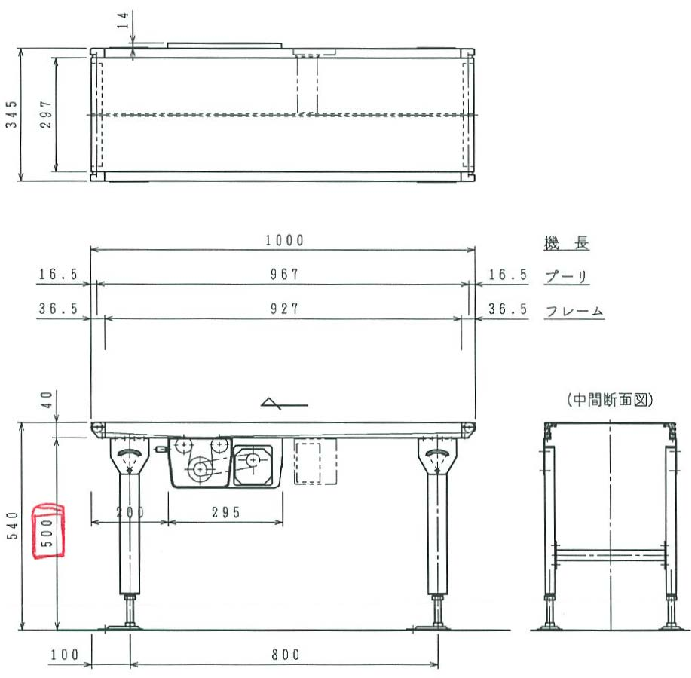
\includegraphics[width=.8\columnwidth, clip]{fig/4-manipulation-result/blueprint.pdf}
    \caption{The drawing of DMG(ベルコンミニ DMG 手配図より引用)}
    \label{The drawing of DMG}
\end{figure}

また,ハンドの関節には双葉電子工業株式会社製のサーボモータ RS405CBを使用した.
サーボモータの仕様を\tabref{table::servo}に,各装置の接続状況を\figref{fig::experimental-setup},\tabref{table::equipment}に示す.
このサーボモータには,指定した目標角度まで任意の時間で移動させるという機能がついている.実験ではこの機能を用いた.

以上のような実験環境のもと,\secref{sec::planner::intro}で設定した寸法と同様のロボットハンドと対象物を3Dプリンタにより作成し,マニピュレーション実験を行った.

\begin{figure}[b]
    \centering
    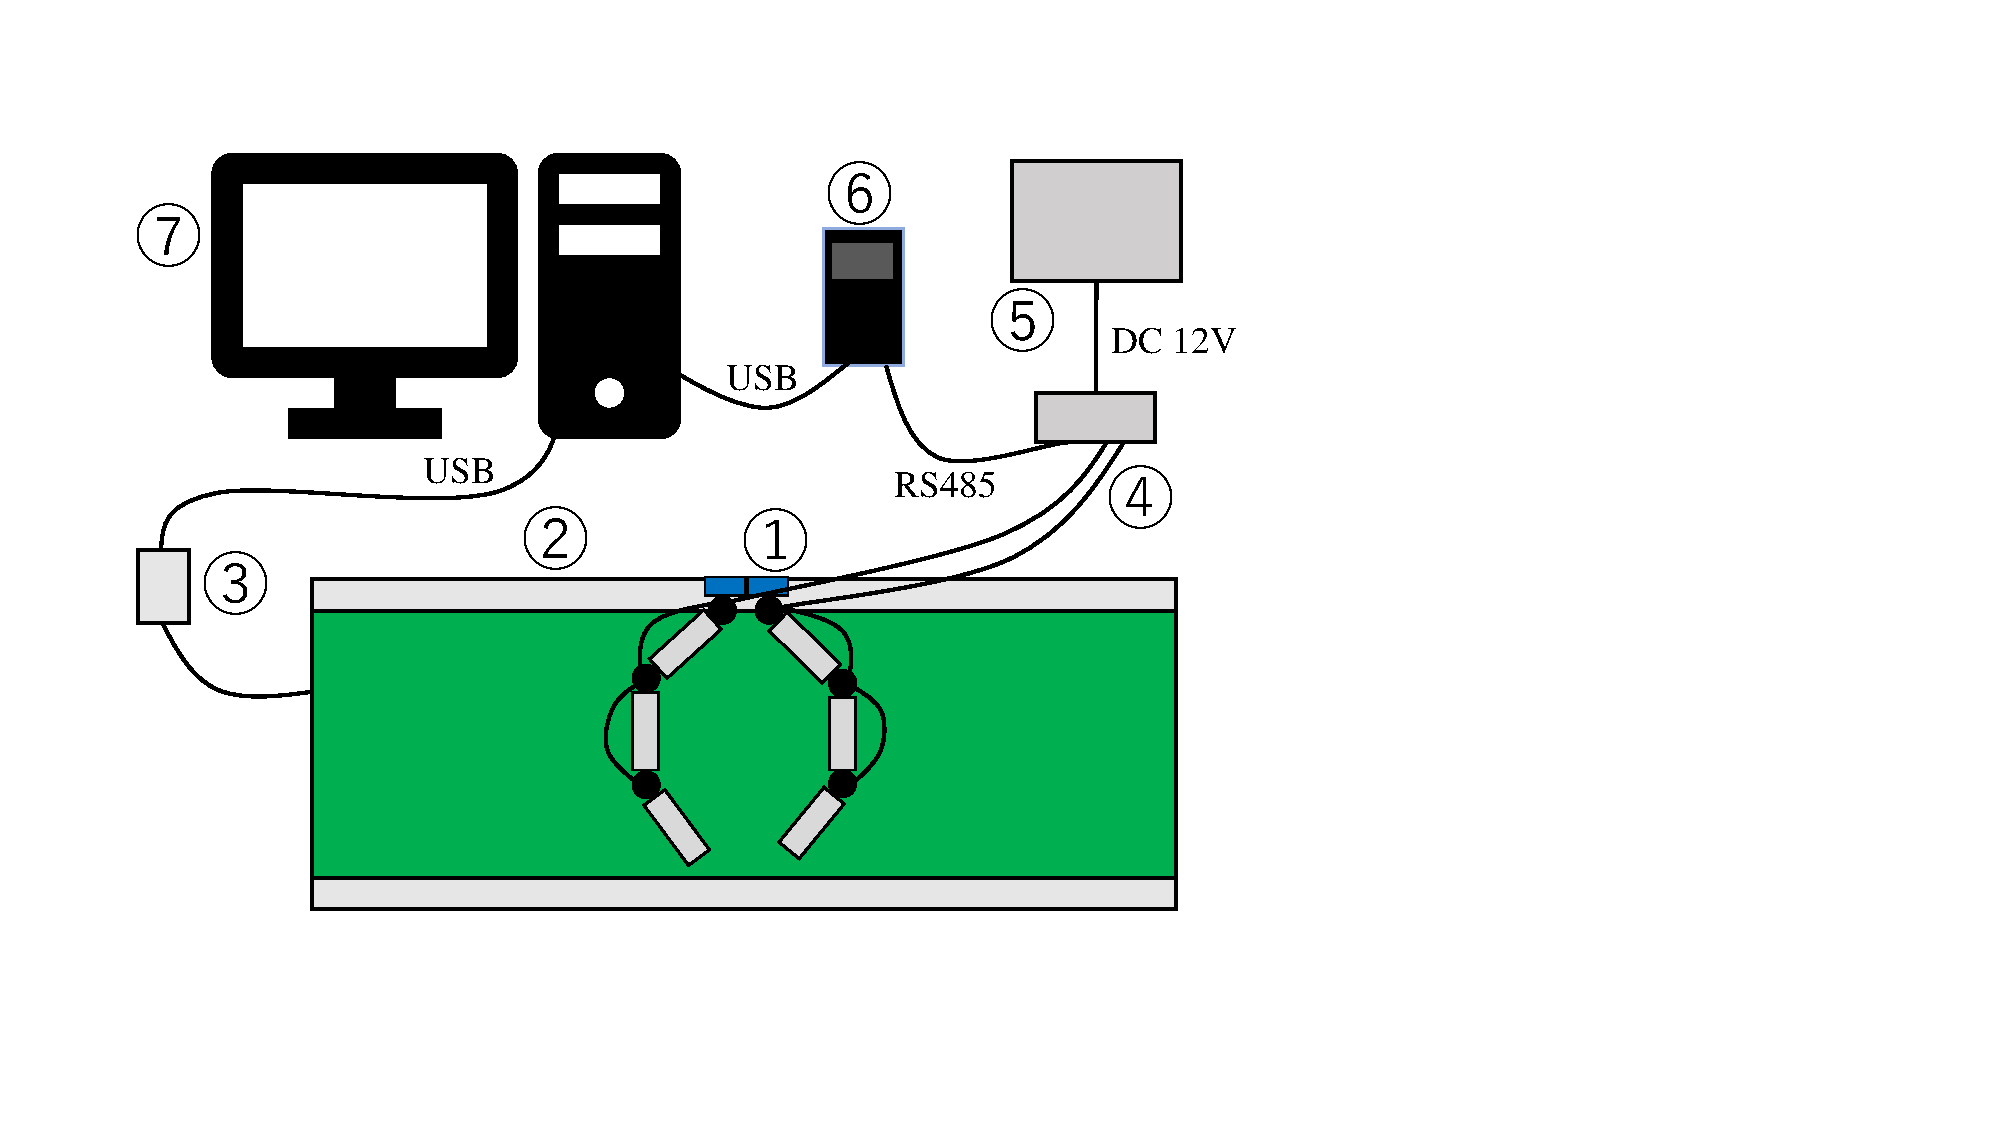
\includegraphics[width=1.\columnwidth, clip]{fig/4-manipulation-result/setup.pdf}
    \caption{The experimental setup \cite{kamikukita2022}}
    \label{fig::experimental-setup}
\end{figure}
\begin{table}[b]
    \centering
    \caption{Specifications of the servomotor}
    \begin{tabular}{|c|c|}
    \hline
    寸法 & $40.5 \times 21.0 \times 41.8$ [mm] \\
    \hline
    質量 & 67 [g] \\
    \hline
    出力トルク & 48.0 [$\mathrm{kg} \cdot \mathrm{cm}$] (11.1 V時) \\
    \hline
    動作スピード & 0.21 [sec/60度] (11.1 V時) \\
    \hline
    \multirow{2}{*}{動作角度} & 150 [度] (コマンド方式) / 144 [度] (PWM方式) \\
            & 150 [度] (コマンド方式) / 144 [度] (PWM方式) \\
    \hline
    \multirow{2}{*}{特徴} & RS485非同期通信コマンド方式 \\
        & ブラシレスモータ採用 \\
    \hline
    \end{tabular}
    \label{table::servo}
\end{table}
\begin{table}[b]
    \centering
    \caption{Equipment \cite{kamikukita2022}}
    \begin{tabular}{|c|c|}
    \hline
    1. アクチュエータ & RS405CB (双葉電子工業) \\
    \hline
    2. ベルトコンベア & ベルコンミニI\hspace{-.1em}I\hspace{-.1em}I DMG (オークラ輸送機) \\
    \hline
    3. リレーモジュール & URMC2 2ch USBリレー (Numato Lab) \\
    \hline
    4. ハブ & TB-RV71EH-7.4V/4W (双葉電子工業) \\
    \hline
    5. スイッチング電源 & ESP10-15-12 (MISUMI) \\
    \hline
    6. シリアル変換器 & CONVERTER RSC-U485 JPN (双葉電子工業) \\
    \hline
    \multirow{2}{*}{7. 制御用PC} & OS:Windows10 \\
        & CPU:Ryzen 7 3700X / 3.6GHz \\
    \hline
    \end{tabular}
    \label{table::equipment}
\end{table}
%ベルトコンベアとか3Dプリンタで作ったとかサーボモータとか

\section{長方形のマニピュレーション}
本節では,長方形物体を対象としたマニピュレーション結果を示す.タスクは,ベルトコンベアに乗って流れてきた対象物を,ベルト幅中央に$90^\circ$で整列させる,というように設定した.動作計画には,順探索アルゴリズムを用いた.入力情報を以下にまとめる.
\begin{gather}
\notag
\left\{
\begin{aligned}
&ハンド初期姿勢:[\theta_1, \theta_2, \theta_3, \theta_4, \theta_5, \theta_6,] = [25, -30, -75, 30, -30, -20]\mathrm{[deg]}\\
&対象物の目標位置・姿勢:[x_{\mathrm {goal}}, y_{\mathrm {goal}}, \phi_{\mathrm {goal}}] = [{\mathrm {any}}, 200 \mathrm{[mm]}, 90 \mathrm{[deg]}]\\
&順探索の終了閾値:\varepsilon = 50\\
\end{aligned}
\right .
\end{gather}
動作計画にかかった計算時間は[s]であり,
この経路を用いて長方形物体の異なる2つの初期位置・姿勢に対してマニピュレーションを行った.
結果を\figref{fig::result::rm1},\figref{fig::result::rm2}に示す.
\begin{figure}[hbt]
\centering
\begin{minipage}{0.249\hsize}
\centering
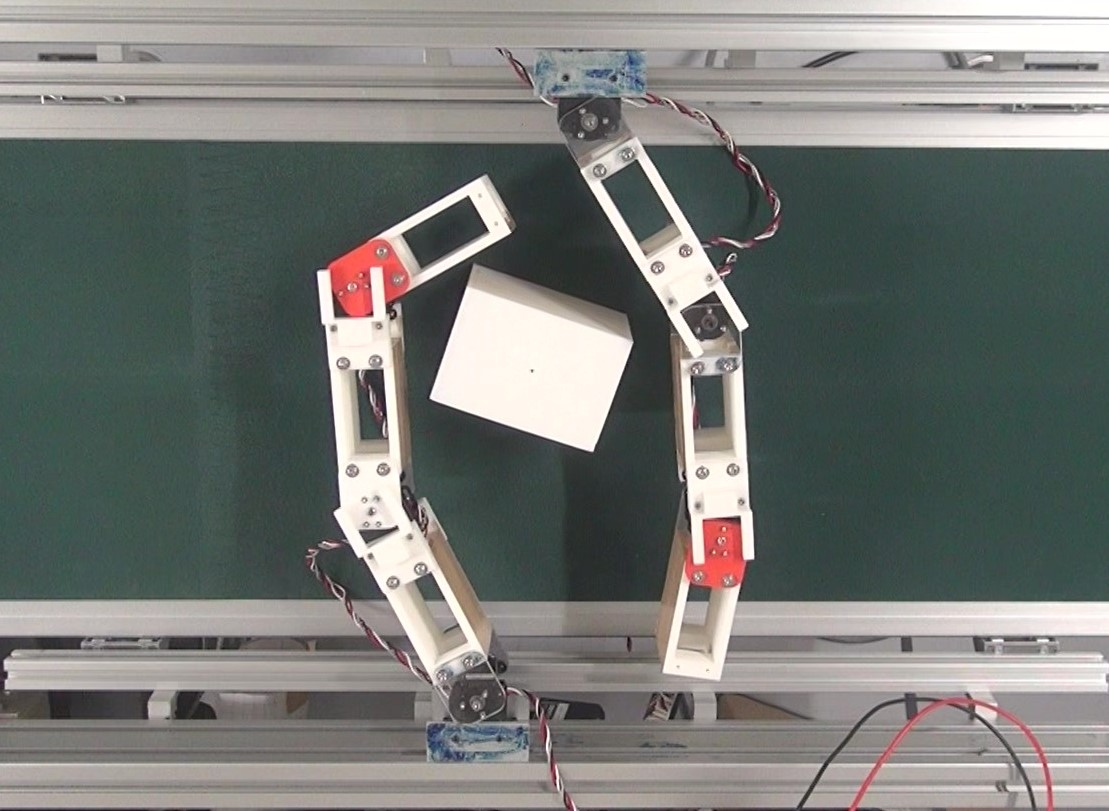
\includegraphics[width=0.98\hsize]{fig/4-manipulation-result/Rectangle/1-1.jpg}
\subcaption{}\label{}
\end{minipage}\hfill
\begin{minipage}{0.249\hsize}
\centering
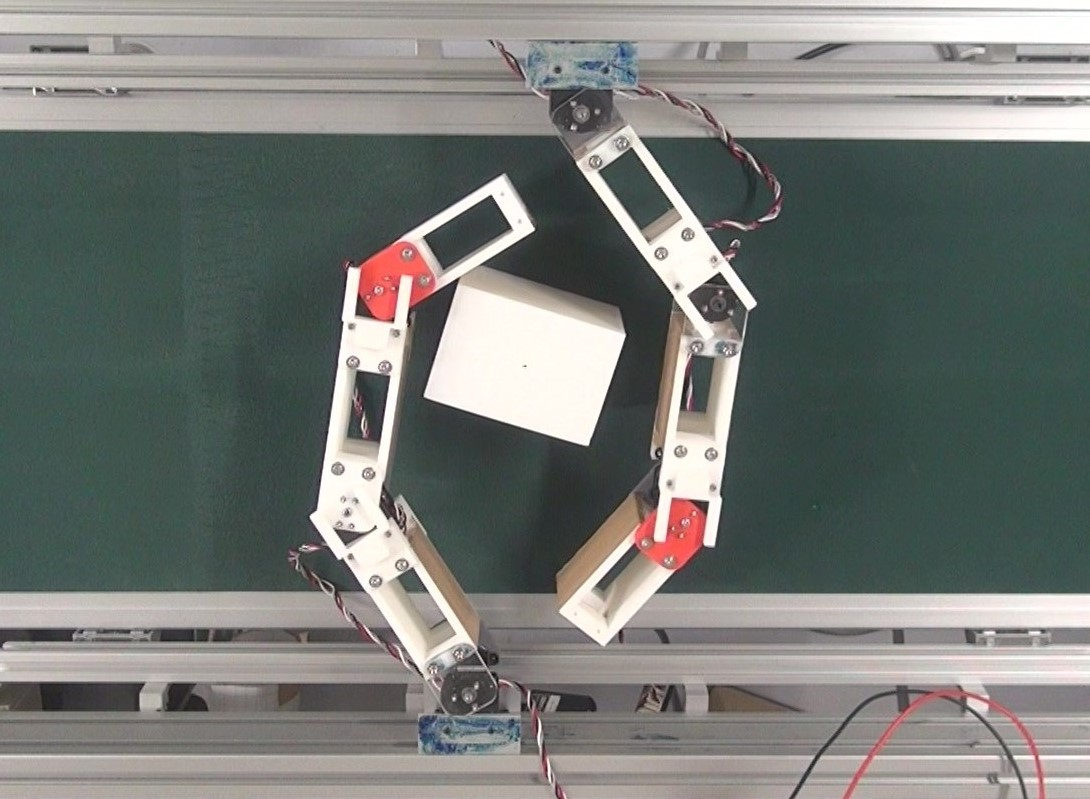
\includegraphics[width=0.98\hsize]{fig/4-manipulation-result/Rectangle/1-2.jpg}
\subcaption{}\label{}
\end{minipage}\hfill
\begin{minipage}{0.249\hsize}
\centering
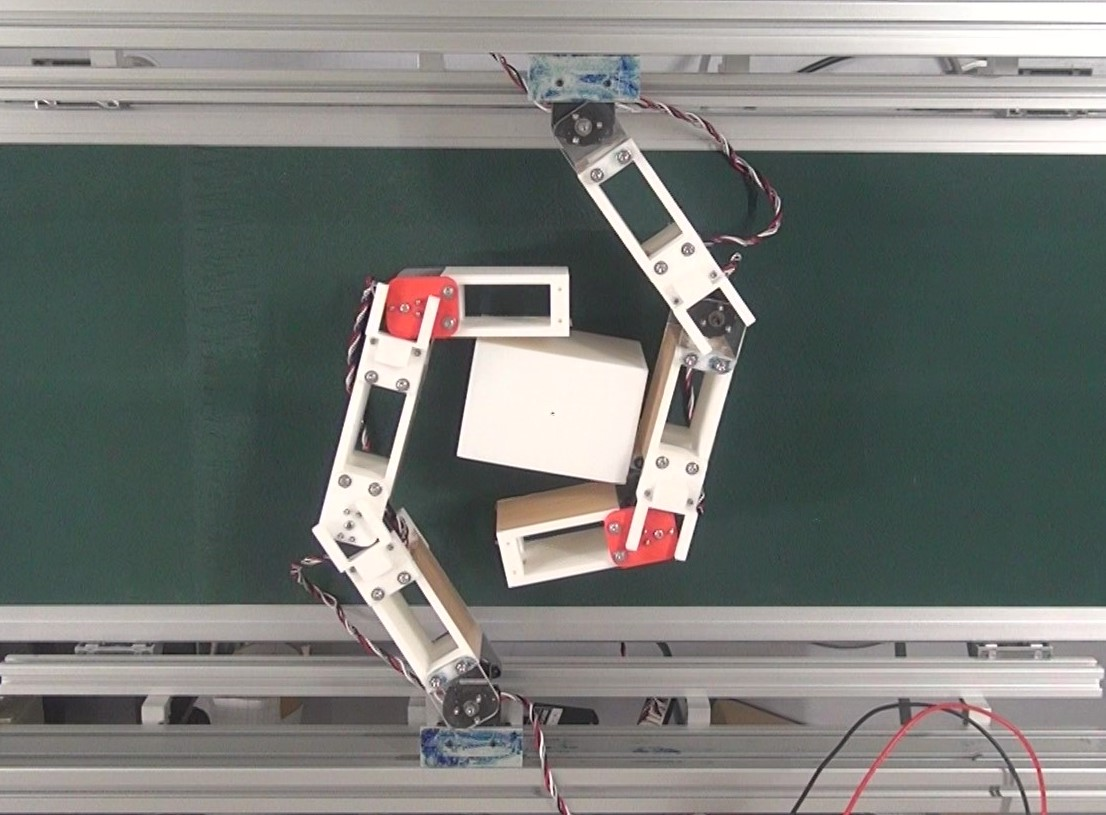
\includegraphics[width=0.98\hsize]{fig/4-manipulation-result/Rectangle/1-3.jpg}
\subcaption{}\label{}
\end{minipage}\hfill
\begin{minipage}{0.249\hsize}
\centering
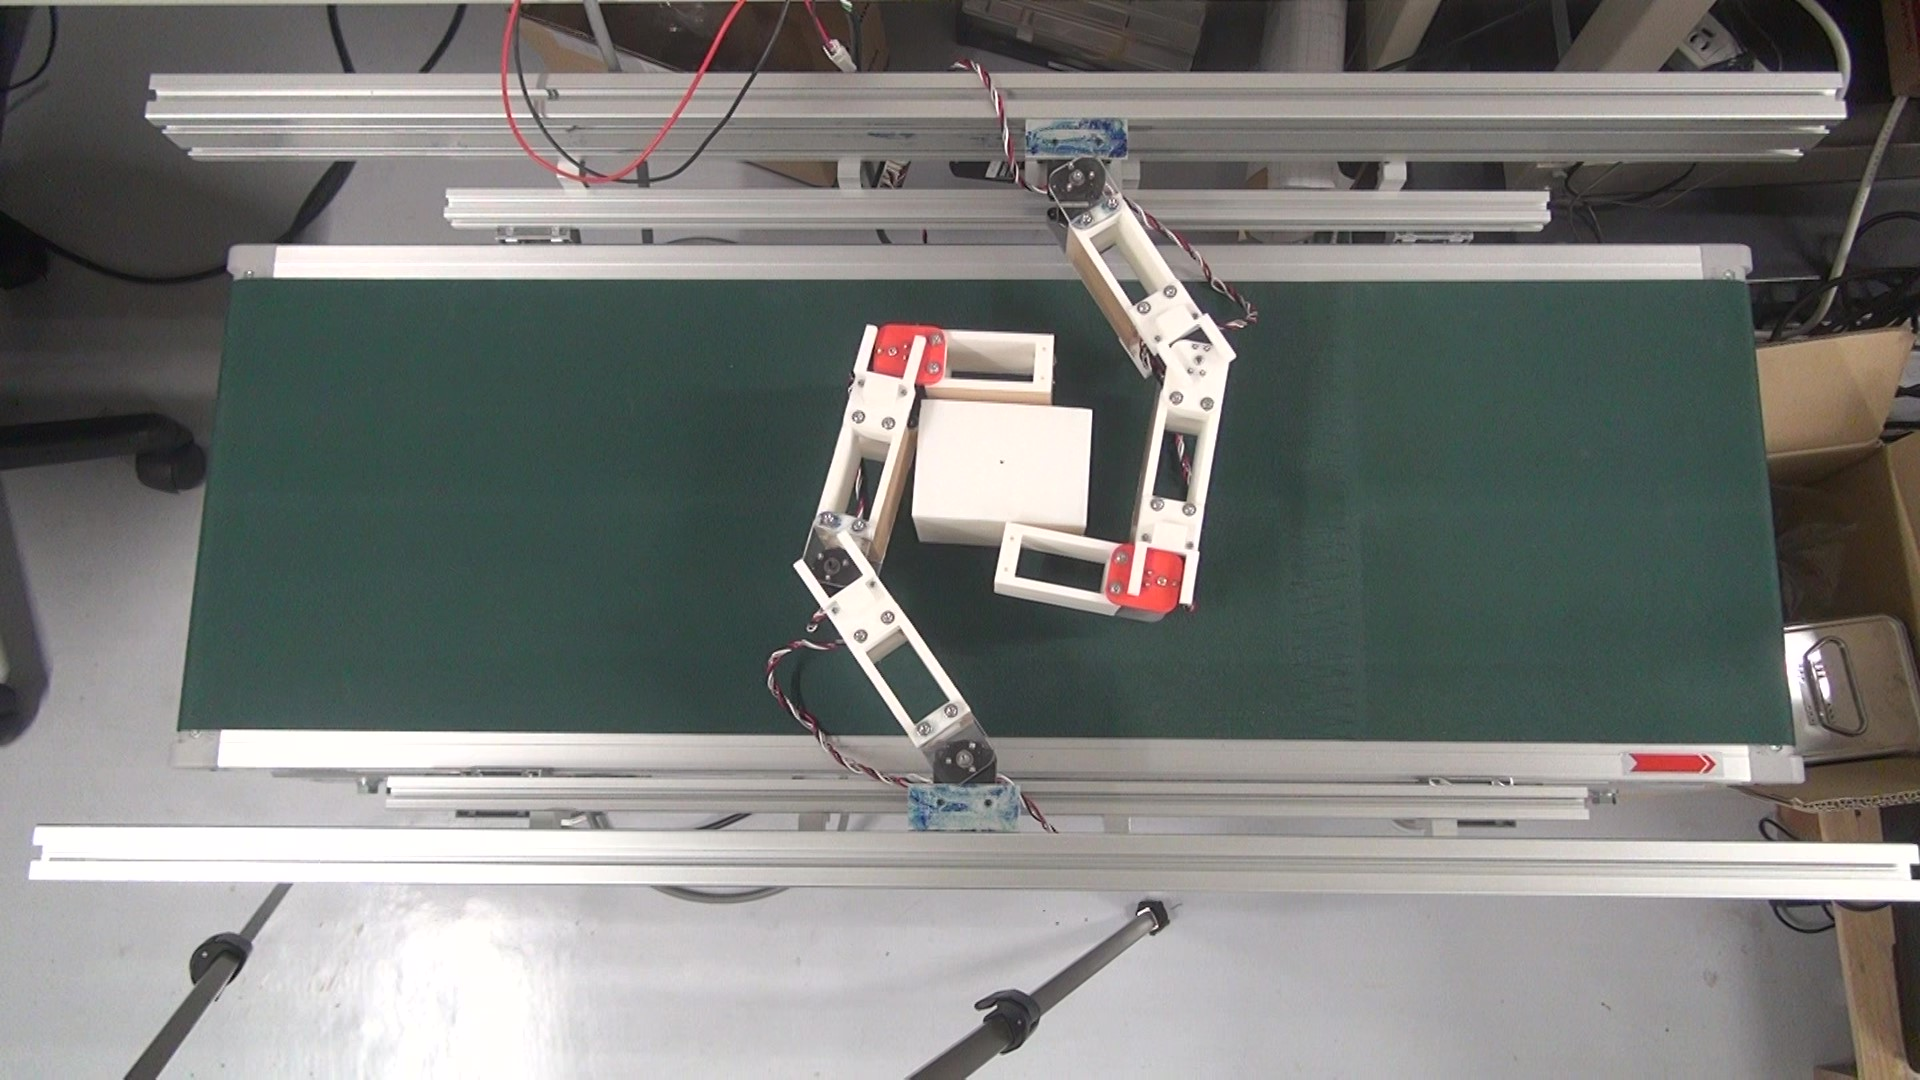
\includegraphics[width=0.98\hsize]{fig/4-manipulation-result/Rectangle/1-4.jpg}
\subcaption{}\label{}
\end{minipage}
\caption{Rectangle manipulation result \#1}\label{fig::result::rm1}
\end{figure}

\begin{figure}[hbt]
\centering
\begin{minipage}{0.249\hsize}
\centering
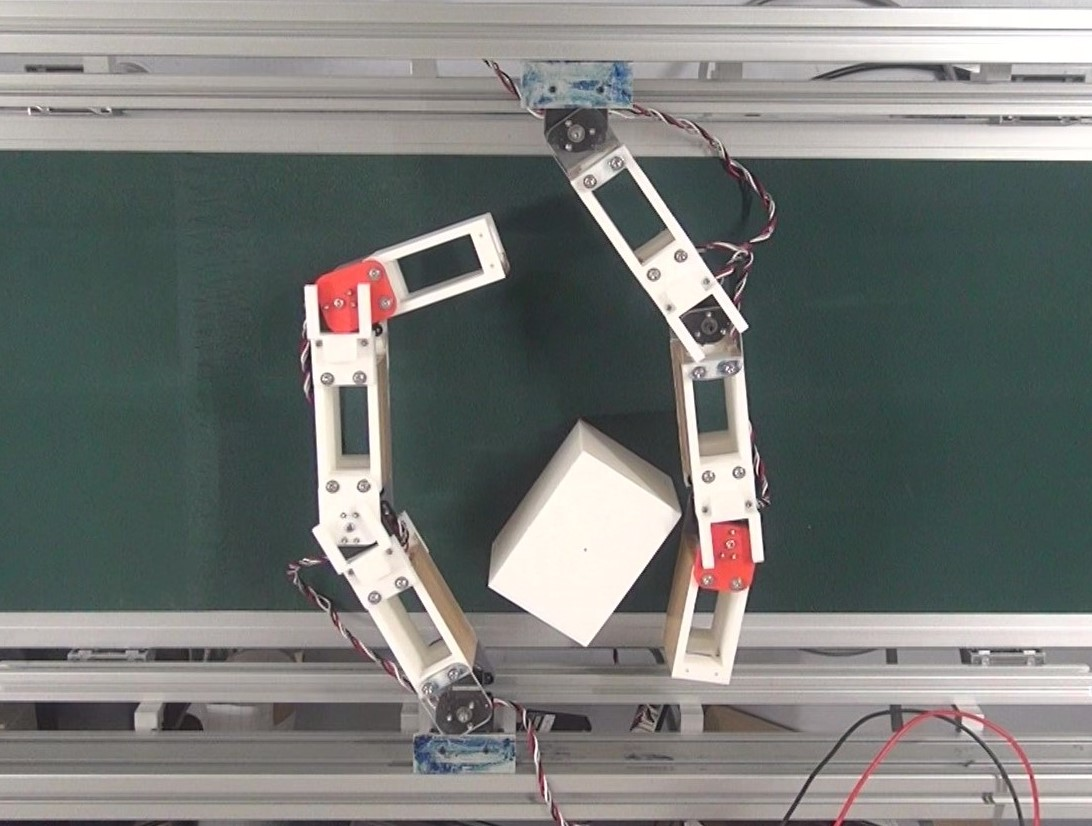
\includegraphics[width=0.98\hsize]{fig/4-manipulation-result/Rectangle/2-1.jpg}
\subcaption{}\label{}
\end{minipage}\hfill
\begin{minipage}{0.249\hsize}
\centering
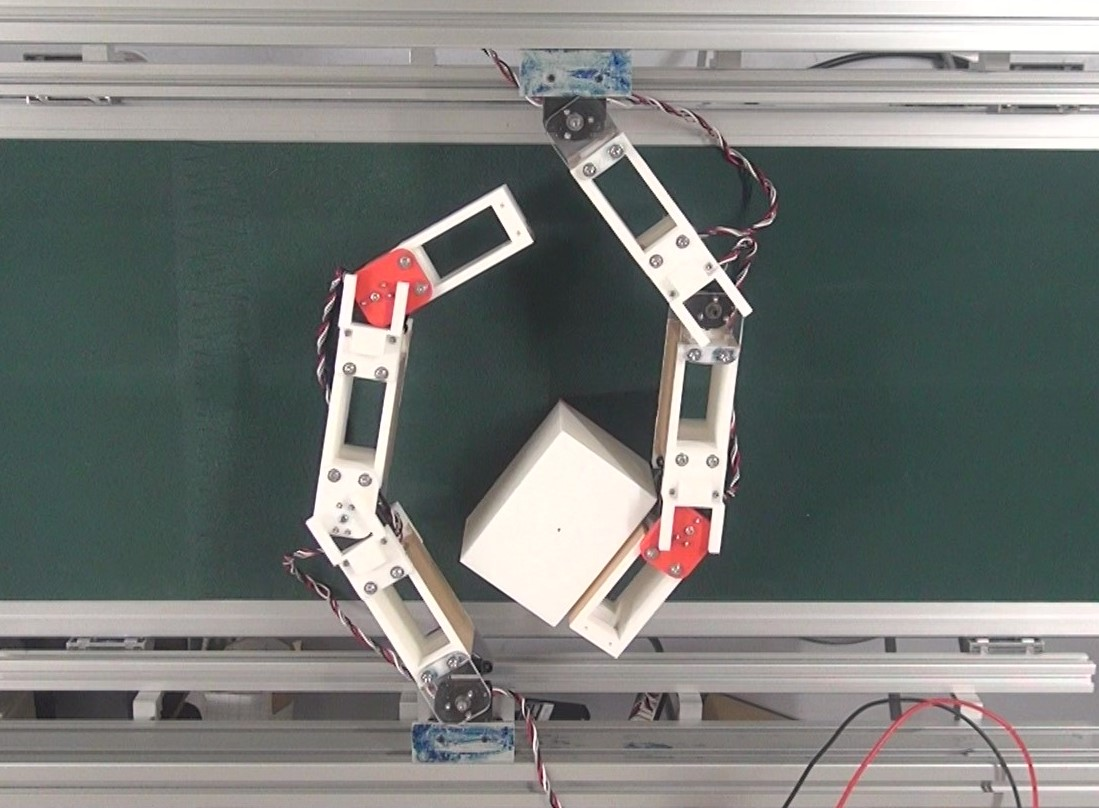
\includegraphics[width=0.98\hsize]{fig/4-manipulation-result/Rectangle/2-2.jpg}
\subcaption{}\label{}
\end{minipage}\hfill
\begin{minipage}{0.249\hsize}
\centering
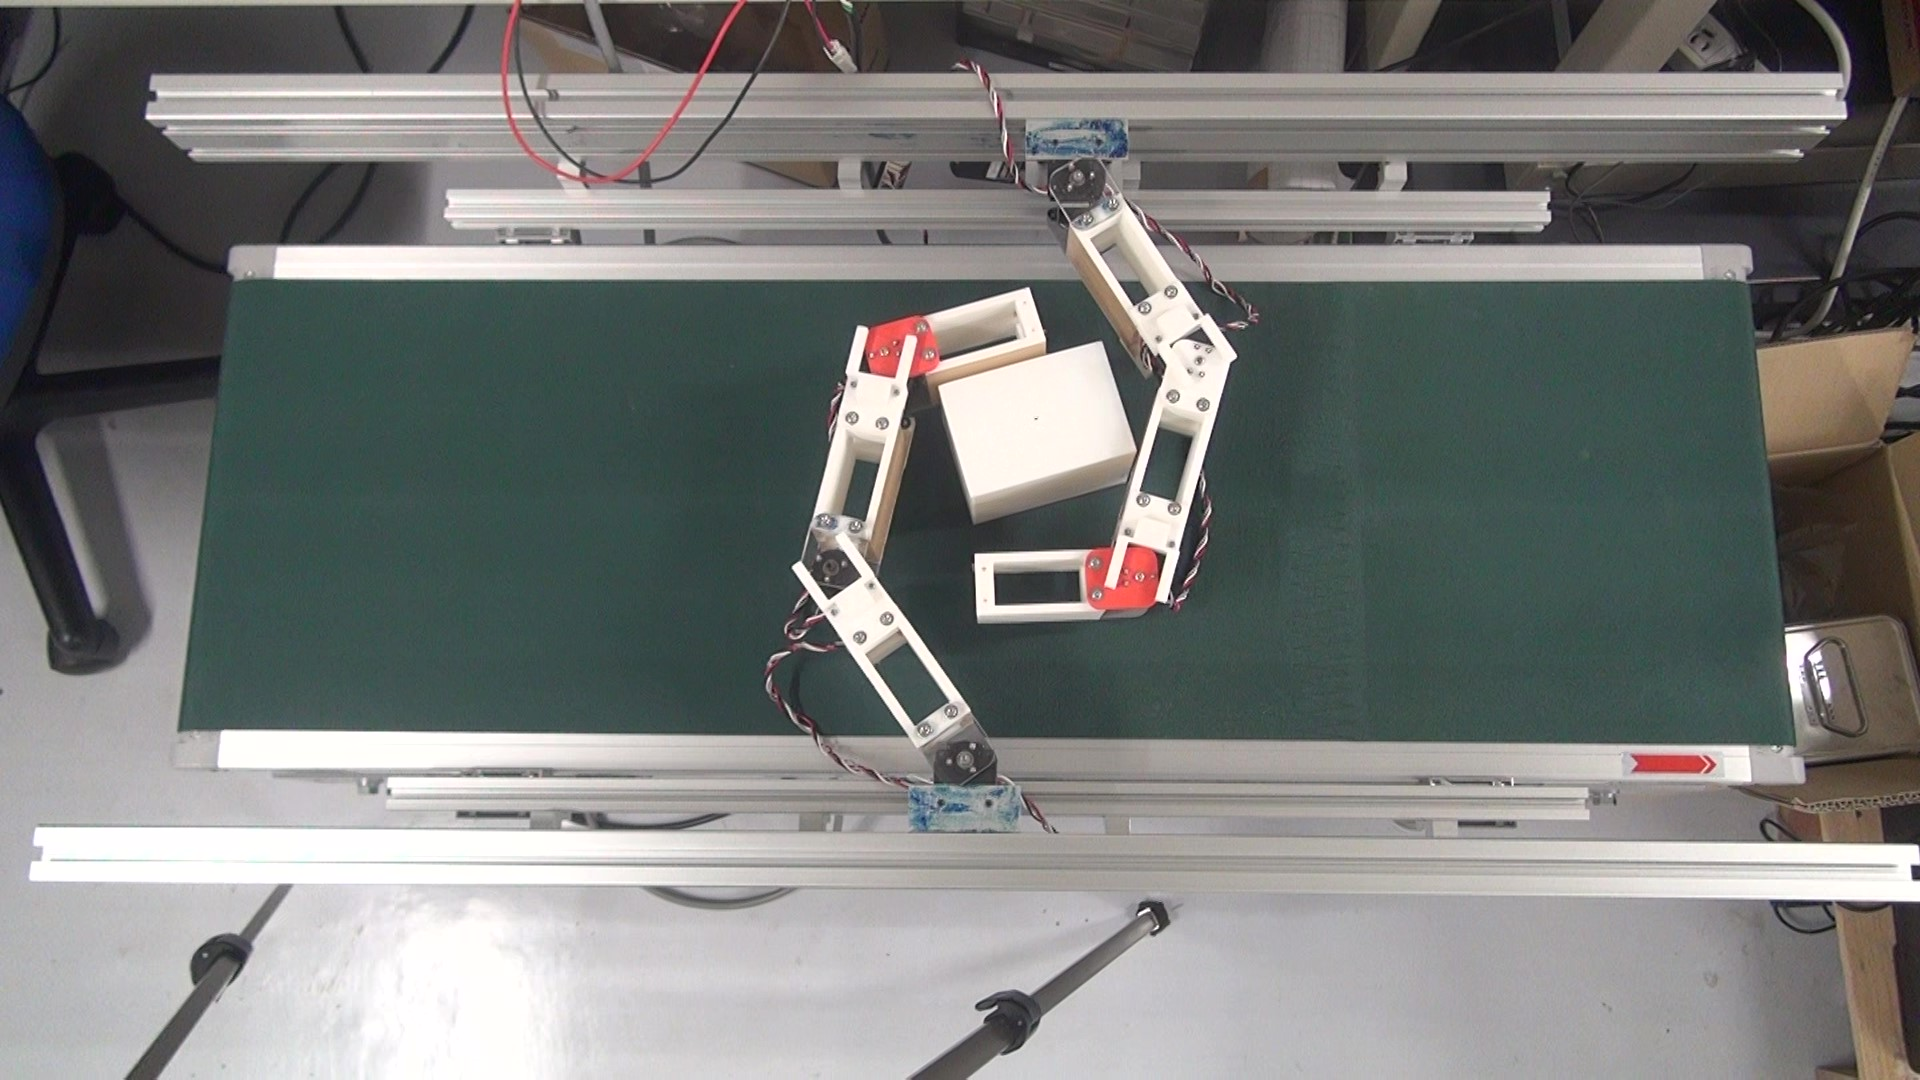
\includegraphics[width=0.98\hsize]{fig/4-manipulation-result/Rectangle/2-3.jpg}
\subcaption{}\label{}
\end{minipage}\hfill
\begin{minipage}{0.249\hsize}
\centering
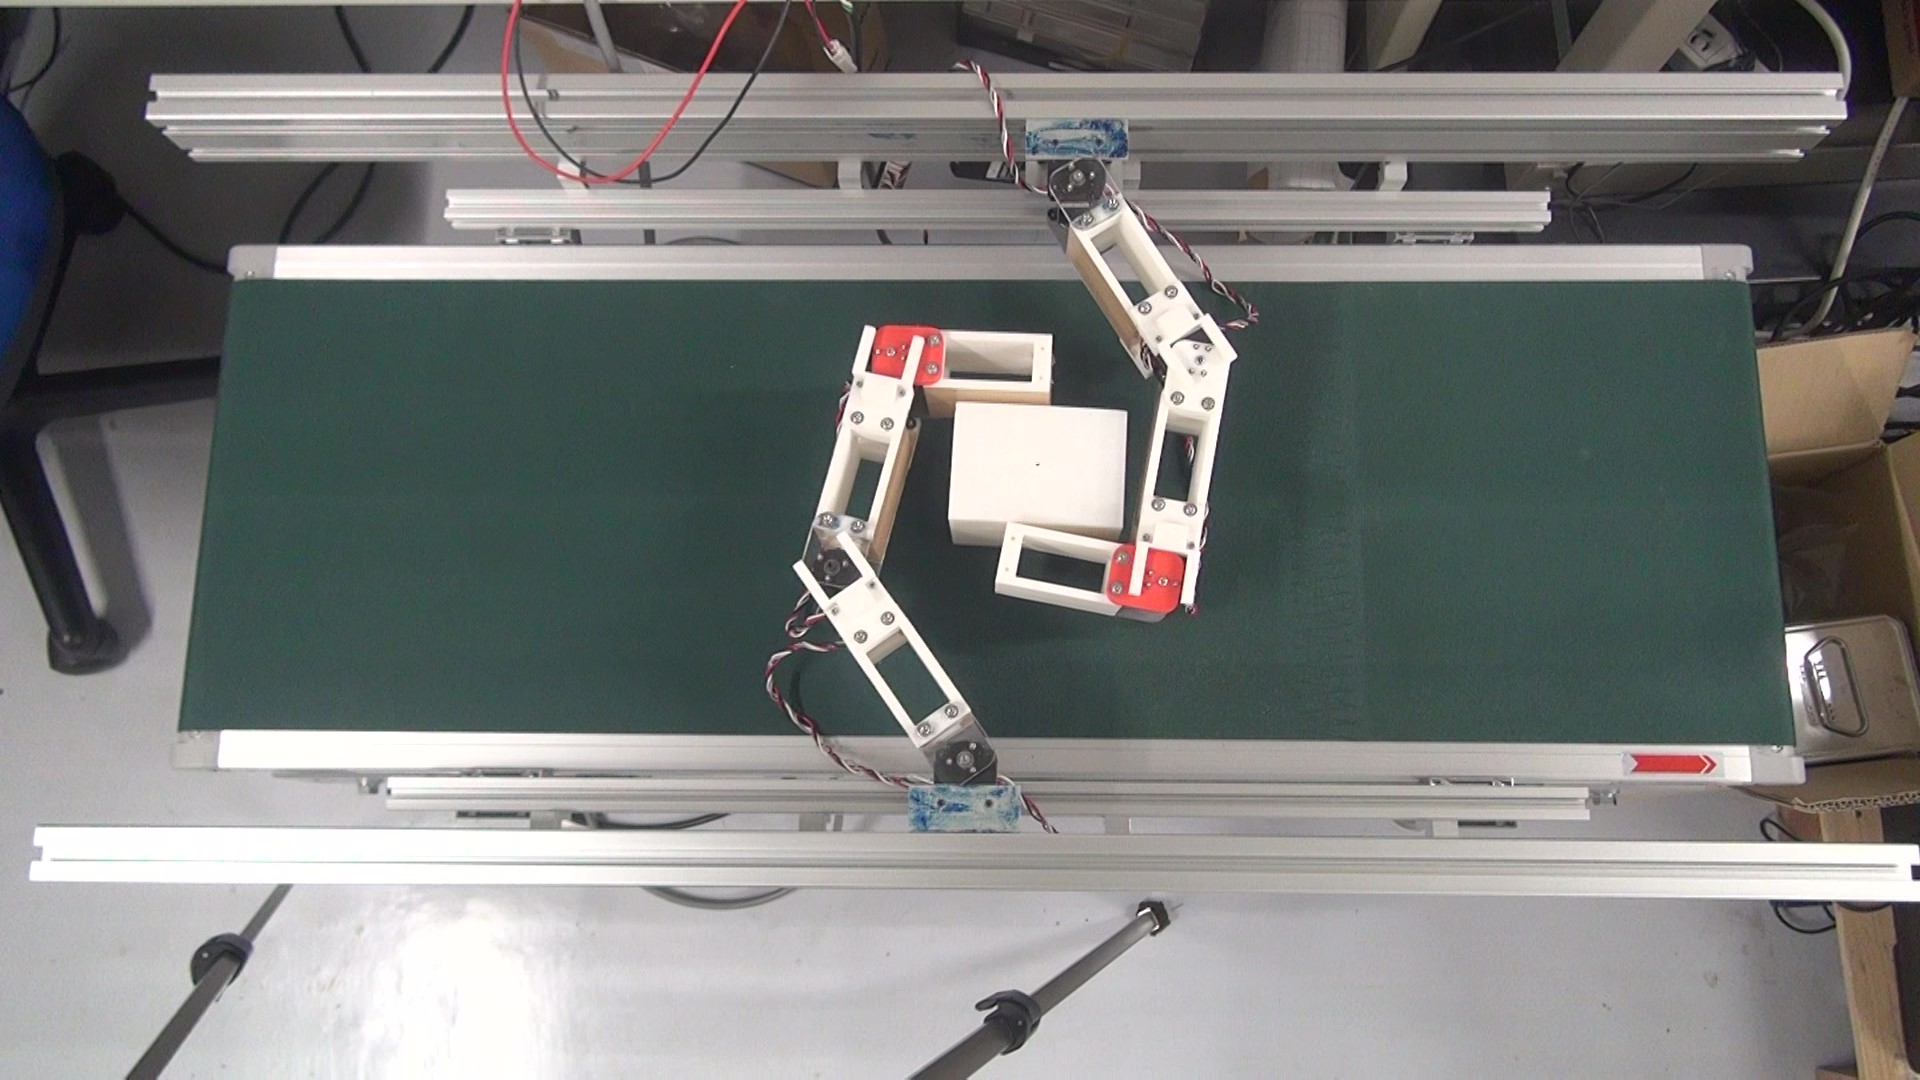
\includegraphics[width=0.98\hsize]{fig/4-manipulation-result/Rectangle/2-4.jpg}
\subcaption{}\label{}
\end{minipage}
\caption{Rectangle manipulation result \#2}\label{fig::result::rm2}
\end{figure}

\figref{fig::result::rm1}のマニピュレーション後の対象物位置・姿勢は,$(x, y, \phi) = (10 \mathrm{[mm]}, 204 \mathrm{[mm]}, 87 \mathrm{[deg]})$であり,目標位置・姿勢から$\Delta y = +4 \mathrm{[mm]}$,$\Delta \phi = -3 \mathrm{[deg]}$の誤差があった.また,\figref{fig::result::rm2}のマニピュレーション後の対象物位置・姿勢は,$(x, y, \phi) = (-3 \mathrm{[mm]}, 202 \mathrm{[mm]}, 88 \mathrm{[deg]})$であり,目標位置・姿勢から$\Delta y = +2 \mathrm{[mm]}$,$\Delta \phi = -2 \mathrm{[deg]}$の誤差があった.\par

次に,パーツフィーダとしての動作結果を\figref{fig::result::rp}に示す.これより,L字形物体に対してキャッチ,整列,リリースの一連のタスクを行えることを確認した.
\begin{figure}[hb]
\centering
\begin{minipage}{0.49\hsize}
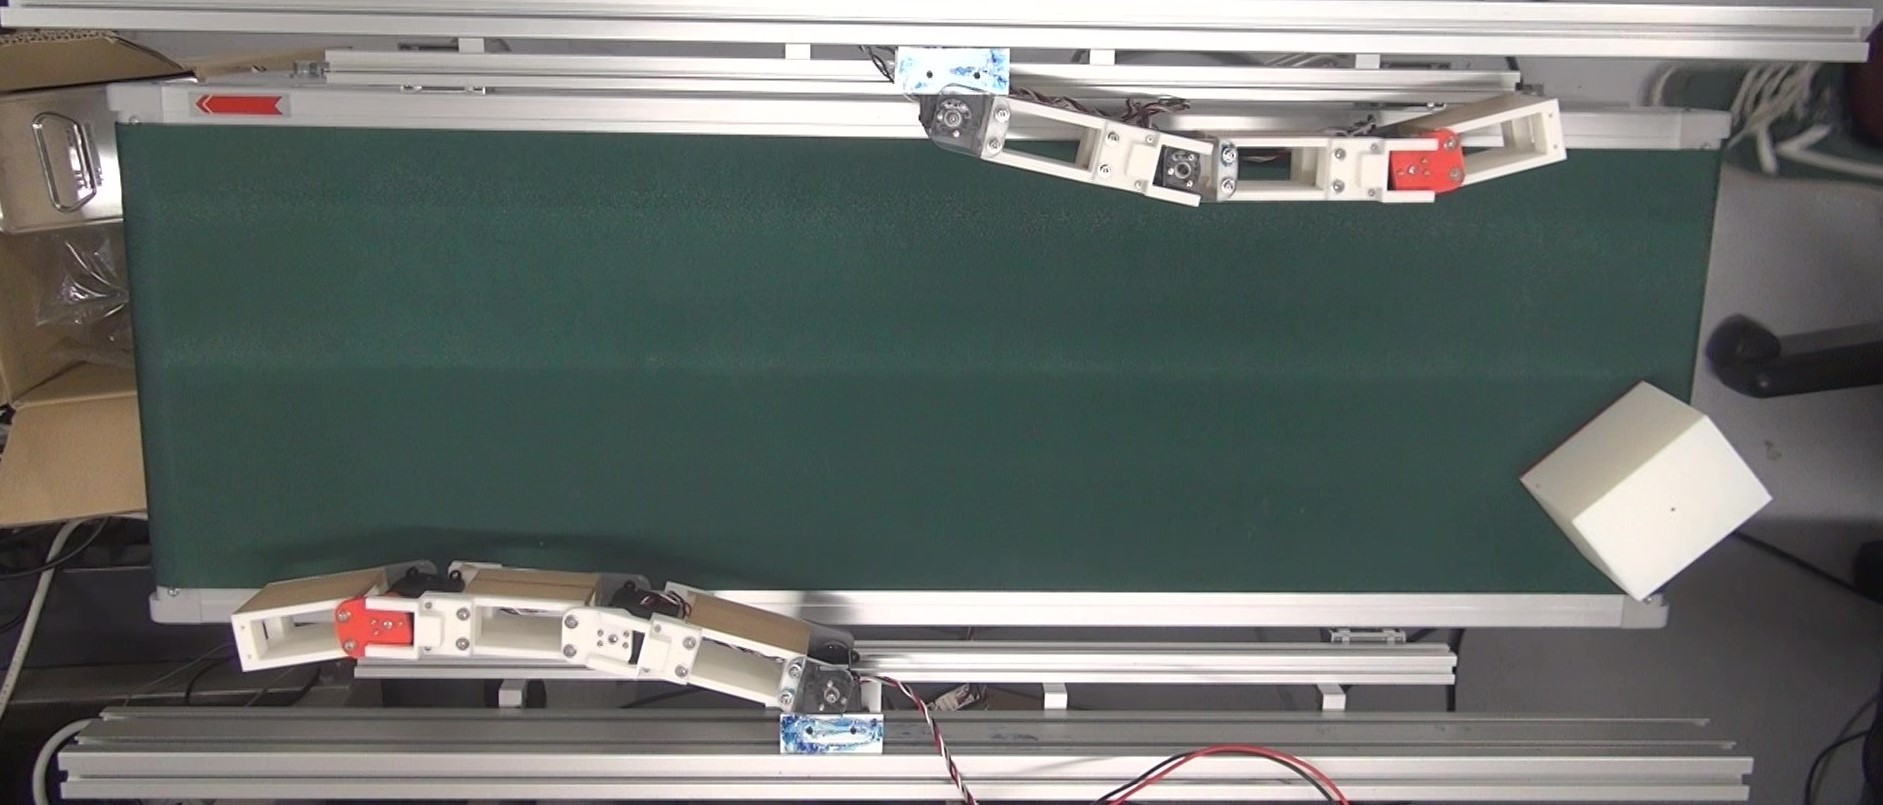
\includegraphics[width=0.98\hsize]{fig/4-manipulation-result/Rectangle/3-1.jpg}
\subcaption{}
\end{minipage}\hfill
\begin{minipage}{0.49\hsize}
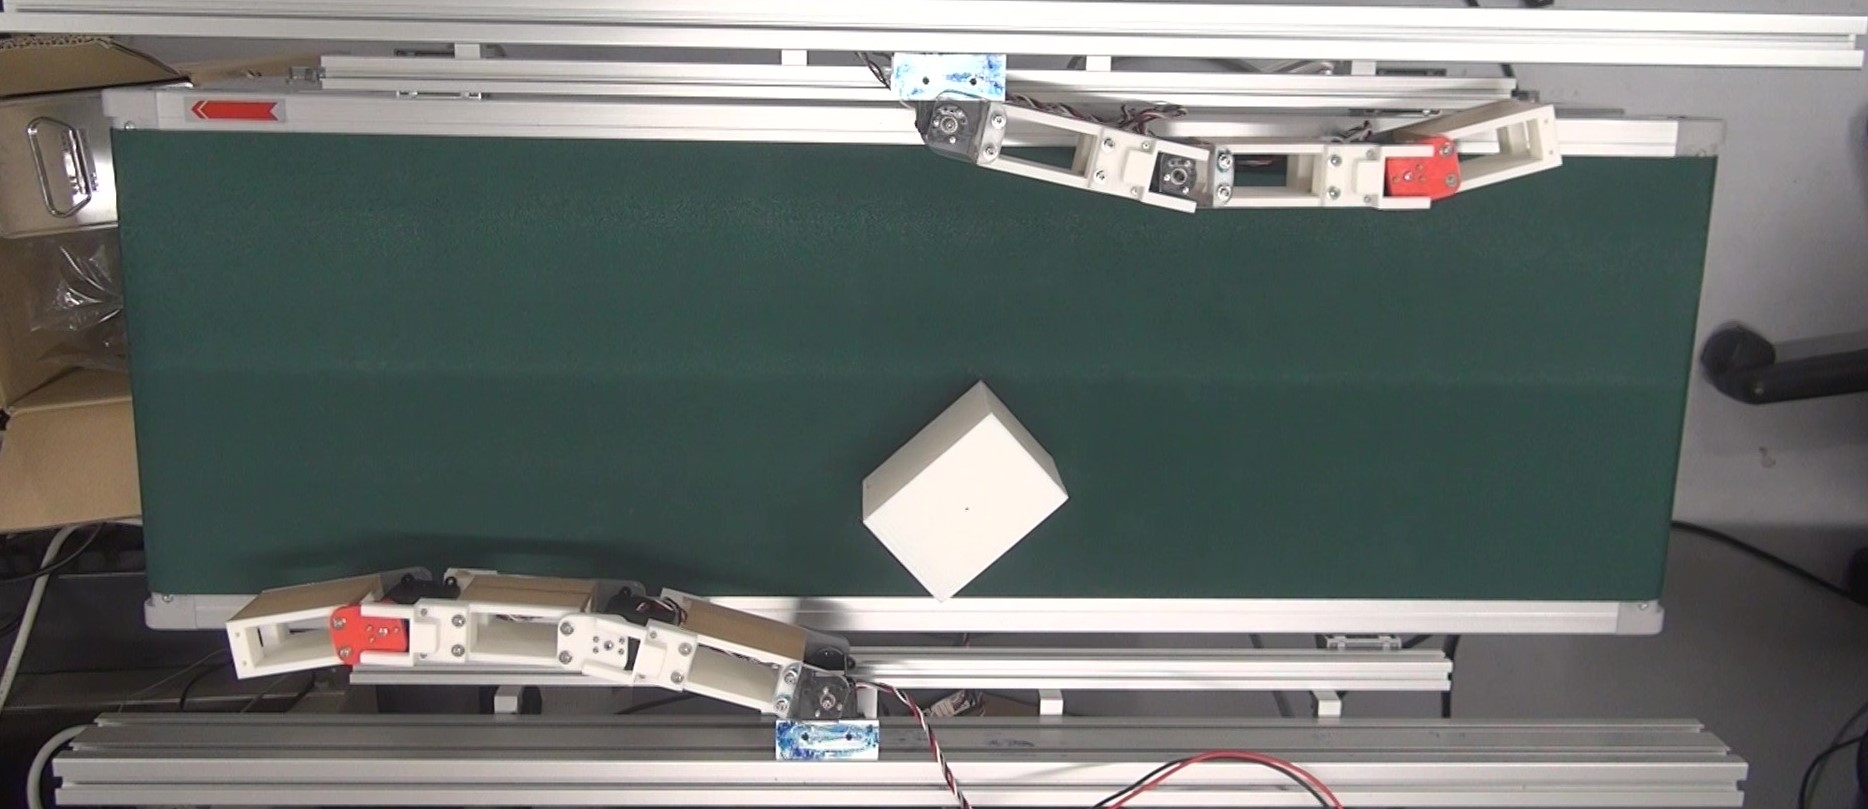
\includegraphics[width=0.98\hsize]{fig/4-manipulation-result/Rectangle/3-2.jpg}
\subcaption{}
\end{minipage}\hfill
\begin{minipage}{0.49\hsize}
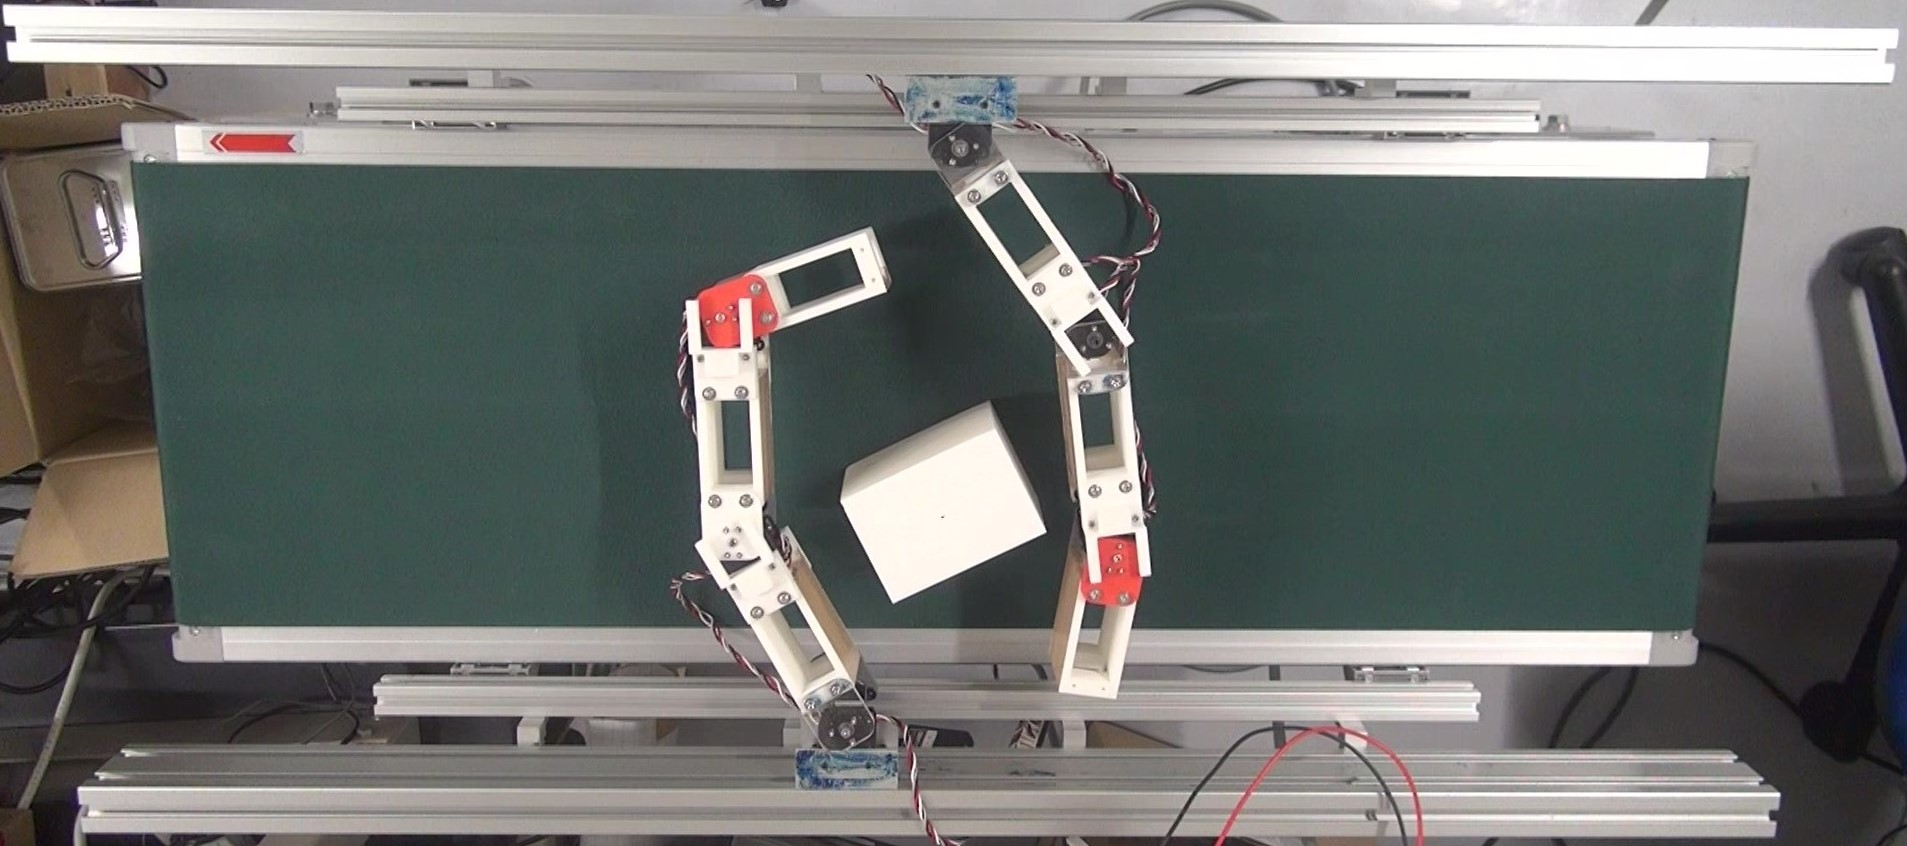
\includegraphics[width=0.98\hsize]{fig/4-manipulation-result/Rectangle/3-3.jpg}
\subcaption{}
\end{minipage}\hfill
\begin{minipage}{0.49\hsize}
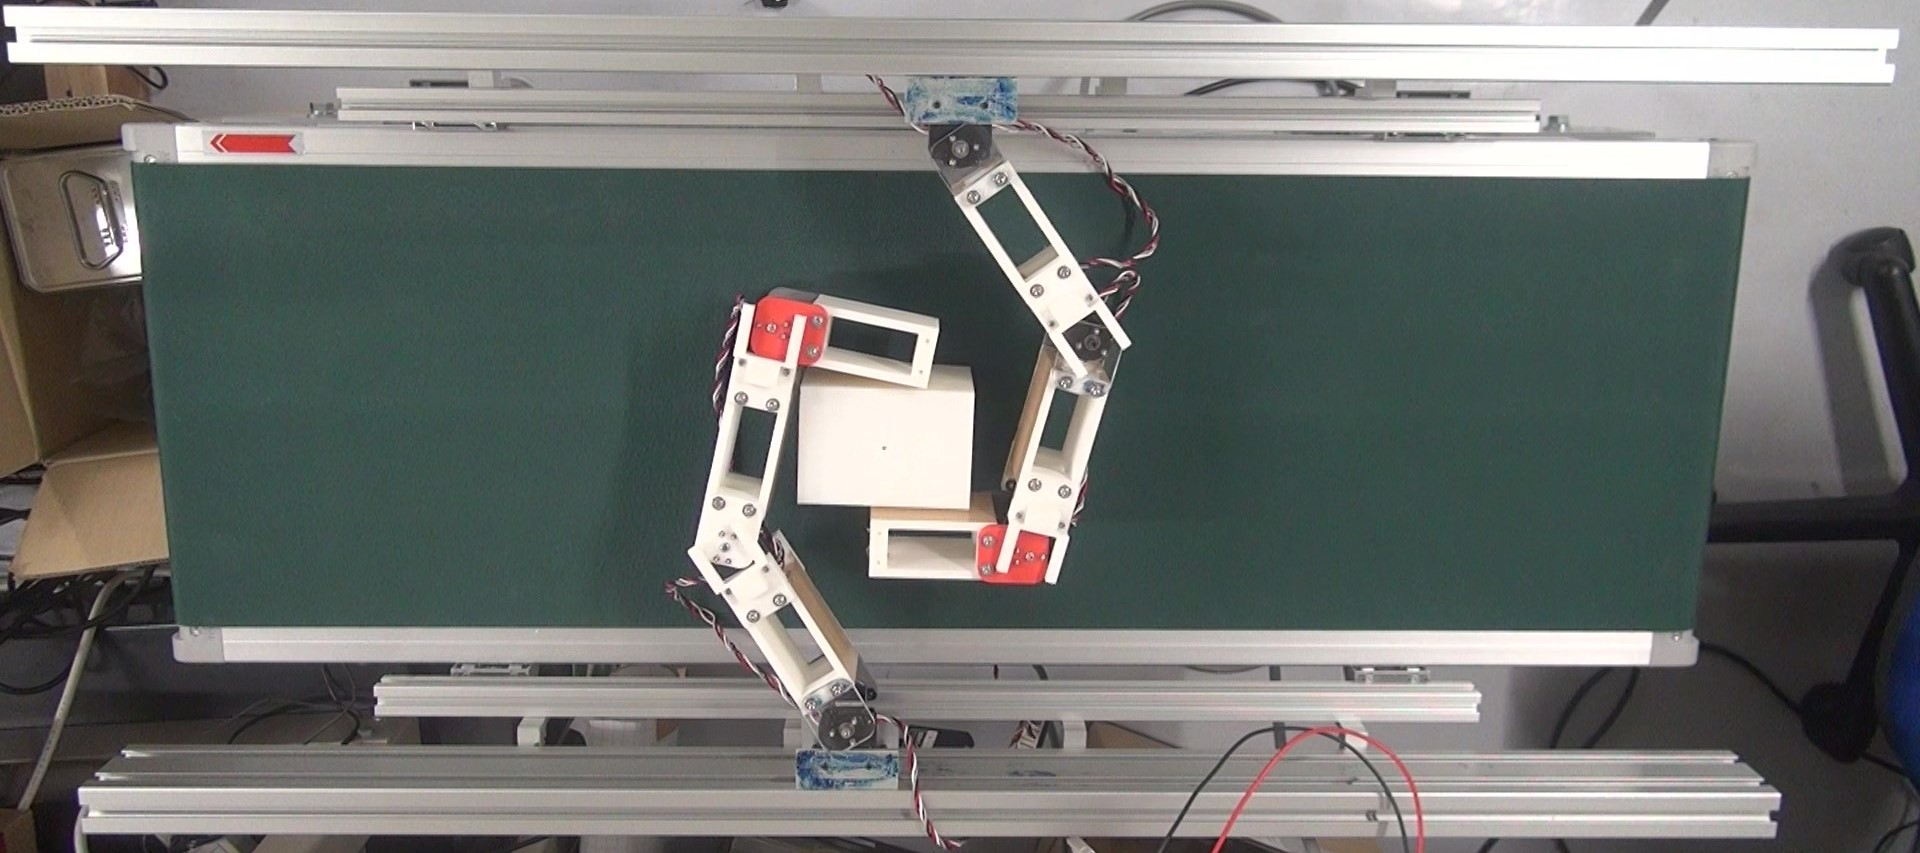
\includegraphics[width=0.98\hsize]{fig/4-manipulation-result/Rectangle/3-4.jpg}
\subcaption{}
\end{minipage}\hfill
\begin{minipage}{0.49\hsize}
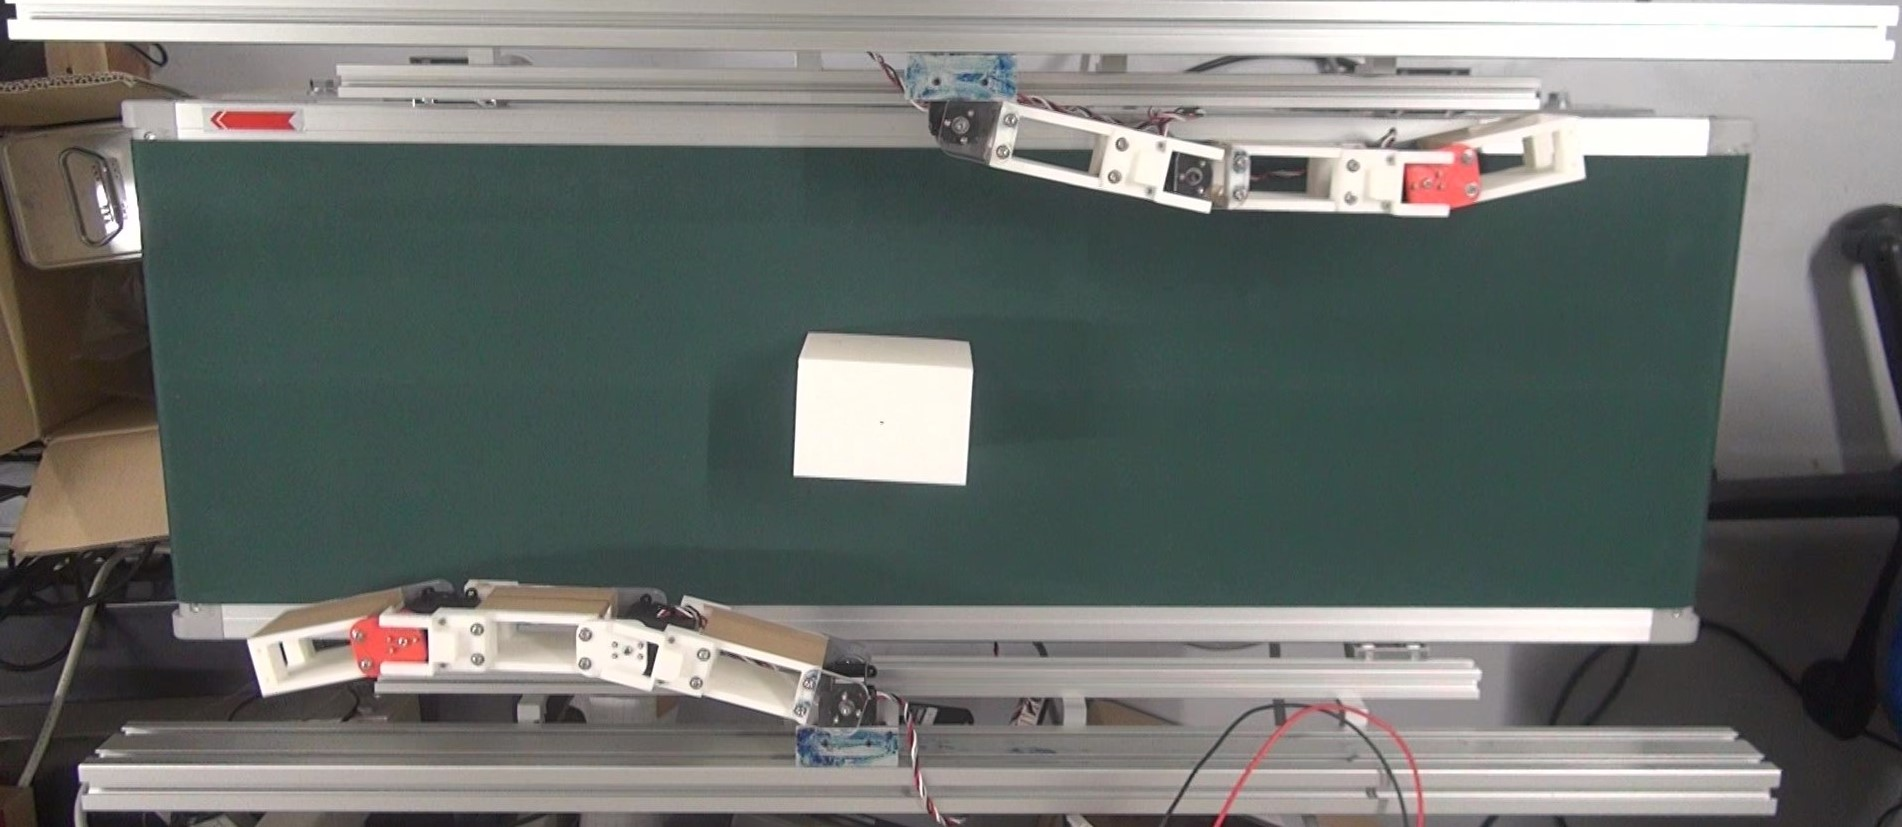
\includegraphics[width=0.98\hsize]{fig/4-manipulation-result/Rectangle/3-5.jpg}
\subcaption{}
\end{minipage}\hfill
\begin{minipage}{0.49\hsize}
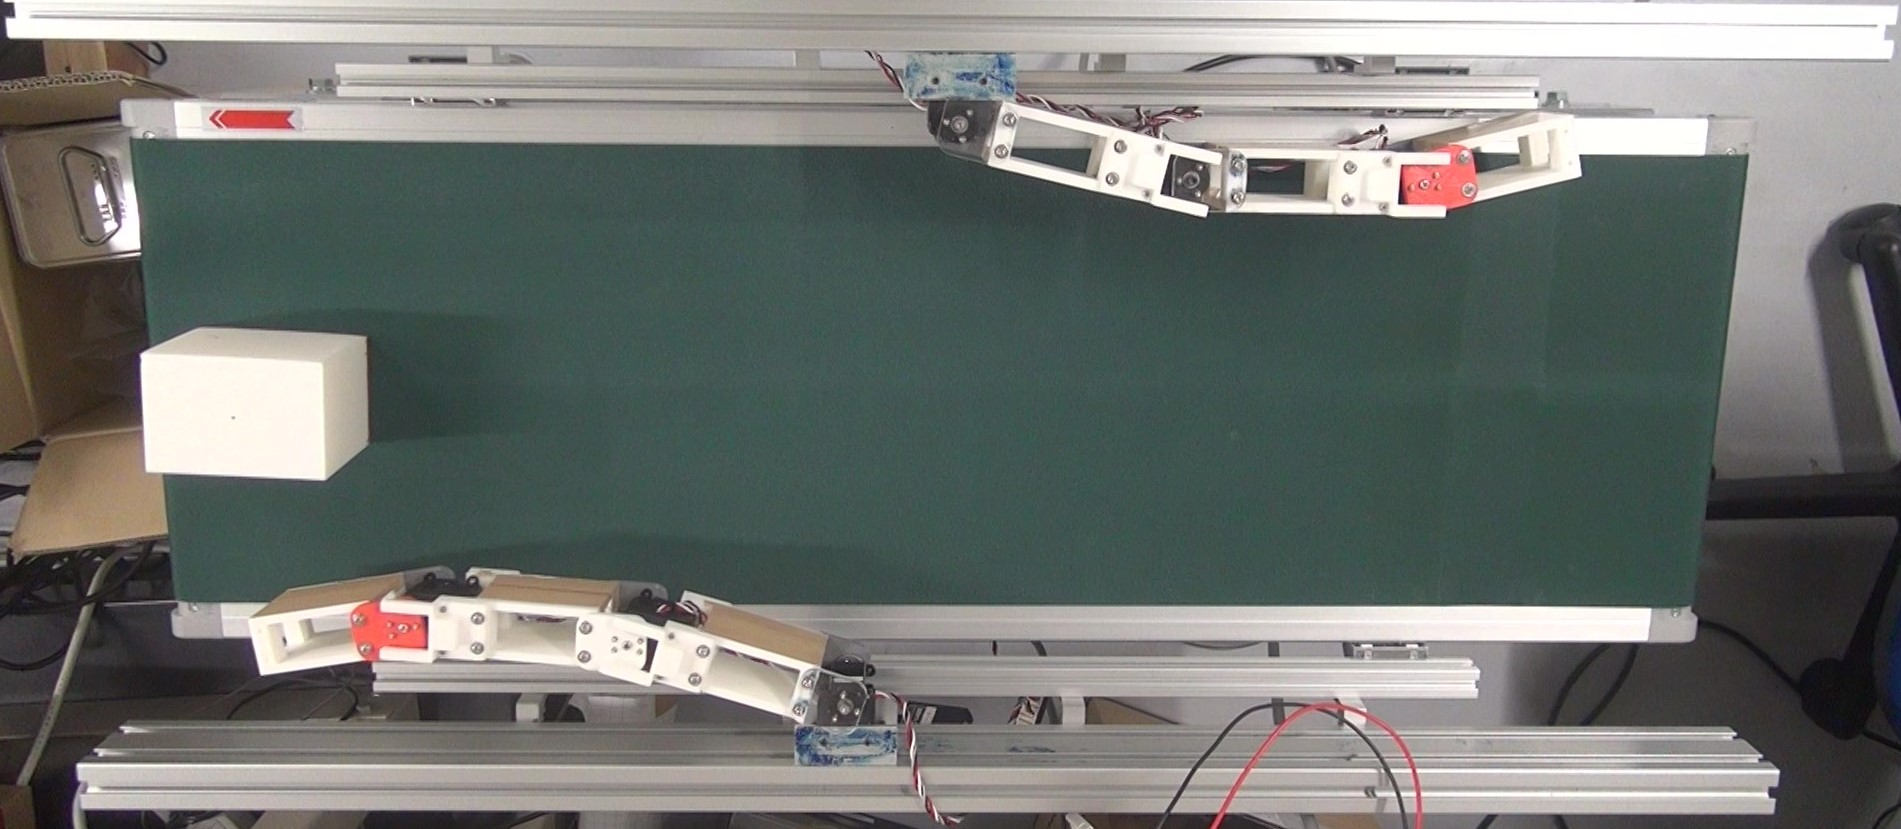
\includegraphics[width=0.98\hsize]{fig/4-manipulation-result/Rectangle/3-6.jpg}
\subcaption{}
\end{minipage}\hfill
\caption{Rectangle alignment as the parts feeder}\label{fig::result::rp}
\end{figure}

\section{三角形のマニピュレーション}
\section{L字形のマニピュレーション}
本節では,L字形物体を対象としたマニピュレーション結果を示す.タスクは,ベルトコンベアに乗って流れてきた対象物を,ベルト幅中央に$0^\circ$で整列させる,というように設定した.動作計画には,両側探索アルゴリズムを用いた.入力情報を以下にまとめる.
\begin{gather}
\notag
\left\{
\begin{aligned}
&ハンド初期姿勢:[\theta_1, \theta_2, \theta_3, \theta_4, \theta_5, \theta_6,] = [40, -50, -30, 40, -50, -30]\mathrm{[deg]}\\
&ハンド最終姿勢:[\theta_1, \theta_2, \theta_3, \theta_4, \theta_5, \theta_6,] = [12, -15, -25, 5, 30, -90]\mathrm{[deg]}\\
&対象物の目標位置・姿勢:[x_{\mathrm {goal}}, y_{\mathrm {goal}}, \phi_{\mathrm {goal}}] = [{\mathrm {any}}, 200 \mathrm{[mm]}, 0 \mathrm{[deg]}]\\
&順探索の終了閾値:\varepsilon = 50\\
&逆探索の終了閾値:\nu = 1000
\end{aligned}
\right .
\end{gather}
動作計画にかかった計算時間は63[s]であり,両探索アルゴリズムの3つの探索終了条件の内,両グラフが結合する終了条件を満たし,経路が生成された.
この経路を用いてL字形物体の異なる2つの初期位置・姿勢に対してマニピュレーションを行った.結果を\figref{fig::result::lm1},\figref{fig::result::lm2}に示す.
\begin{figure}[hbt]
\centering
\begin{minipage}{0.249\hsize}
\centering
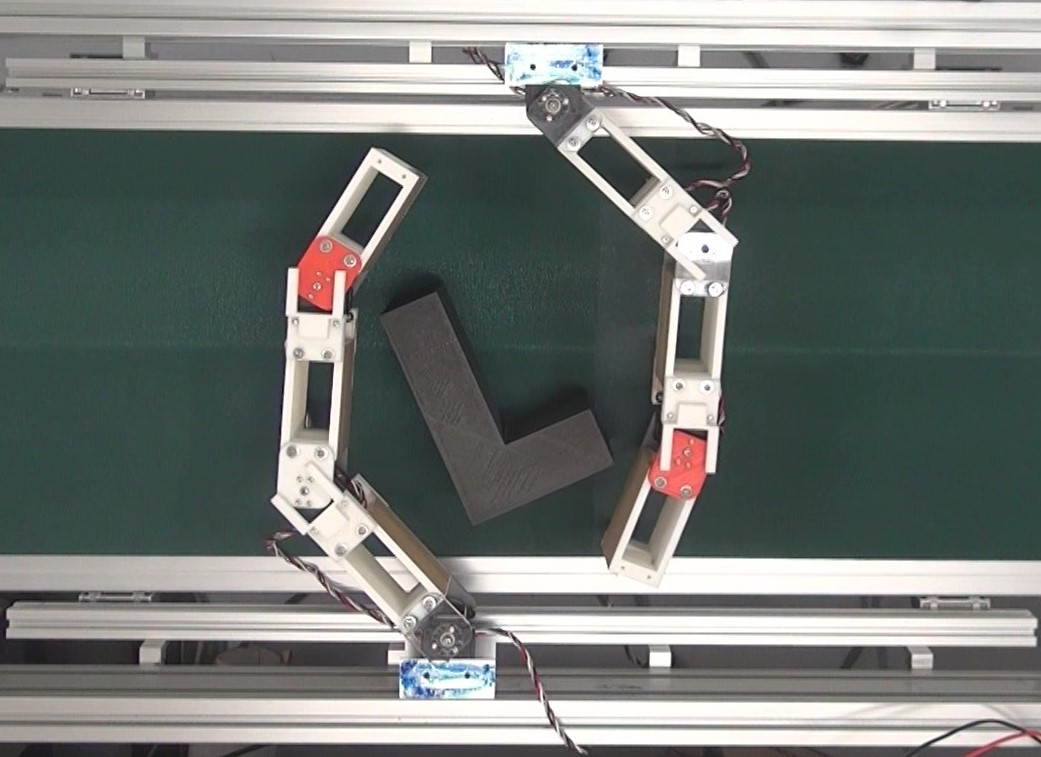
\includegraphics[width=0.98\hsize]{fig/4-manipulation-result/LShape/1-1.jpg}
\subcaption{}\label{}
\end{minipage}\hfill
\begin{minipage}{0.249\hsize}
\centering
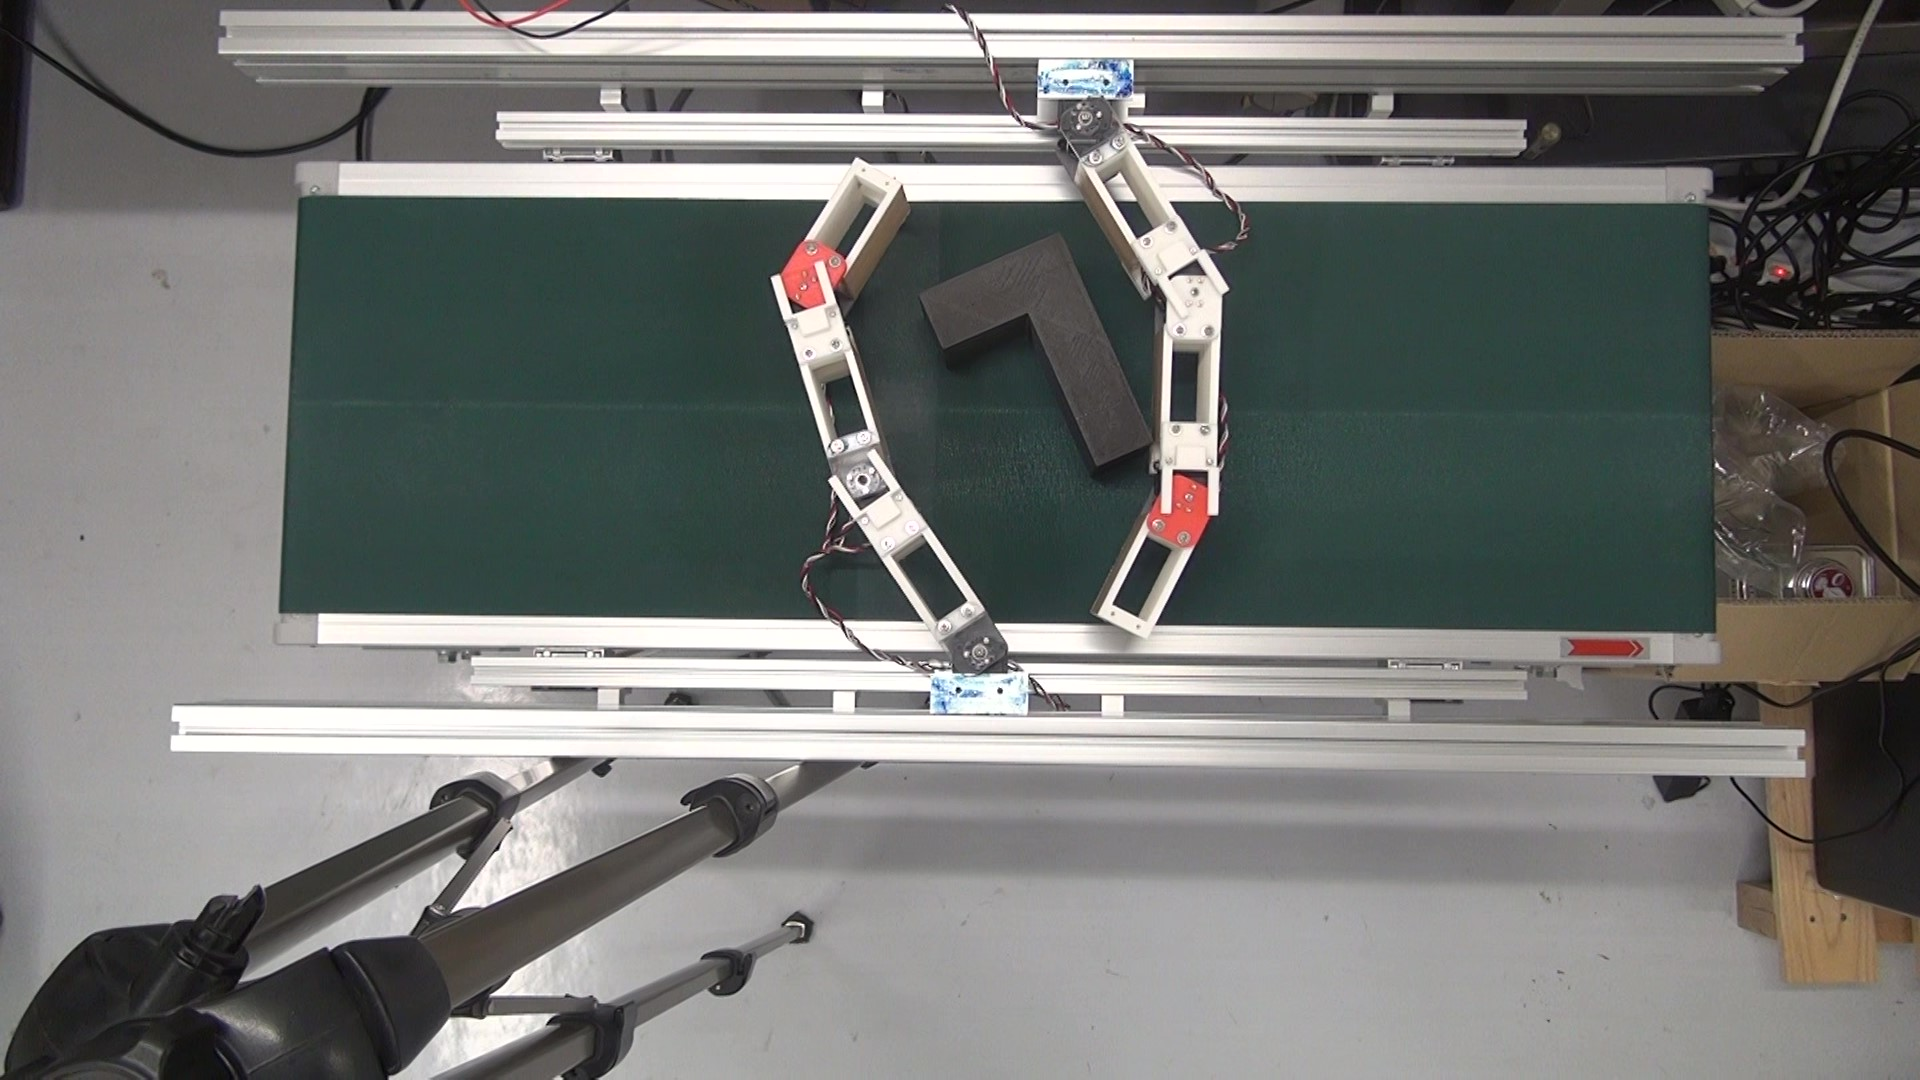
\includegraphics[width=0.98\hsize]{fig/4-manipulation-result/LShape/1-2.jpg}
\subcaption{}\label{}
\end{minipage}\hfill
\begin{minipage}{0.249\hsize}
\centering
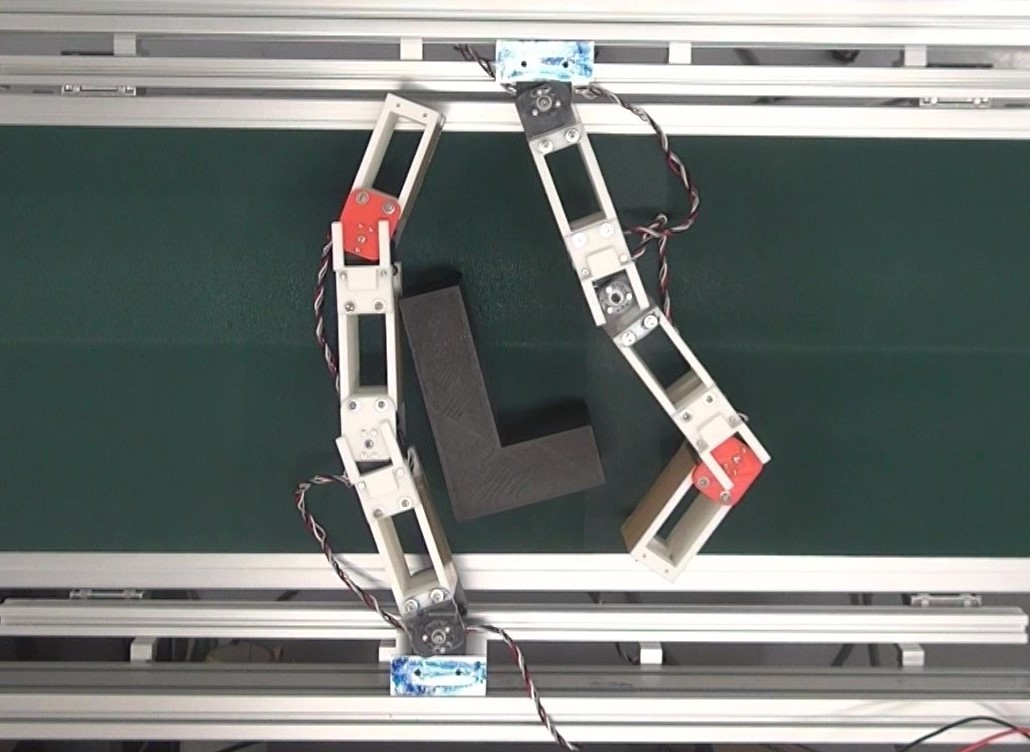
\includegraphics[width=0.98\hsize]{fig/4-manipulation-result/LShape/1-3.jpg}
\subcaption{}\label{}
\end{minipage}\hfill
\begin{minipage}{0.249\hsize}
\centering
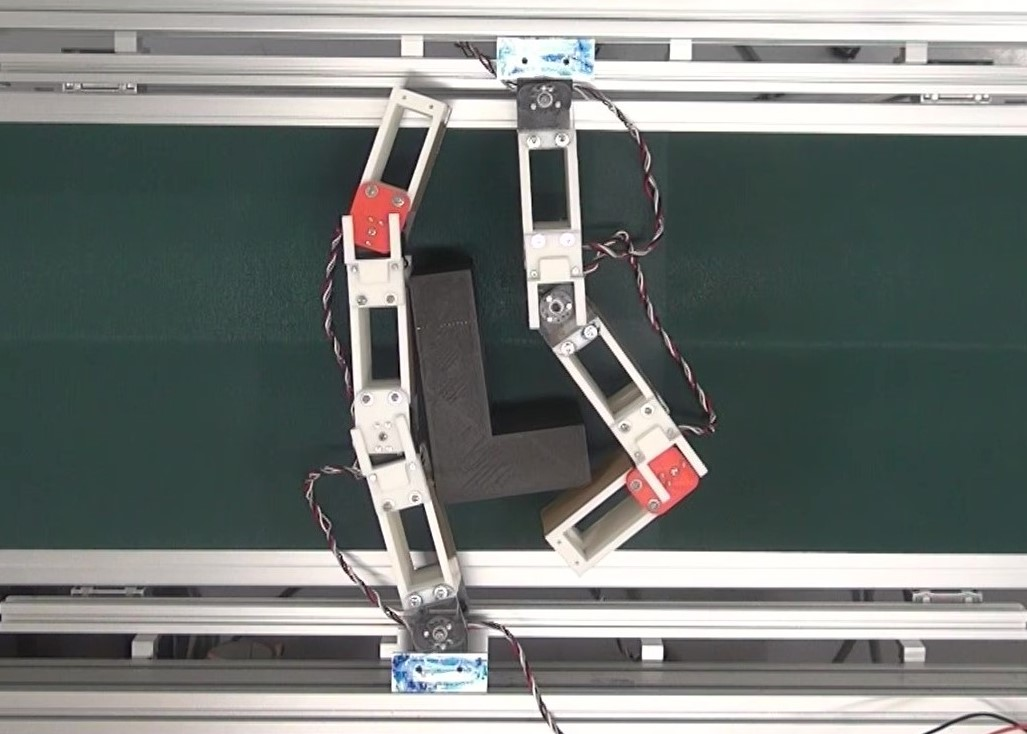
\includegraphics[width=0.98\hsize]{fig/4-manipulation-result/LShape/1-4.jpg}
\subcaption{}\label{}
\end{minipage}
\caption{LShape manipulation result \#1}\label{fig::result::lm1}
\end{figure}

\begin{figure}[hbt]
\centering
\begin{minipage}{0.249\hsize}
\centering
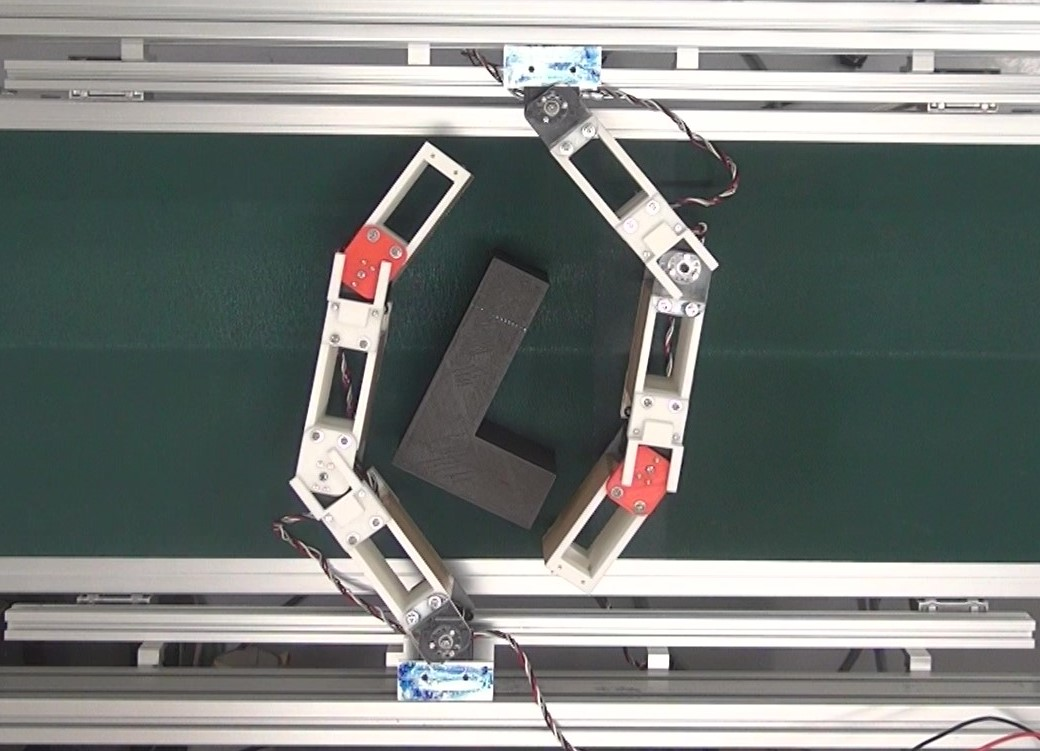
\includegraphics[width=0.98\hsize]{fig/4-manipulation-result/LShape/2-1.jpg}
\subcaption{}\label{}
\end{minipage}\hfill
\begin{minipage}{0.249\hsize}
\centering
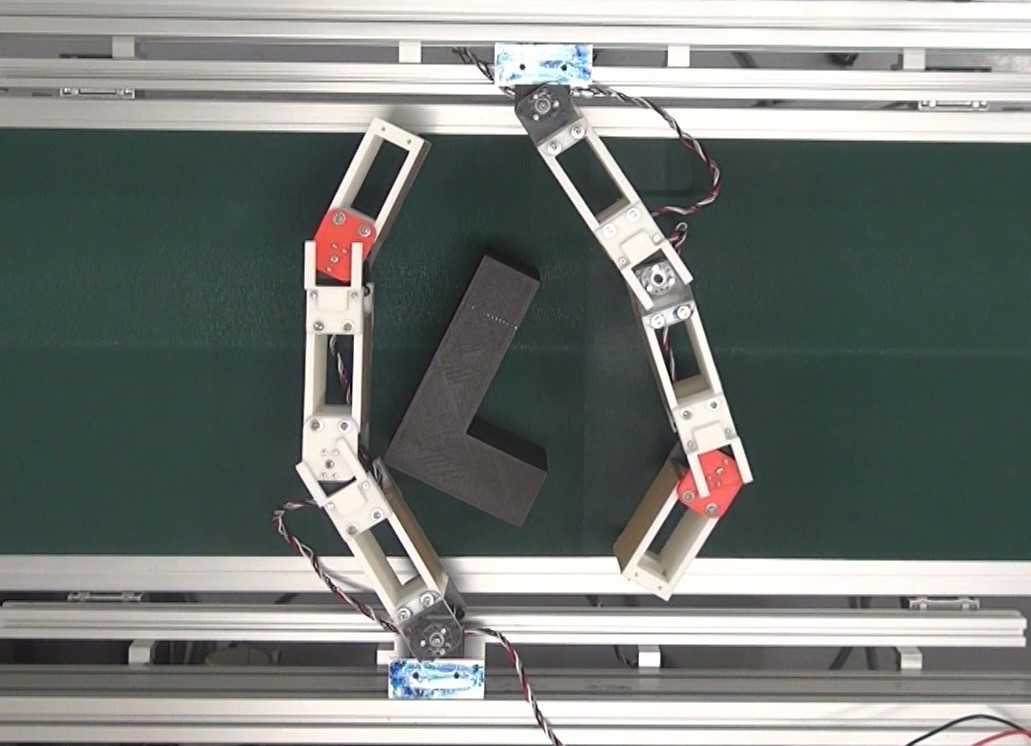
\includegraphics[width=0.98\hsize]{fig/4-manipulation-result/LShape/2-2.jpg}
\subcaption{}\label{}
\end{minipage}\hfill
\begin{minipage}{0.249\hsize}
\centering
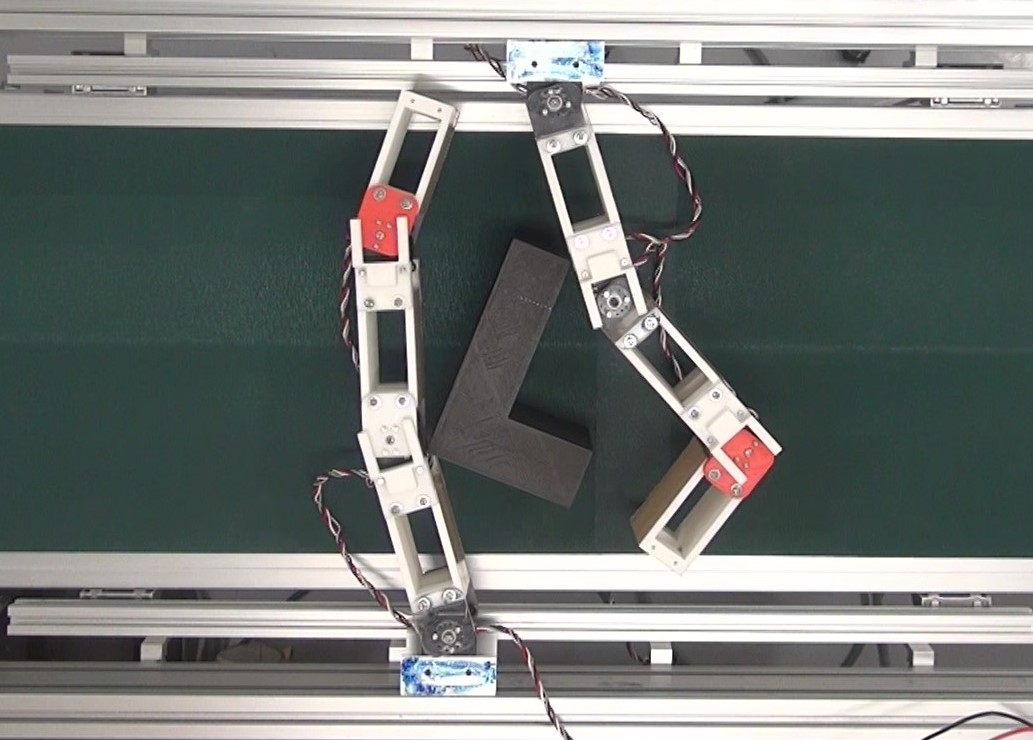
\includegraphics[width=0.98\hsize]{fig/4-manipulation-result/LShape/2-3.jpg}
\subcaption{}\label{}
\end{minipage}\hfill
\begin{minipage}{0.249\hsize}
\centering
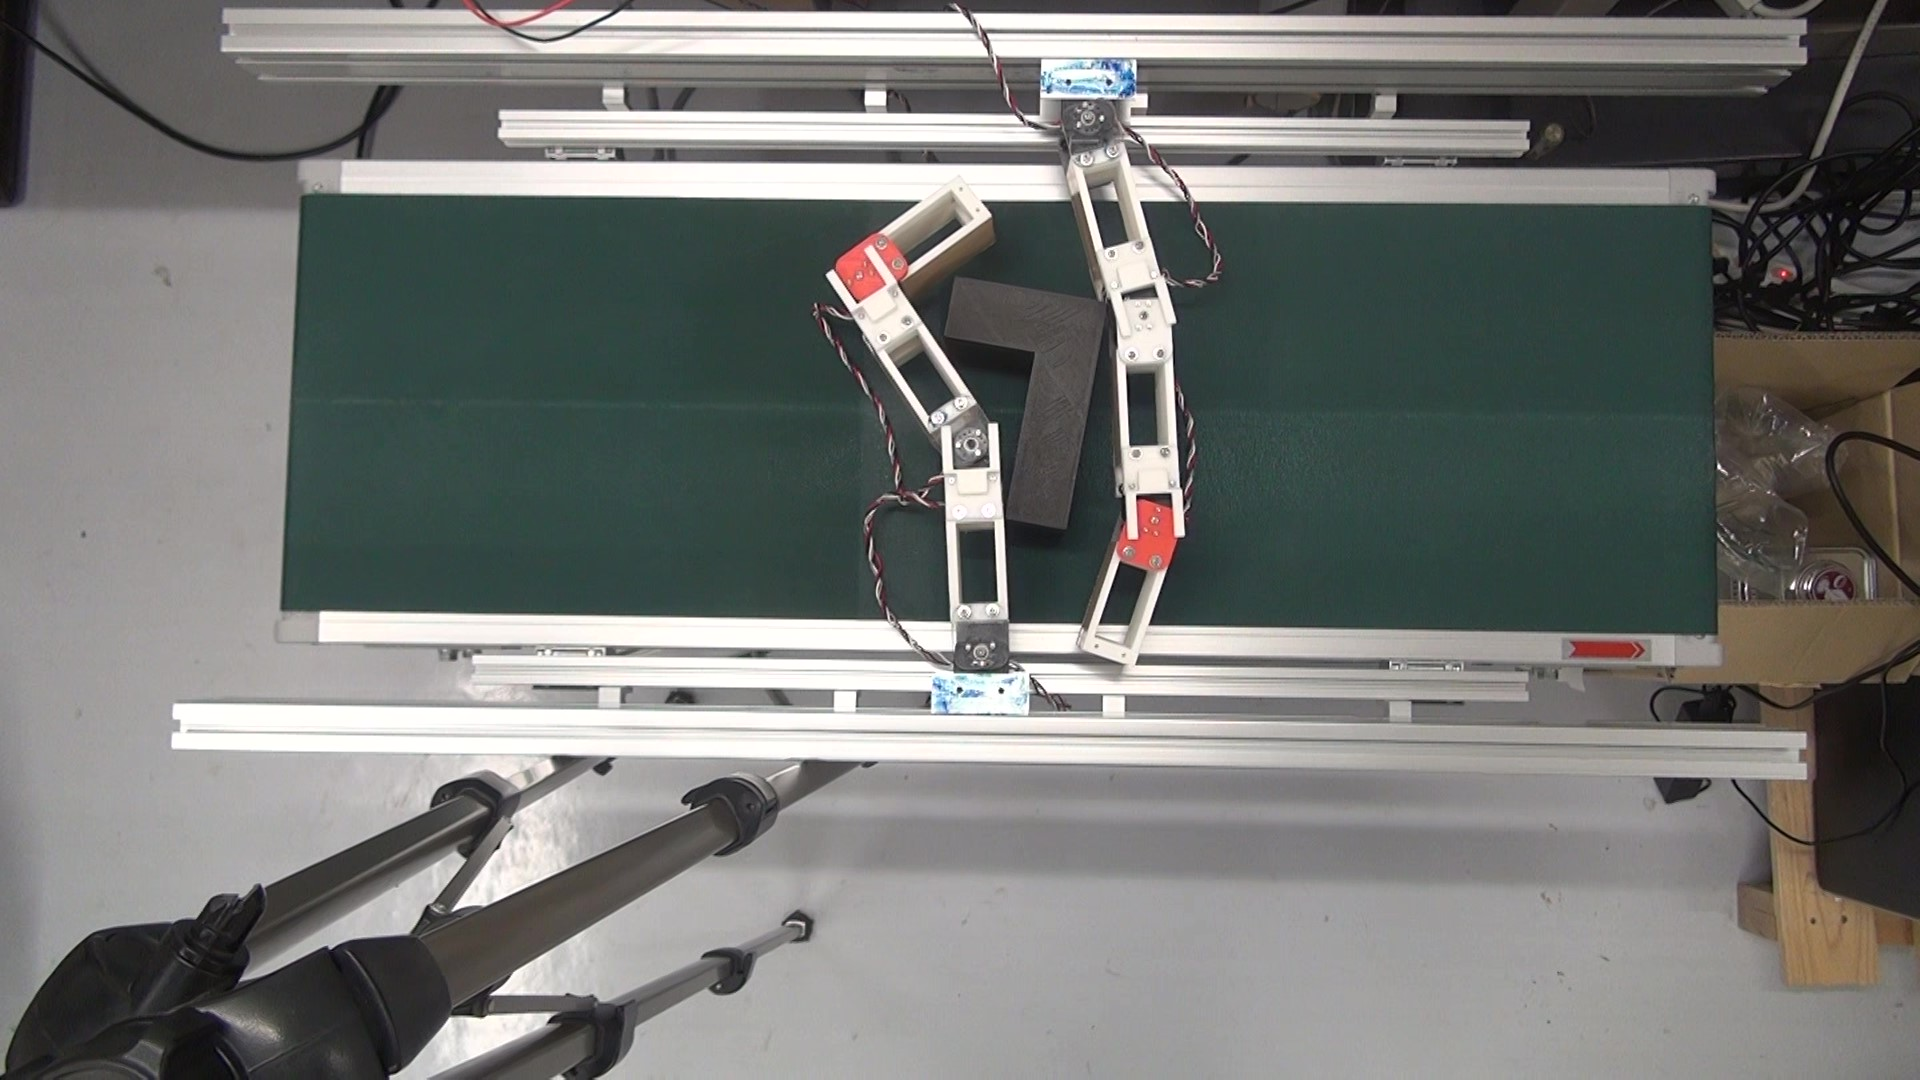
\includegraphics[width=0.98\hsize]{fig/4-manipulation-result/LShape/2-4.jpg}
\subcaption{}\label{}
\end{minipage}
\caption{LShape manipulation result \#2}\label{fig::result::lm2}
\end{figure}

\figref{fig::result::lm1}のマニピュレーション後の対象物位置・姿勢は,$(x, y, \phi) = (\_, 202 \mathrm{[mm]}, 7 \mathrm{[deg]})$であり,目標位置・姿勢から$\Delta y = +2 \mathrm{[mm]}$,$\Delta \phi = +7 \mathrm{[deg]}$の誤差があった.また,\figref{fig::result::lm2}のマニピュレーション後の対象物位置・姿勢は,$(x, y, \phi) = (\_, 212 \mathrm{[mm]}, -9 \mathrm{[deg]})$であり,目標位置・姿勢から$\Delta y = +12 \mathrm{[mm]}$,$\Delta \phi = -9 \mathrm{[deg]}$の誤差があった.\par

次に,パーツフィーダとしての動作結果を\figref{fig::result::lp}に示す.これより,L字形物体に対してキャッチ,整列,リリースの一連のタスクを行えることを確認した.
\begin{figure}[hb]
\centering
\begin{minipage}{0.49\hsize}
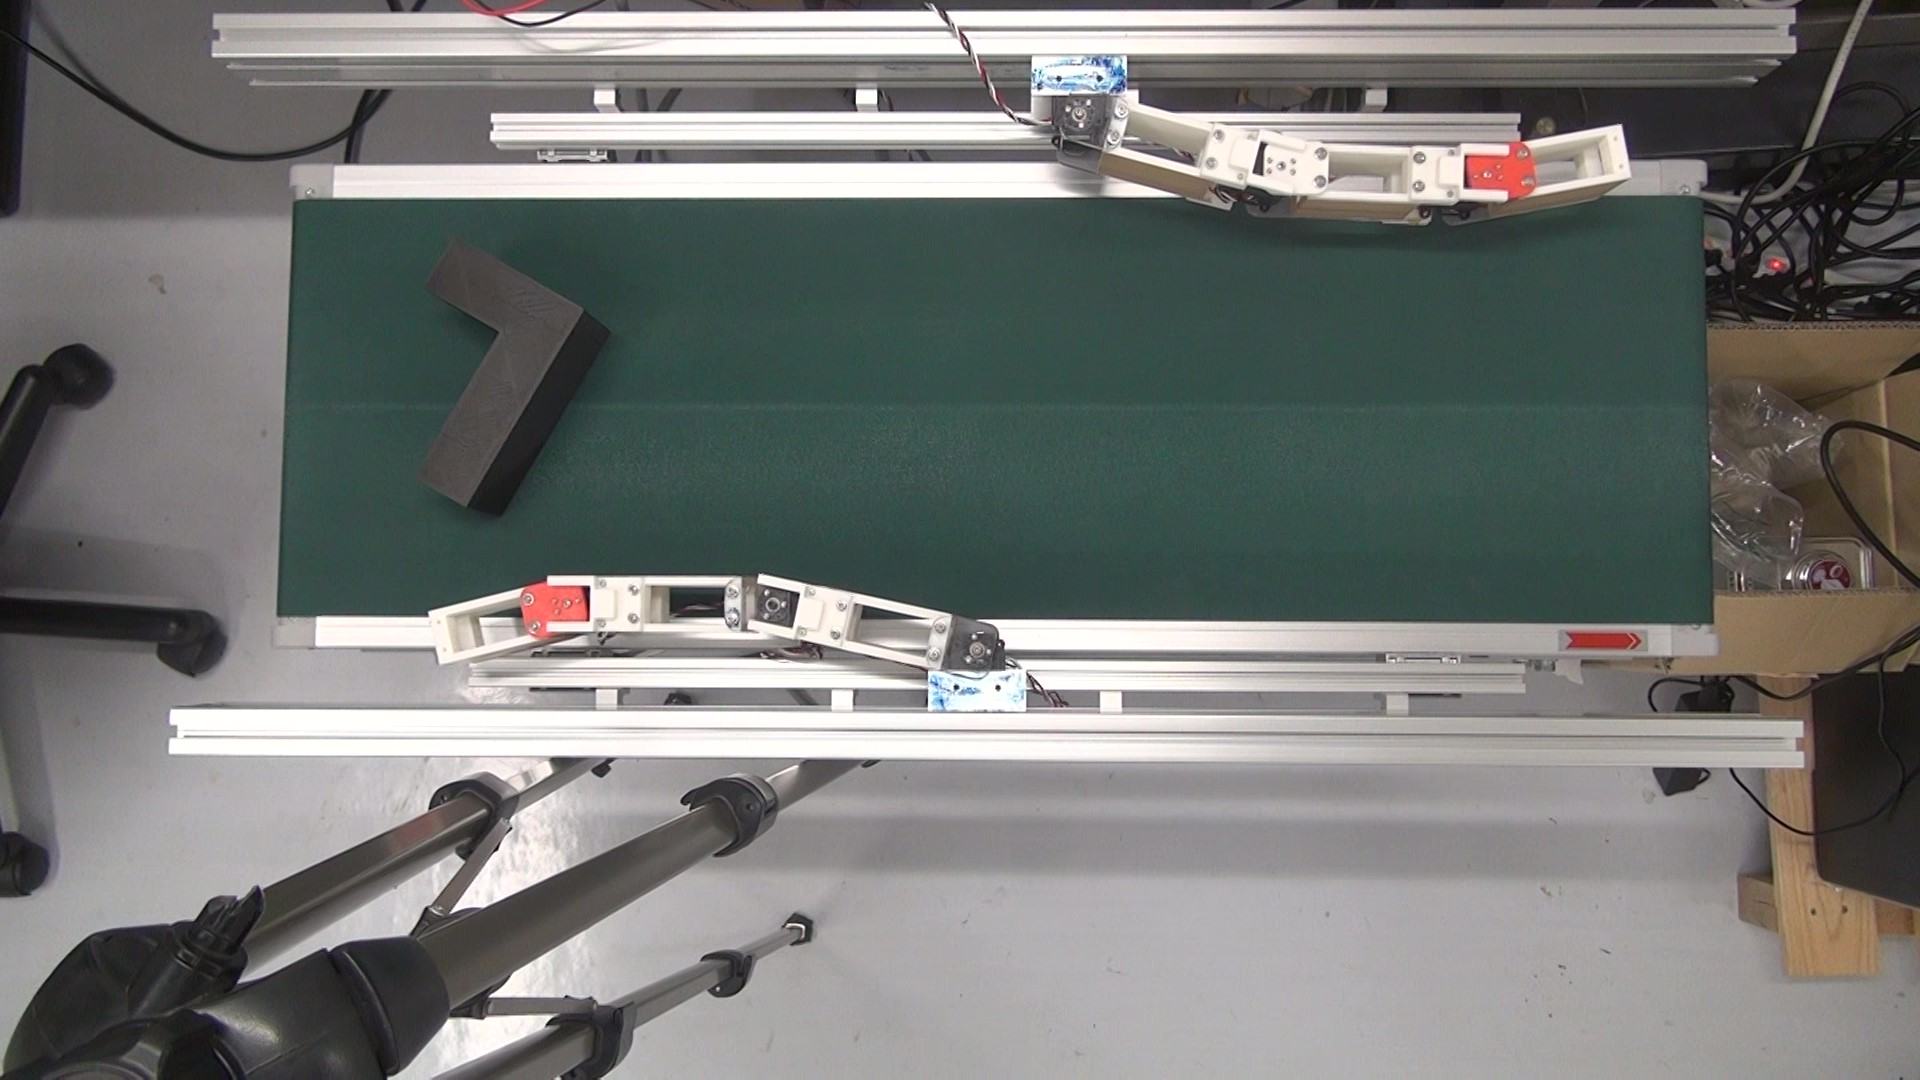
\includegraphics[width=0.98\hsize]{fig/4-manipulation-result/LShape/3-1.jpg}
\subcaption{}
\end{minipage}\hfill
\begin{minipage}{0.49\hsize}
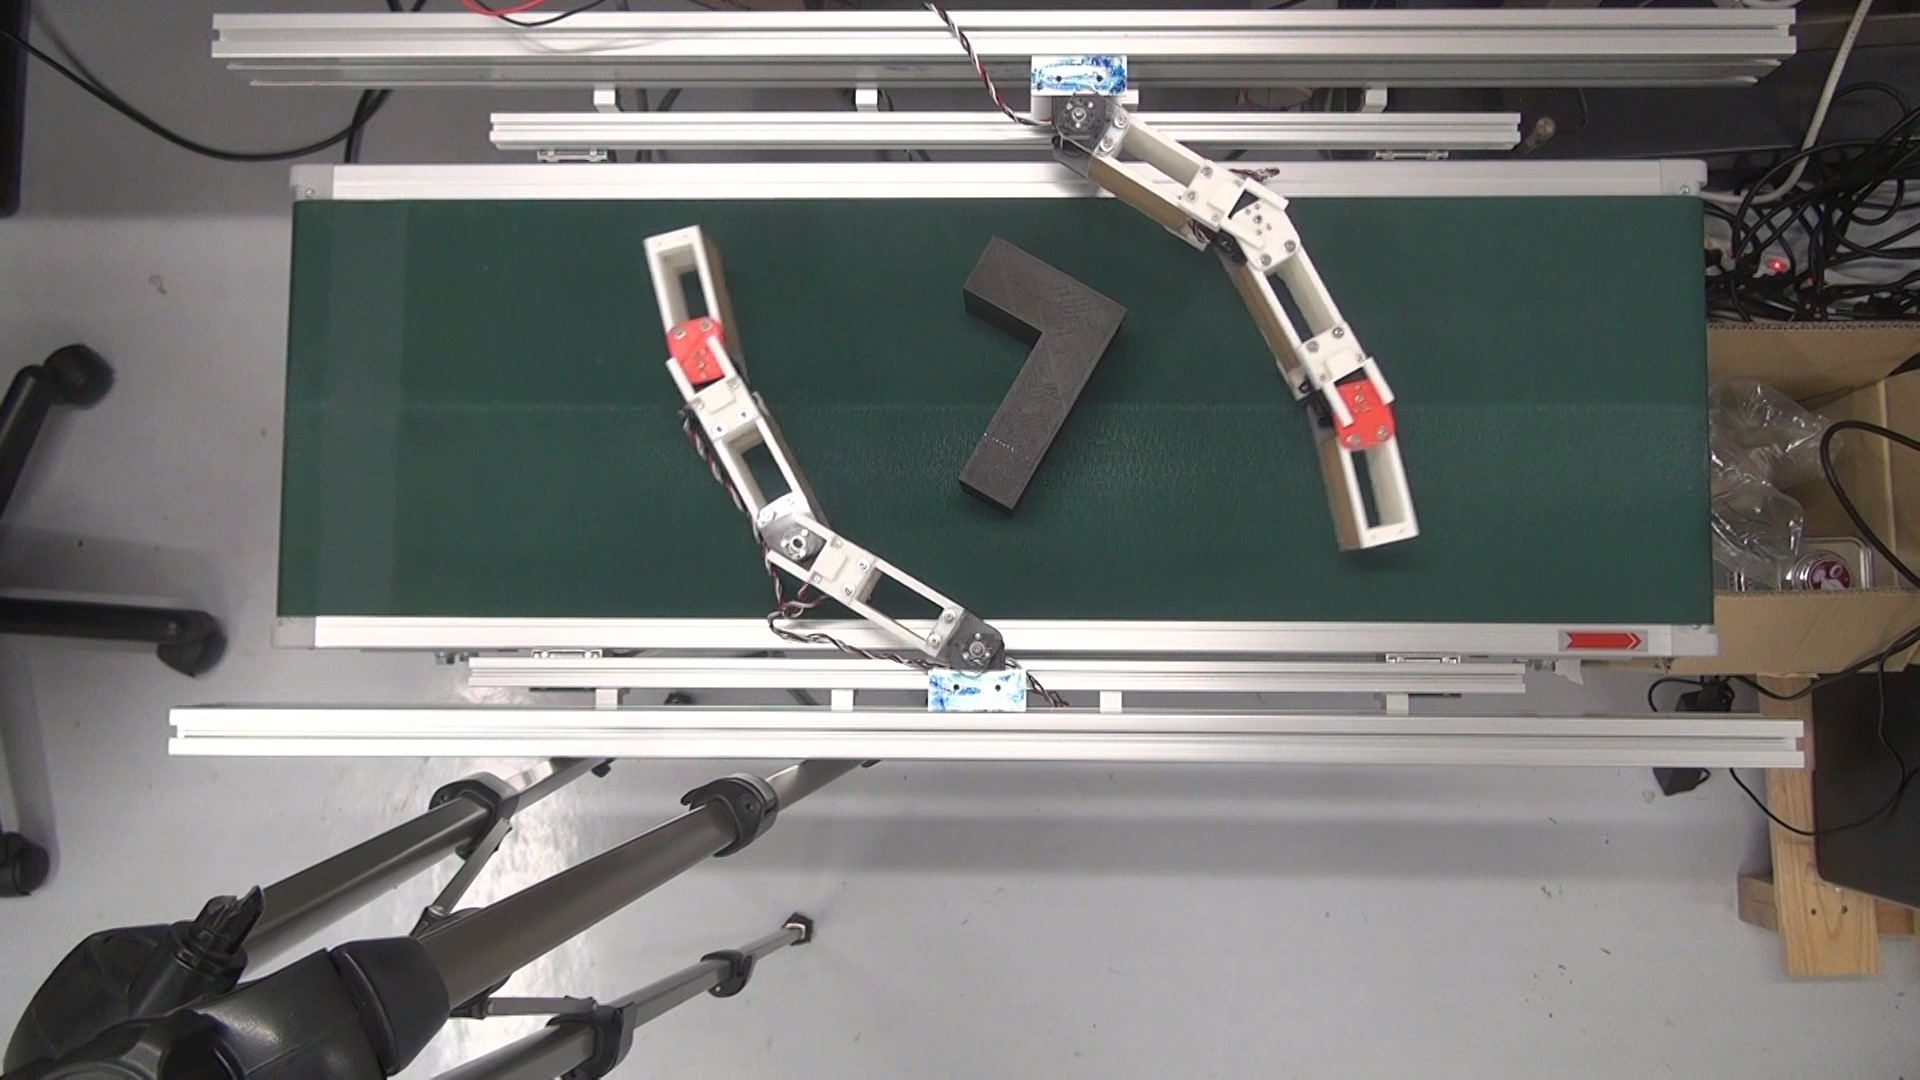
\includegraphics[width=0.98\hsize]{fig/4-manipulation-result/LShape/3-2.jpg}
\subcaption{}
\end{minipage}\hfill
\begin{minipage}{0.49\hsize}
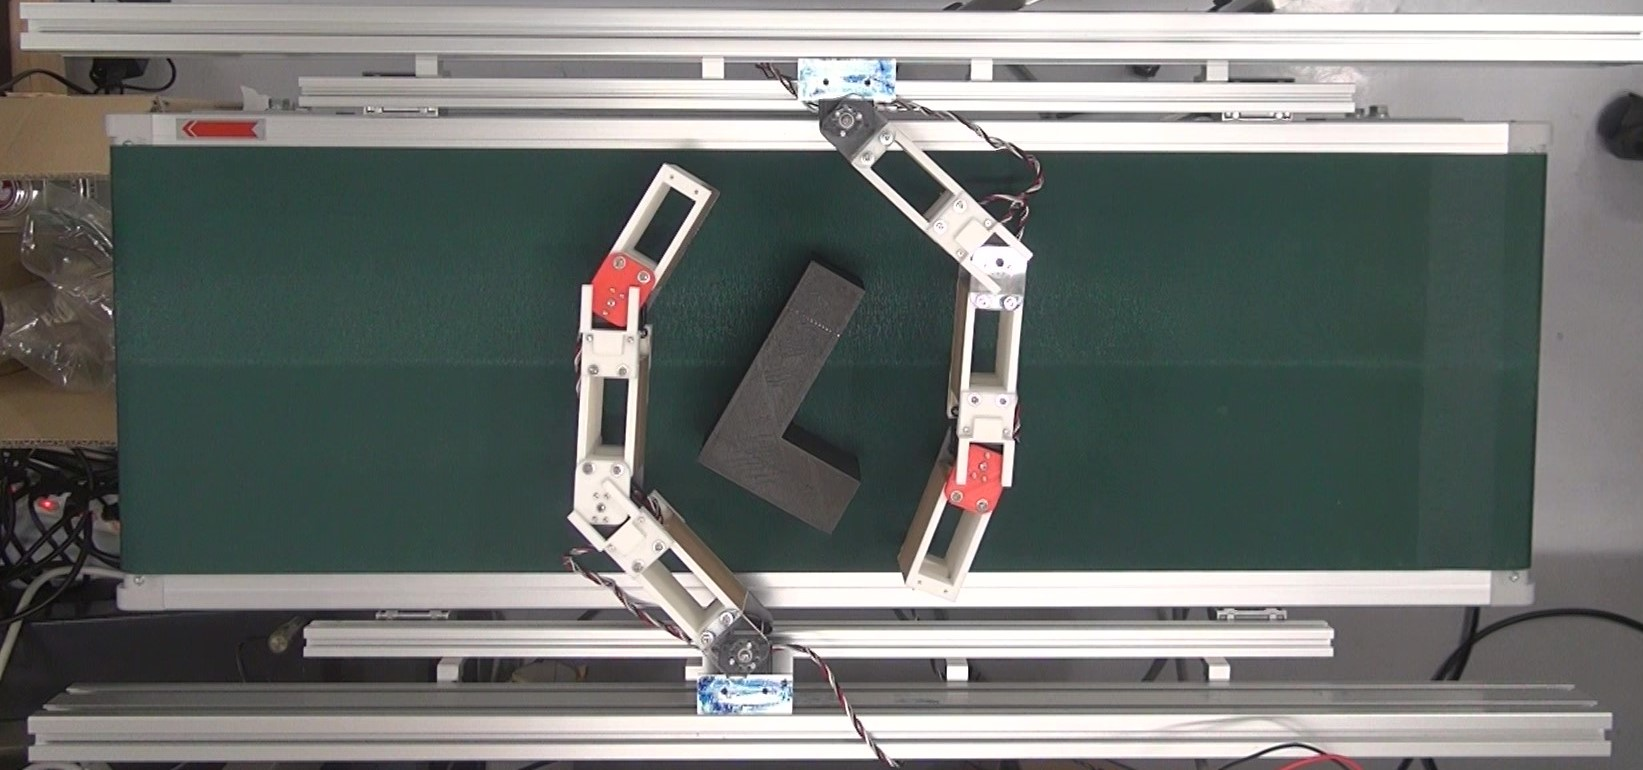
\includegraphics[width=0.98\hsize]{fig/4-manipulation-result/LShape/3-3.jpg}
\subcaption{}
\end{minipage}\hfill
\begin{minipage}{0.49\hsize}
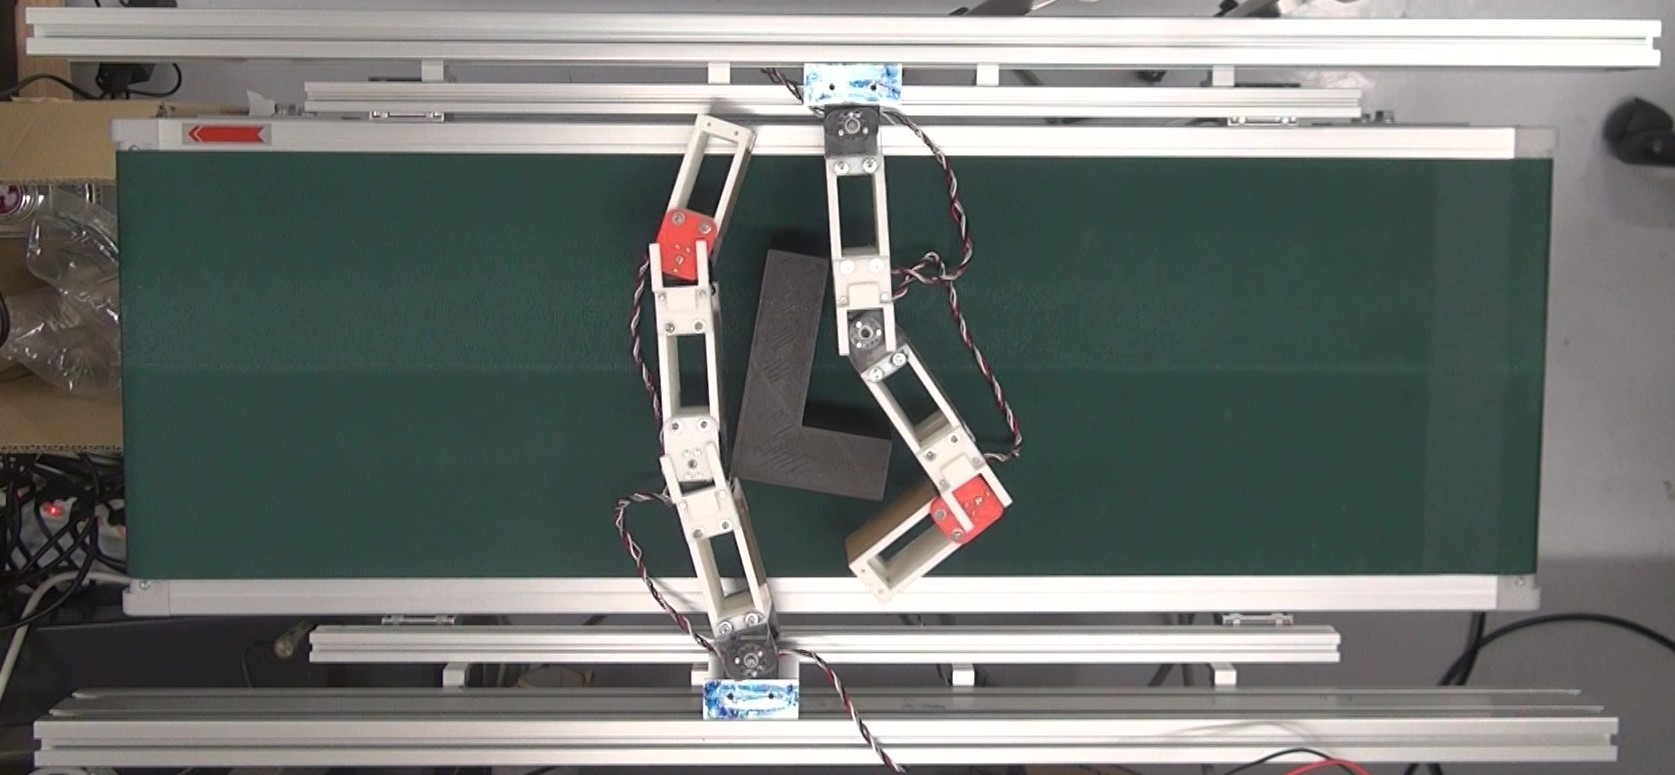
\includegraphics[width=0.98\hsize]{fig/4-manipulation-result/LShape/3-4.jpg}
\subcaption{}
\end{minipage}\hfill
\begin{minipage}{0.49\hsize}
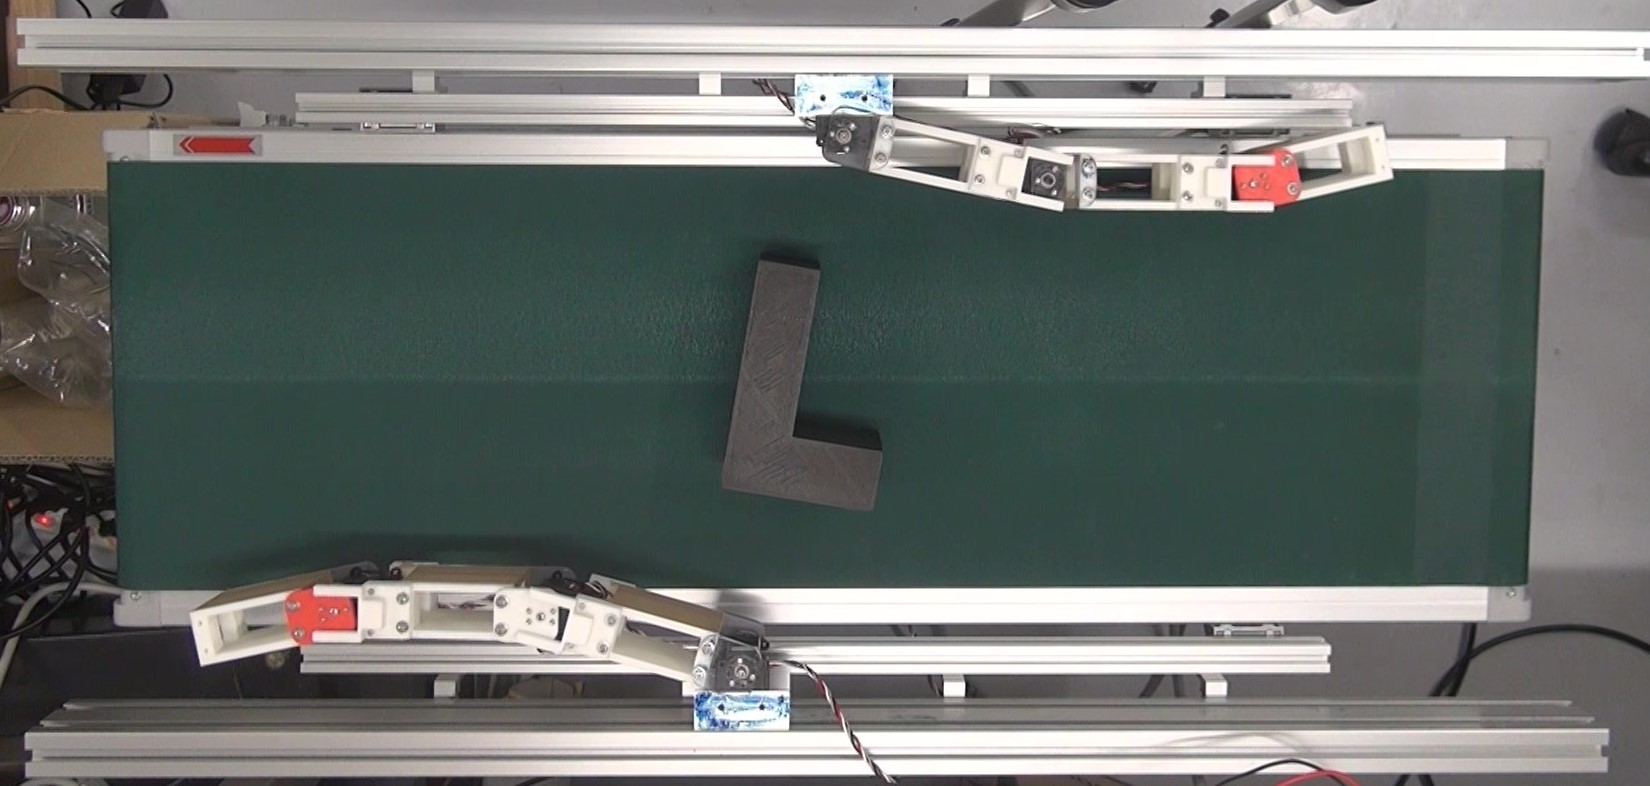
\includegraphics[width=0.98\hsize]{fig/4-manipulation-result/LShape/3-5.jpg}
\subcaption{}
\end{minipage}\hfill
\begin{minipage}{0.49\hsize}
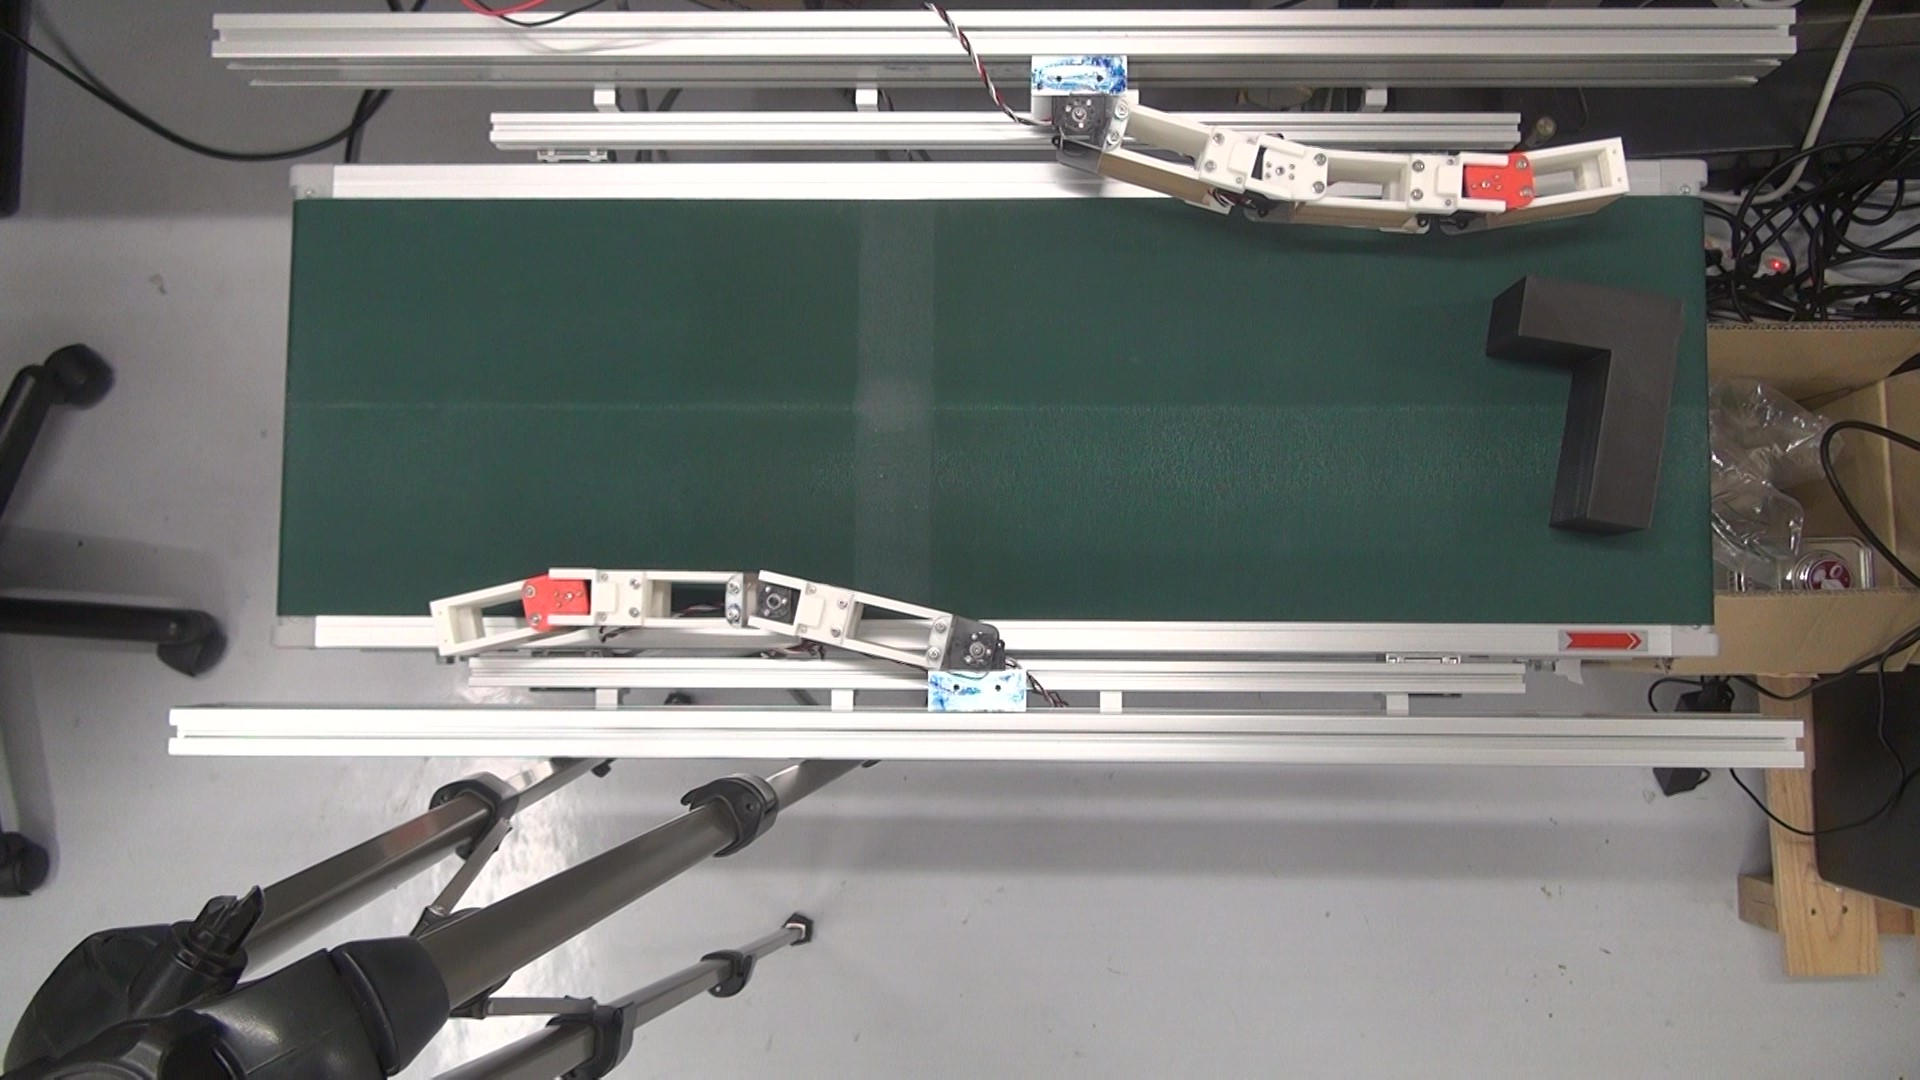
\includegraphics[width=0.98\hsize]{fig/4-manipulation-result/LShape/3-6.jpg}
\subcaption{}
\end{minipage}\hfill
\caption{LShape alignment as the parts feeder}\label{fig::result::lp}
\end{figure}

\section{T字形のマニピュレーション}
本節では,T字形物体を対象としたマニピュレーション結果を示す.タスクは,ベルトコンベアに乗って流れてきた対象物を,ベルト幅中央に$0^\circ$で整列させる,というように設定した.動作計画には,両側探索アルゴリズムを用いた.入力情報を以下にまとめる.
\begin{gather}
\notag
\left\{
\begin{aligned}
&ハンド初期姿勢:[\theta_1, \theta_2, \theta_3, \theta_4, \theta_5, \theta_6,] = [36, -30, -33, 25, -15, -31]\mathrm{[deg]}\\
&ハンド最終姿勢:[\theta_1, \theta_2, \theta_3, \theta_4, \theta_5, \theta_6,] = [19.2, -21.8, -80.6, 20.8, -36.2, -9.02]\mathrm{[deg]}\\
&対象物の目標位置・姿勢:[x_{\mathrm {goal}}, y_{\mathrm {goal}}, \phi_{\mathrm {goal}}] = [{\mathrm {any}}, 200 \mathrm{[mm]}, 0 \mathrm{[deg]}]\\
&順探索の終了閾値:\varepsilon = 50\\
&逆探索の終了閾値:\nu = 800
\end{aligned}
\right .
\end{gather}
動作計画にかかった計算時間は3.9[s]であり,両探索アルゴリズムの3つの探索終了条件の内,両グラフが結合する終了条件を満たし,経路が生成された.
この経路を用いてT字形物体の異なる2つの初期位置・姿勢に対してマニピュレーションを行った.
結果を\figref{fig::result::tm1},\figref{fig::result::tm2}に示す.
\begin{figure}[hbt]
\centering
\begin{minipage}{0.249\hsize}
\centering
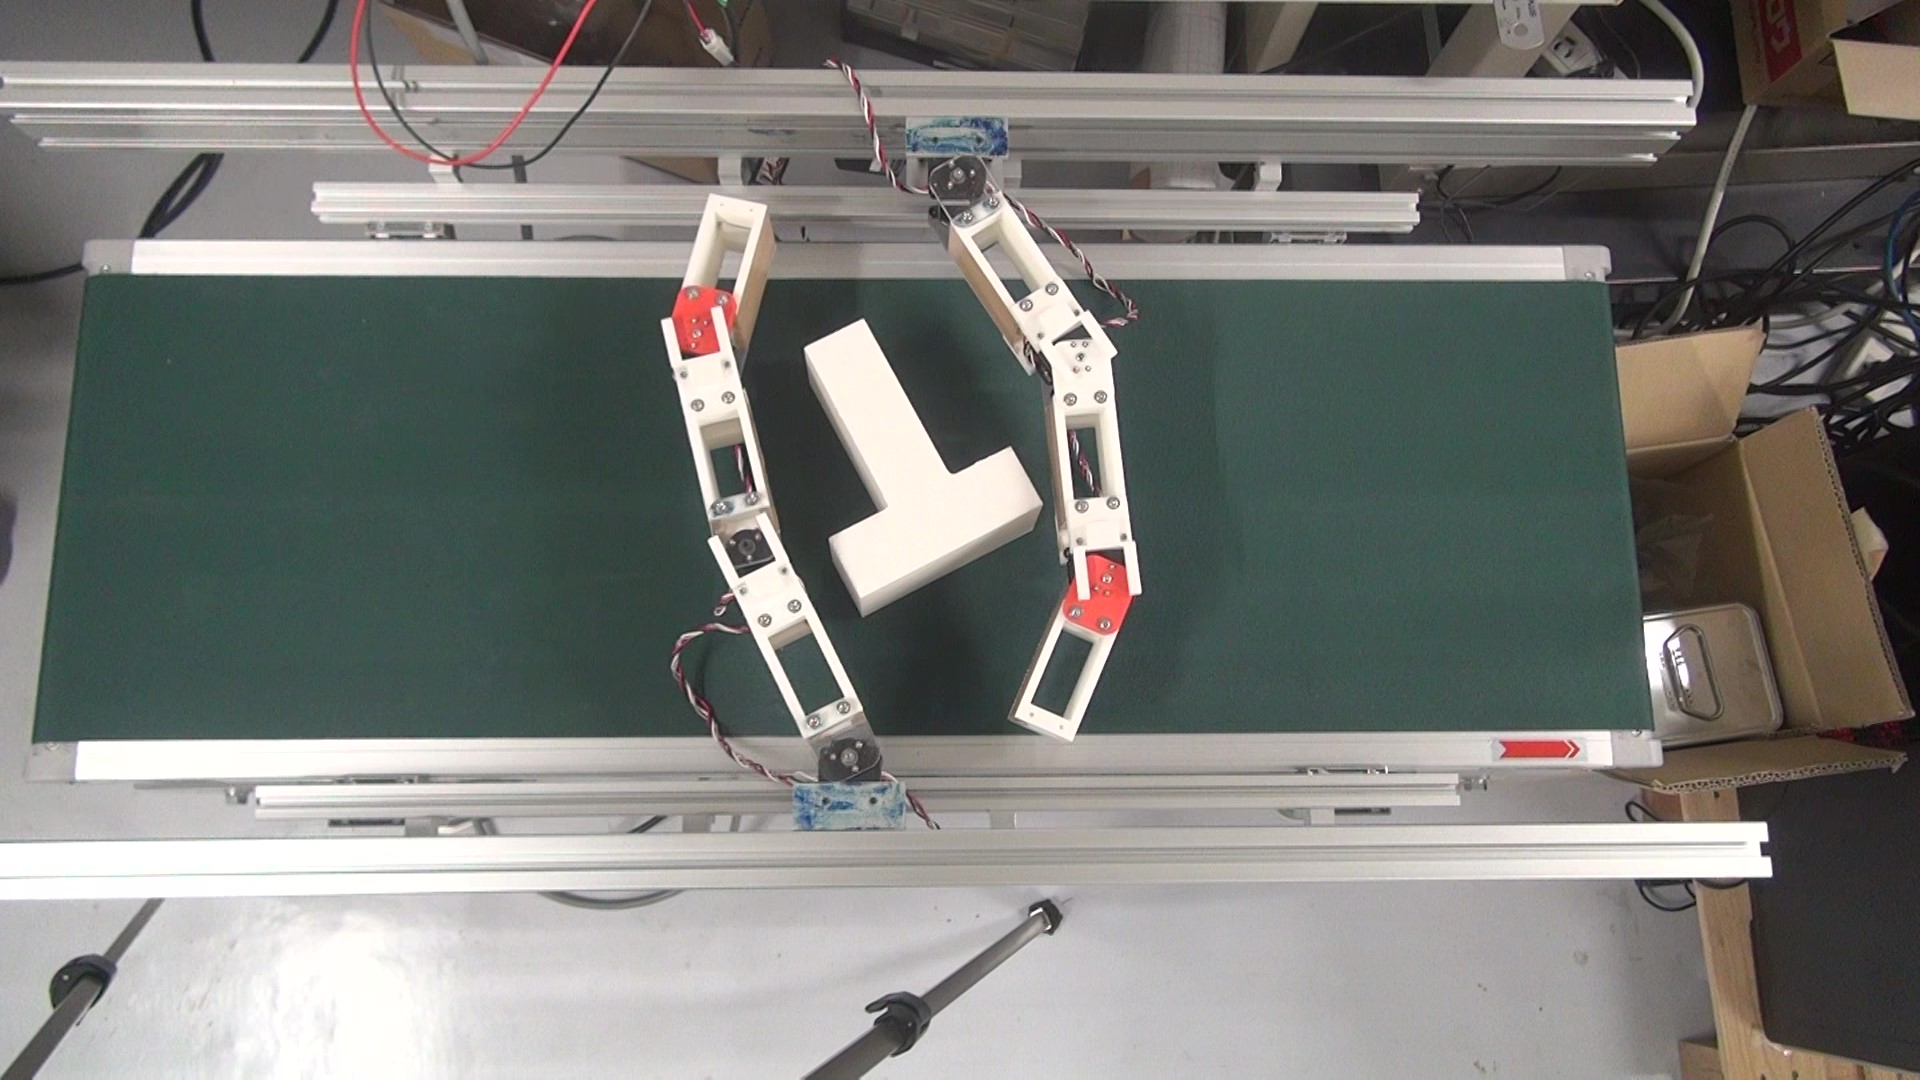
\includegraphics[width=0.98\hsize]{fig/4-manipulation-result/TShape/1-1.jpg}
\subcaption{}\label{}
\end{minipage}\hfill
\begin{minipage}{0.249\hsize}
\centering
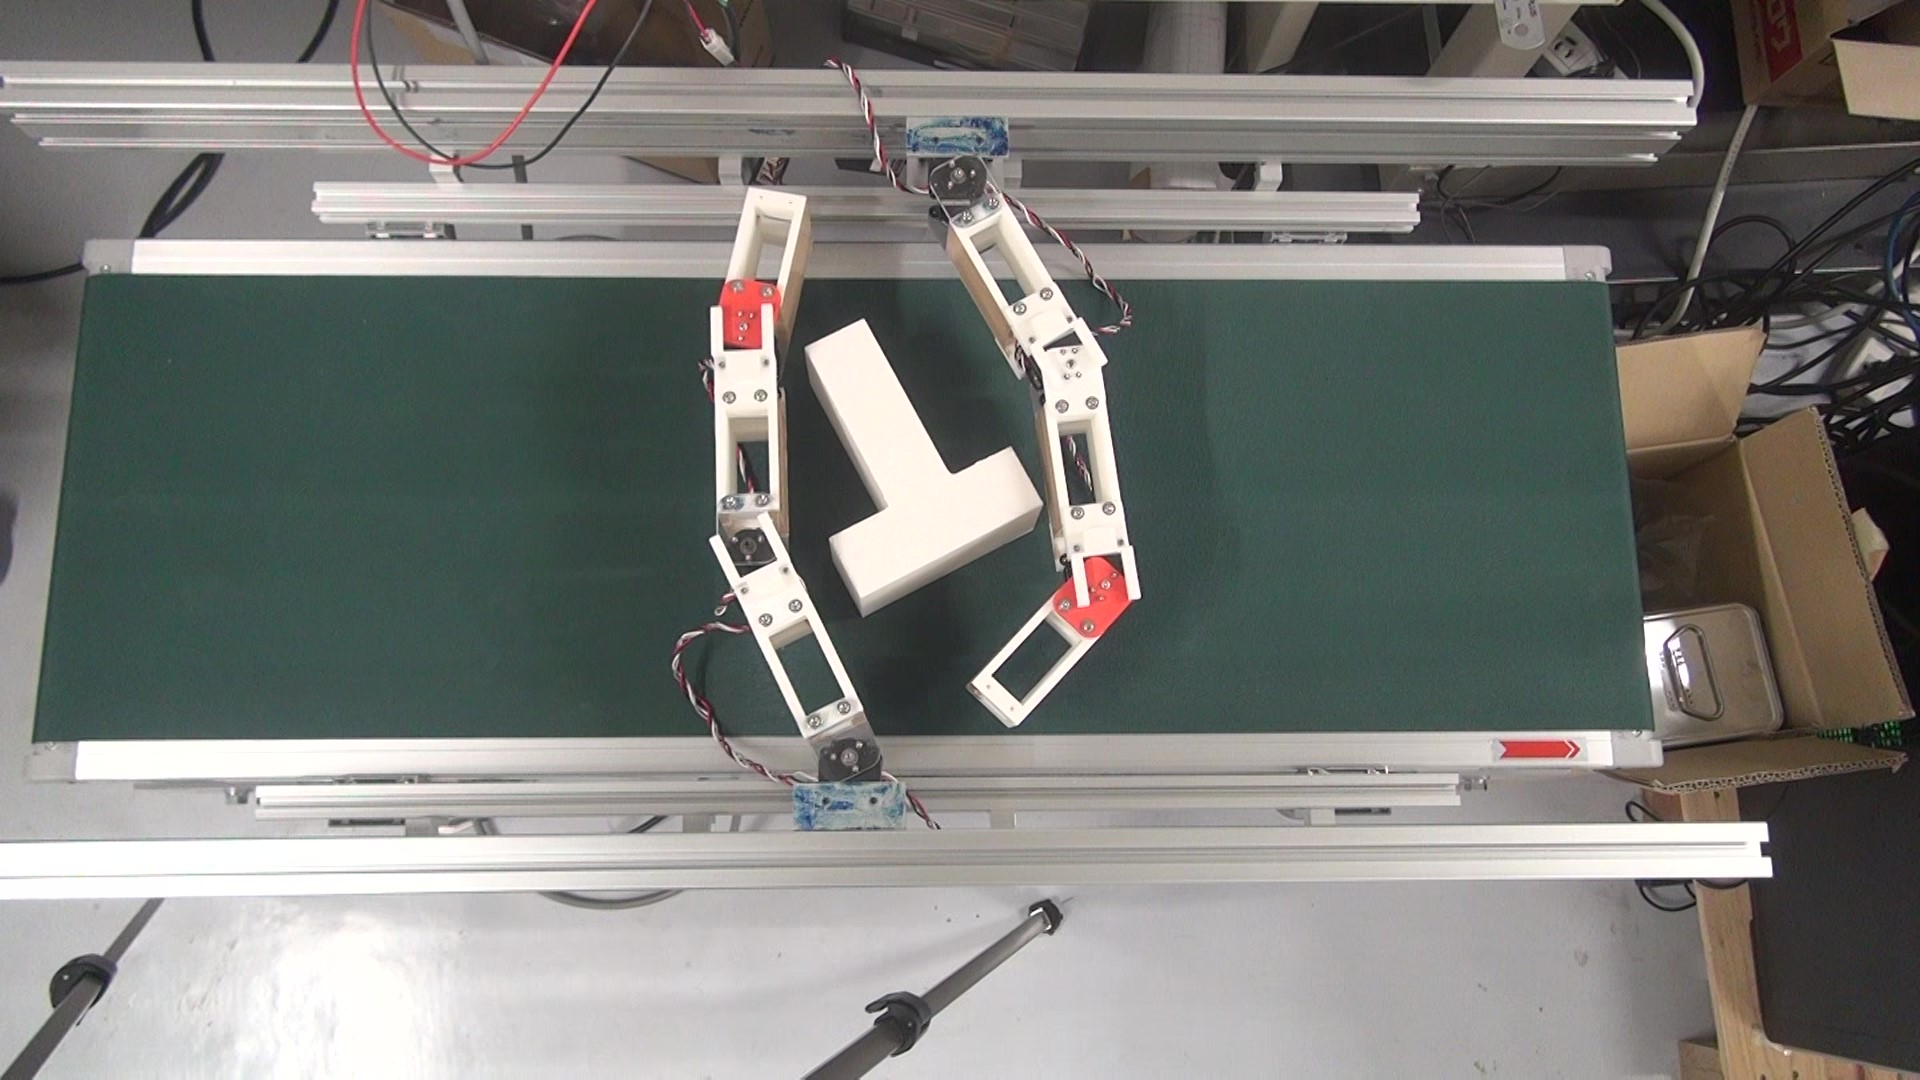
\includegraphics[width=0.98\hsize]{fig/4-manipulation-result/TShape/1-2.jpg}
\subcaption{}\label{}
\end{minipage}\hfill
\begin{minipage}{0.249\hsize}
\centering
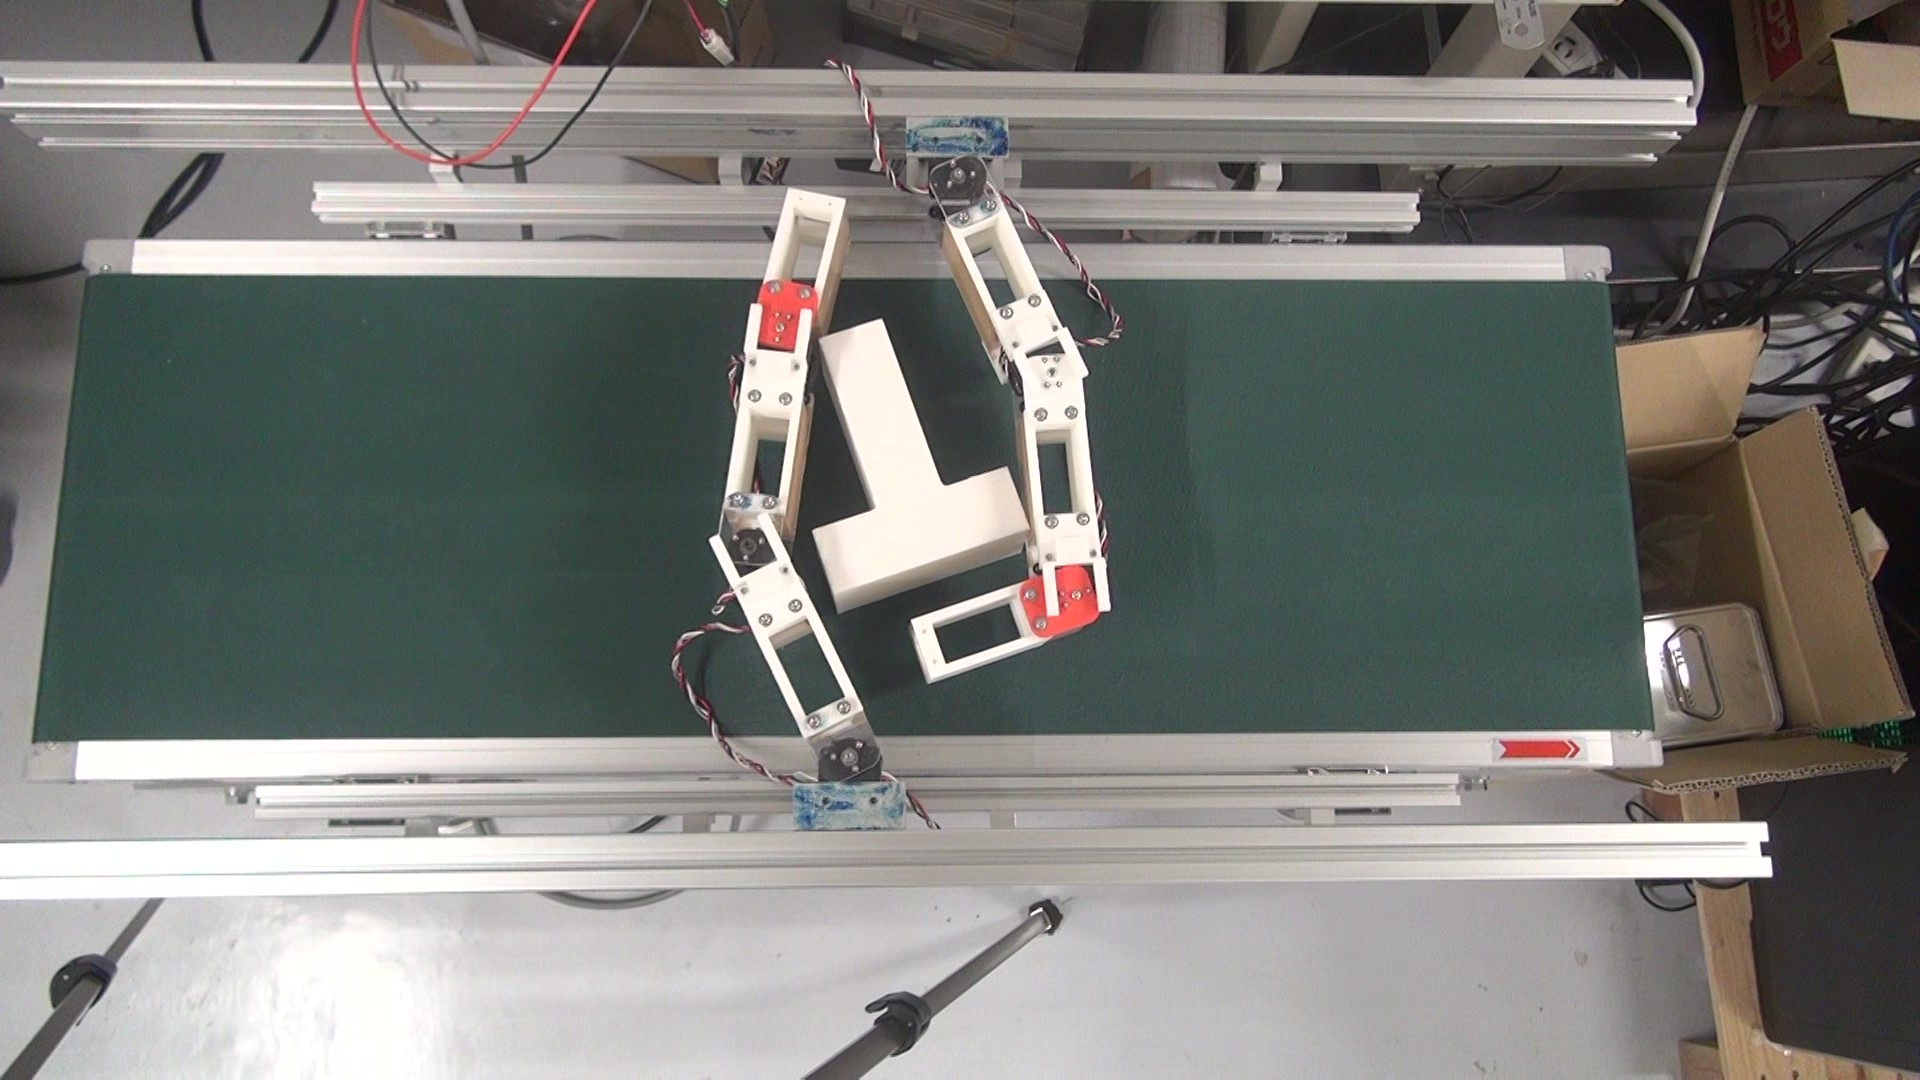
\includegraphics[width=0.98\hsize]{fig/4-manipulation-result/TShape/1-3.jpg}
\subcaption{}\label{}
\end{minipage}\hfill
\begin{minipage}{0.249\hsize}
\centering
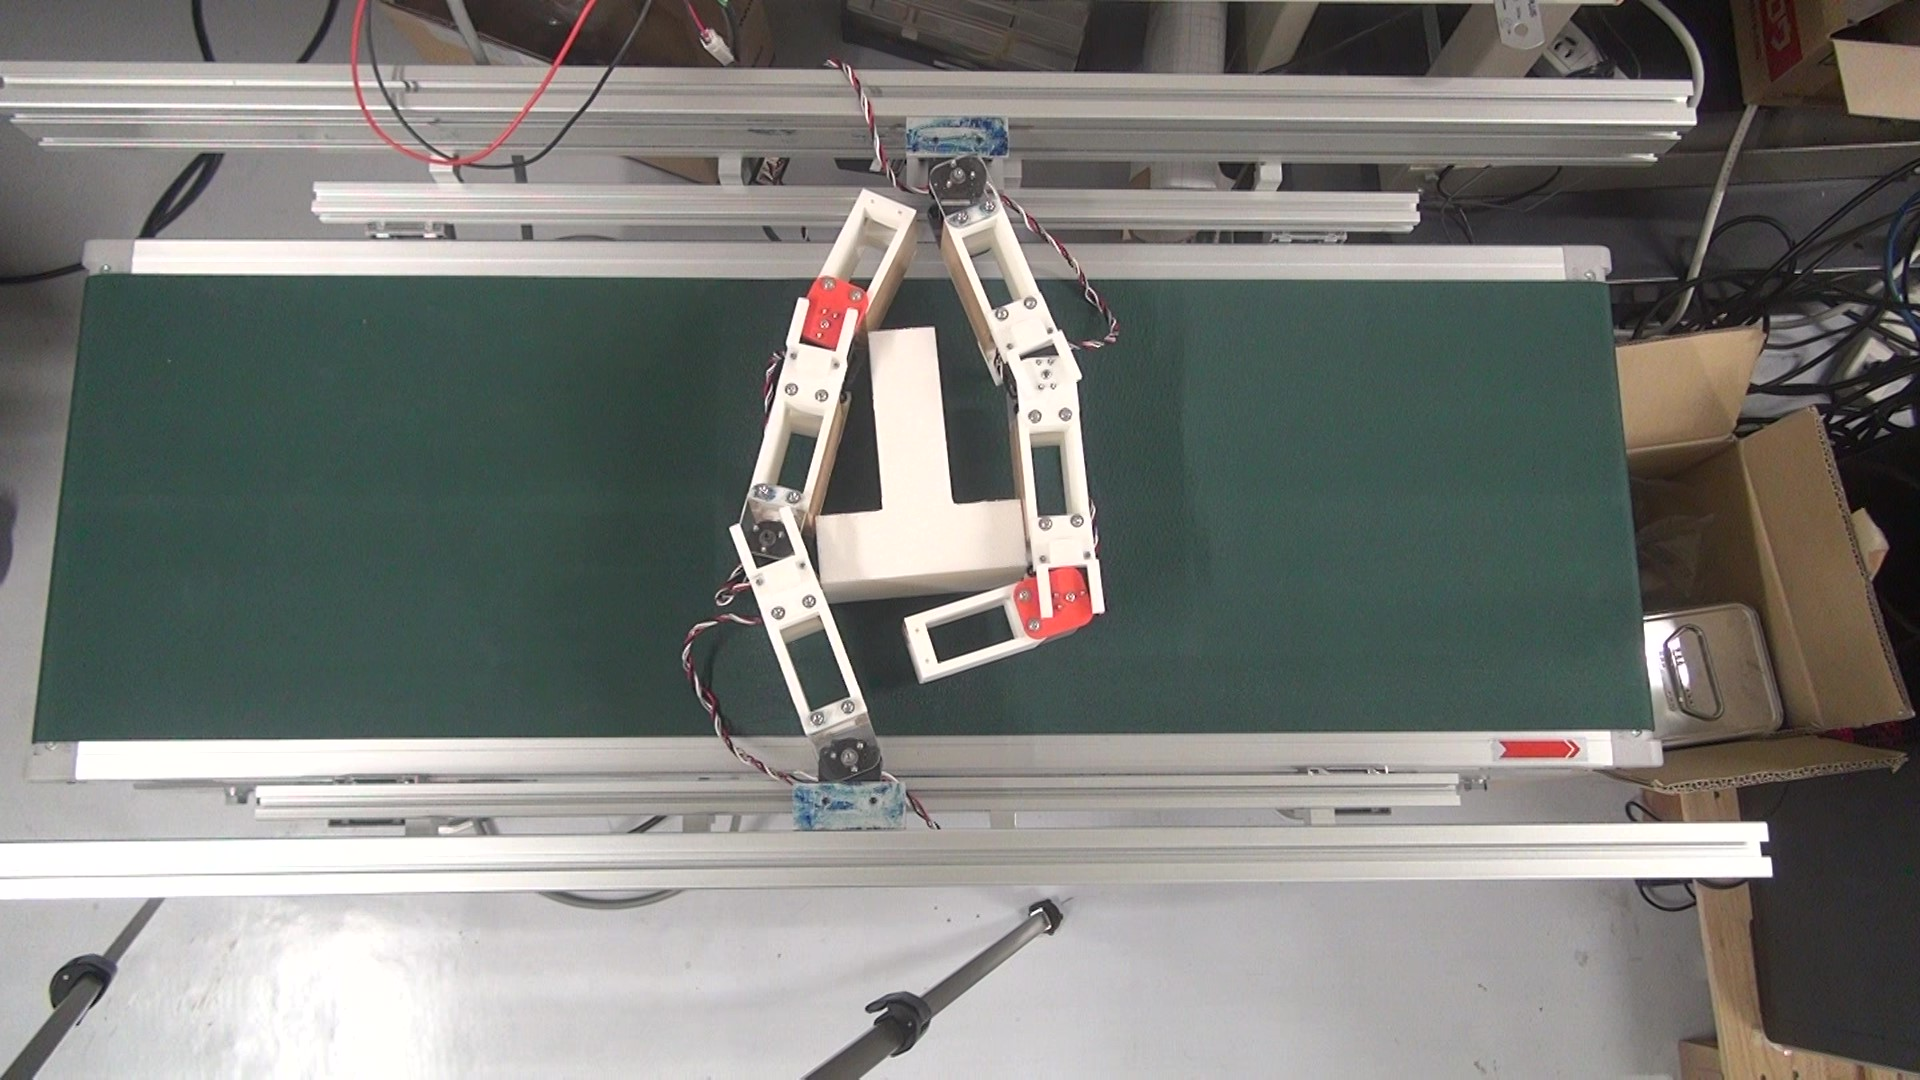
\includegraphics[width=0.98\hsize]{fig/4-manipulation-result/TShape/1-4.jpg}
\subcaption{}\label{}
\end{minipage}
\caption{TShape manipulation result \#1}\label{fig::result::tm1}
\end{figure}

\begin{figure}[hbt]
\centering
\begin{minipage}{0.249\hsize}
\centering
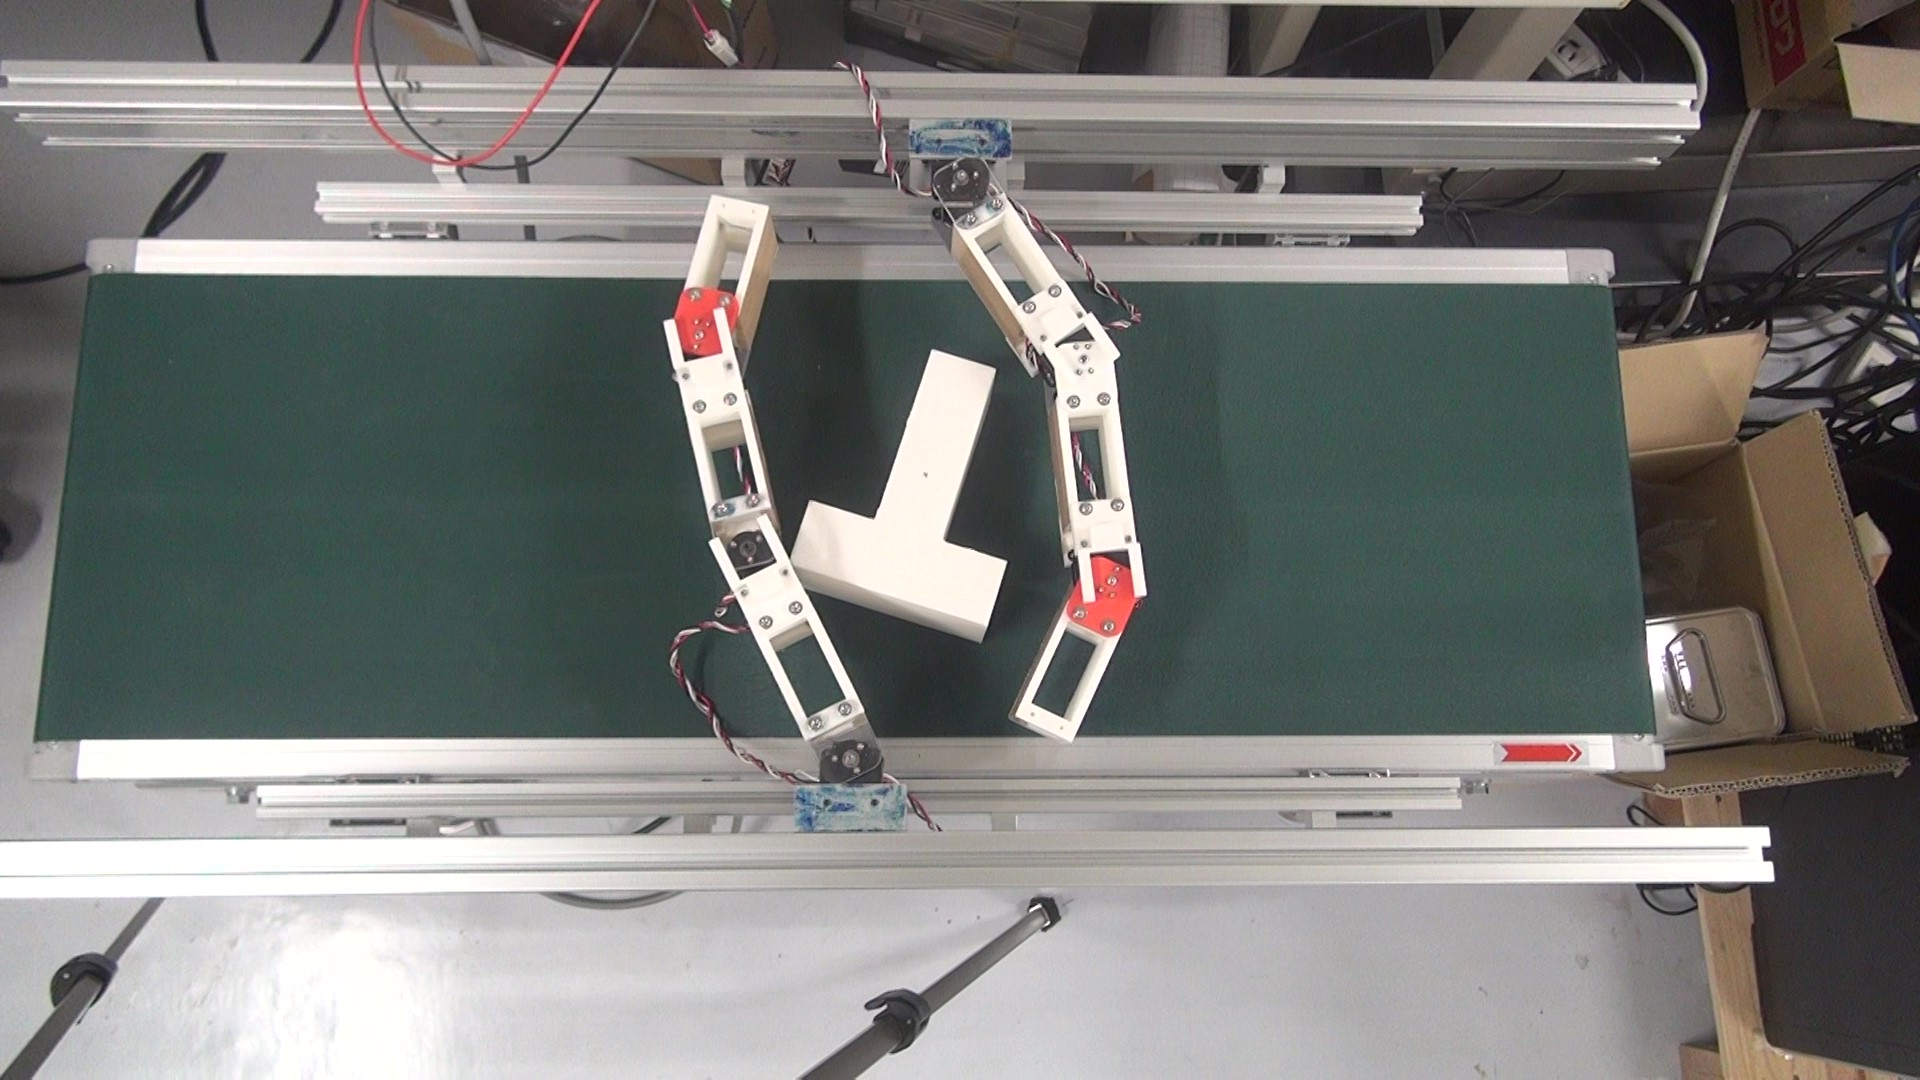
\includegraphics[width=0.98\hsize]{fig/4-manipulation-result/TShape/2-1.jpg}
\subcaption{}\label{}
\end{minipage}\hfill
\begin{minipage}{0.249\hsize}
\centering
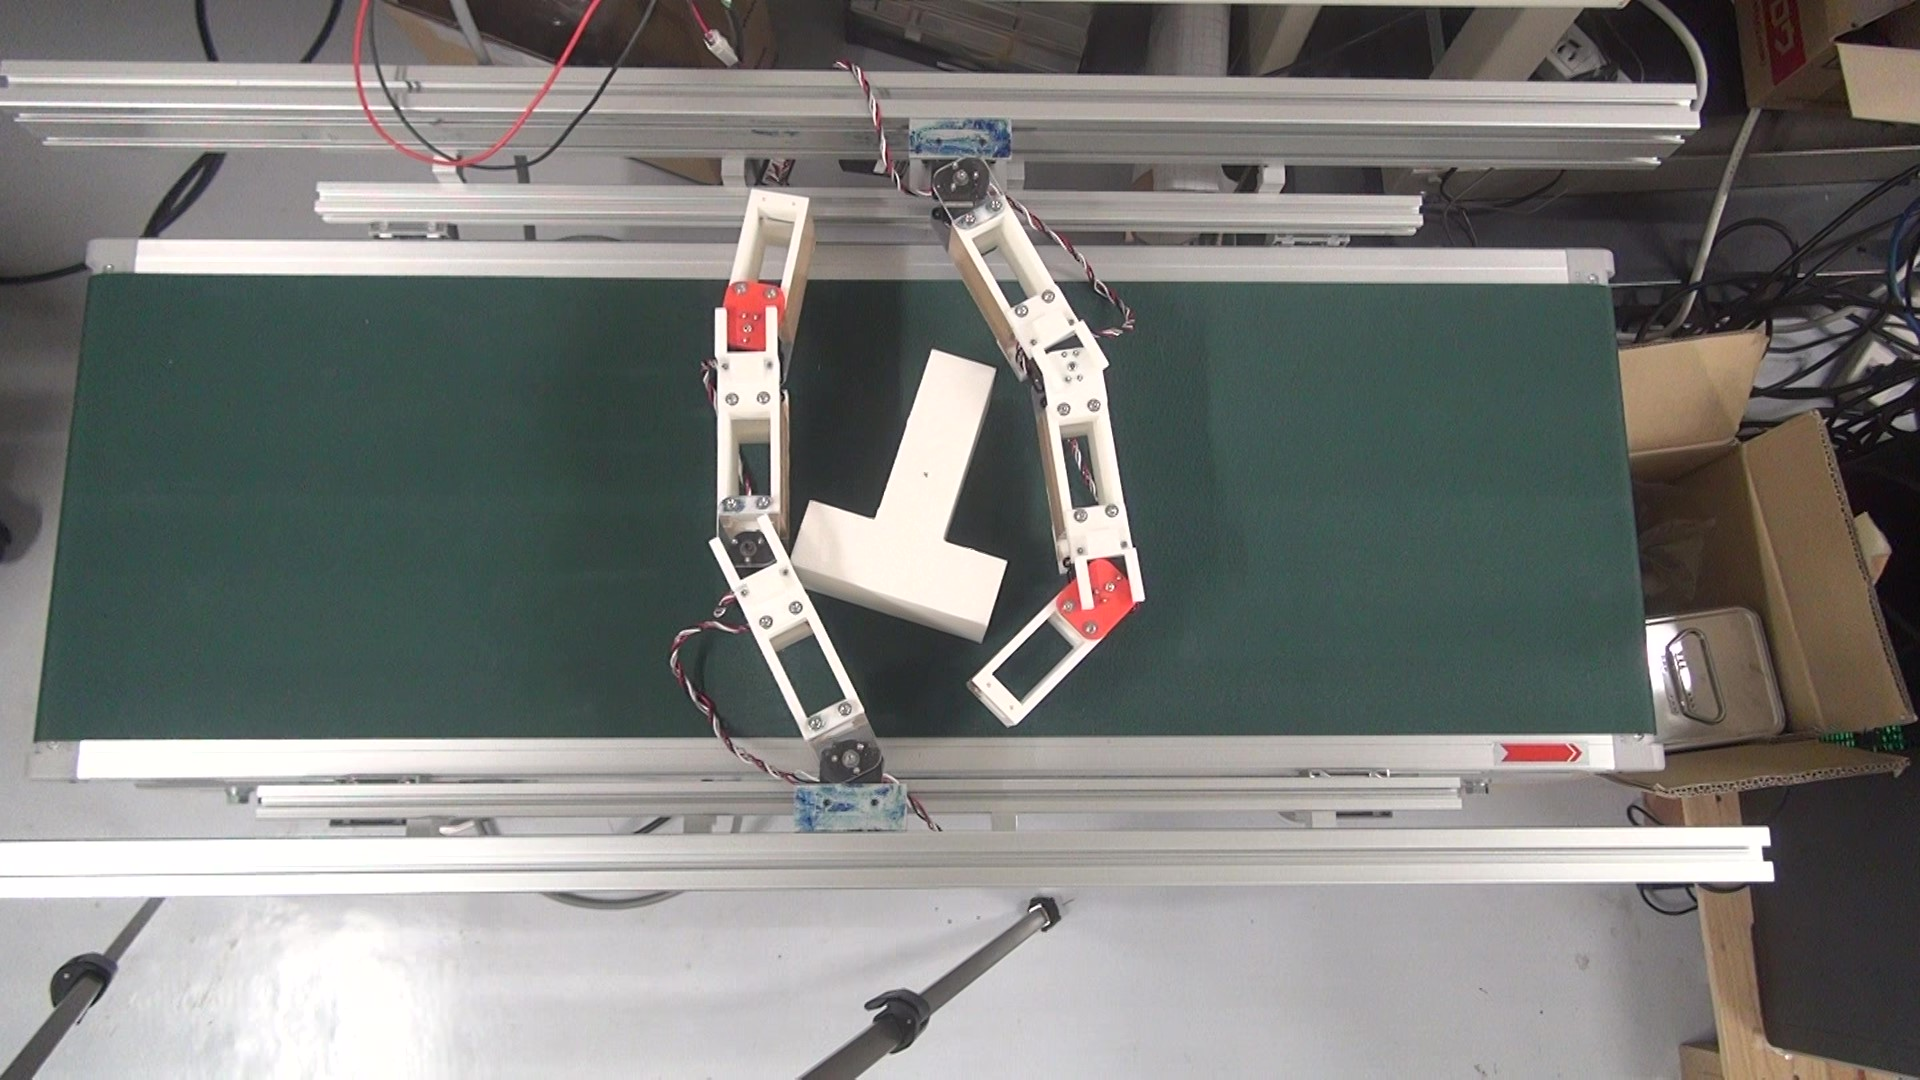
\includegraphics[width=0.98\hsize]{fig/4-manipulation-result/TShape/2-2.jpg}
\subcaption{}\label{}
\end{minipage}\hfill
\begin{minipage}{0.249\hsize}
\centering
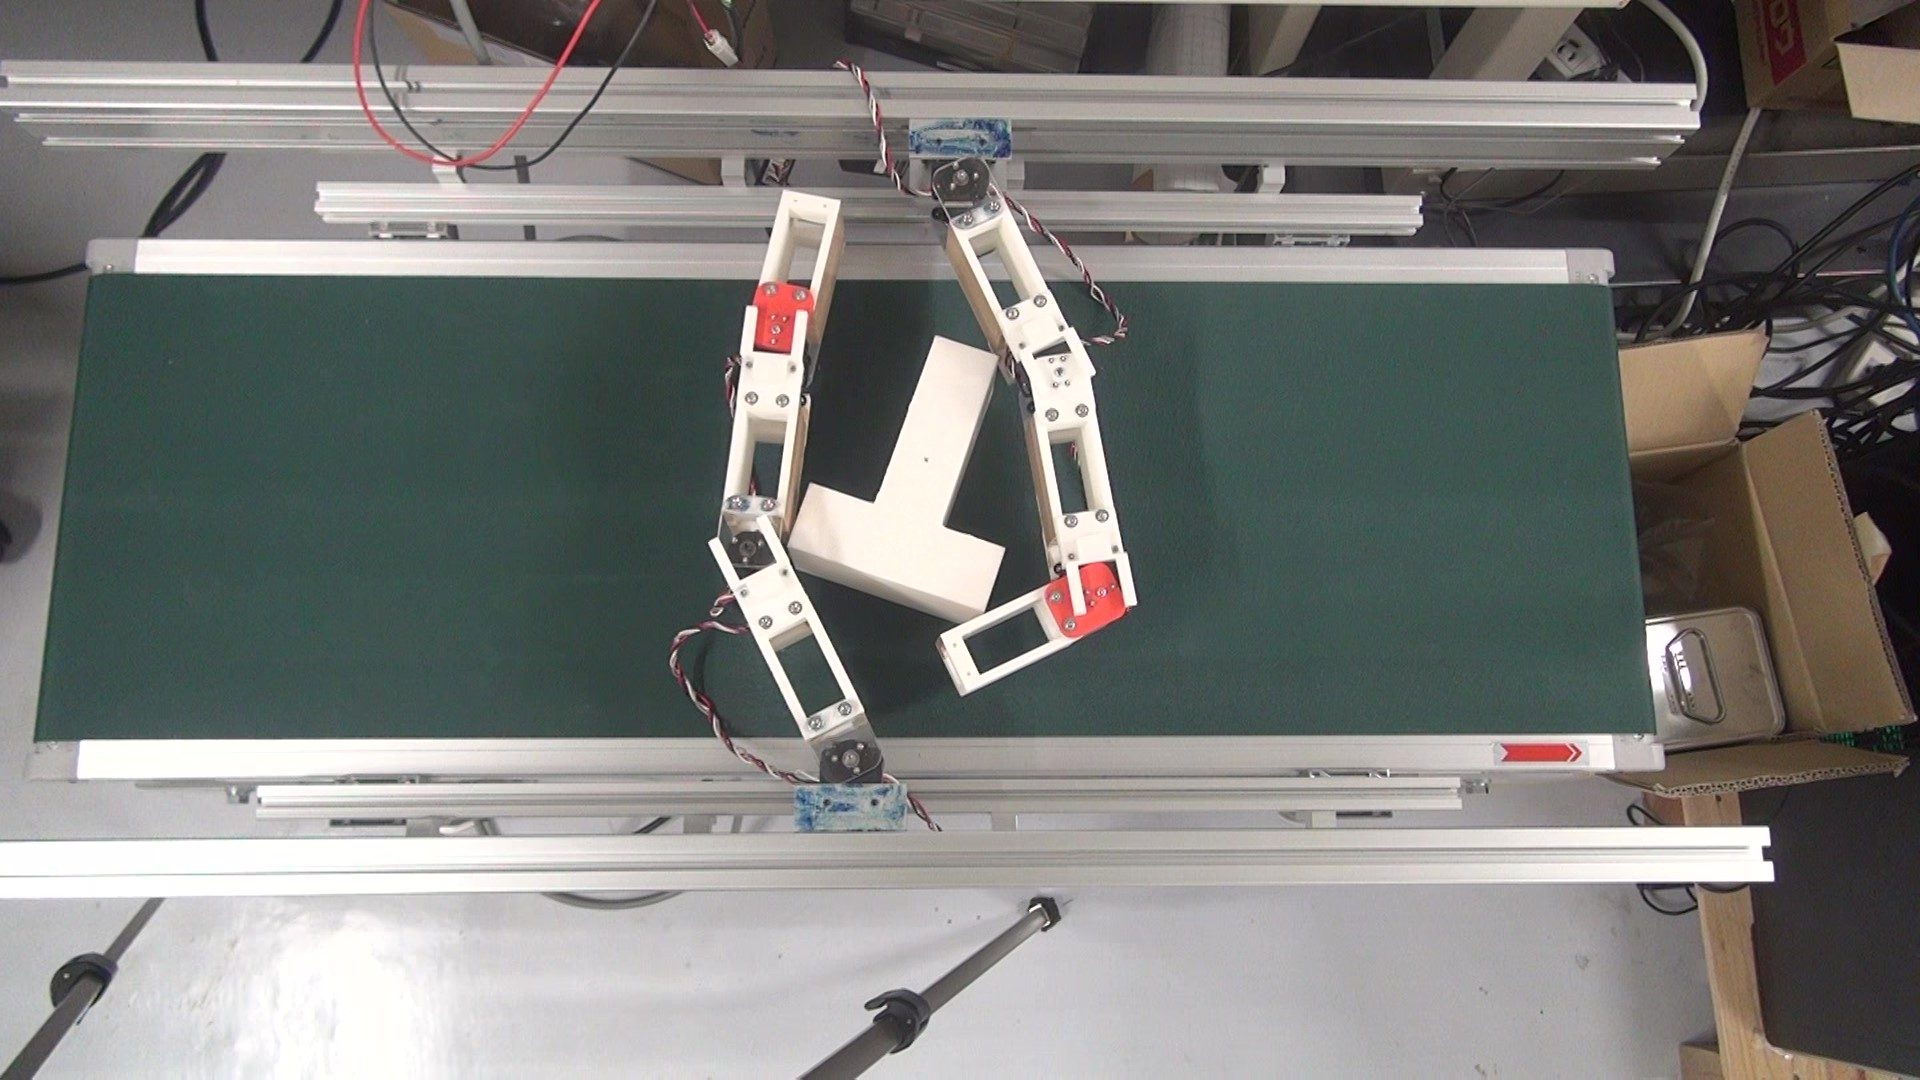
\includegraphics[width=0.98\hsize]{fig/4-manipulation-result/TShape/2-3.jpg}
\subcaption{}\label{}
\end{minipage}\hfill
\begin{minipage}{0.249\hsize}
\centering
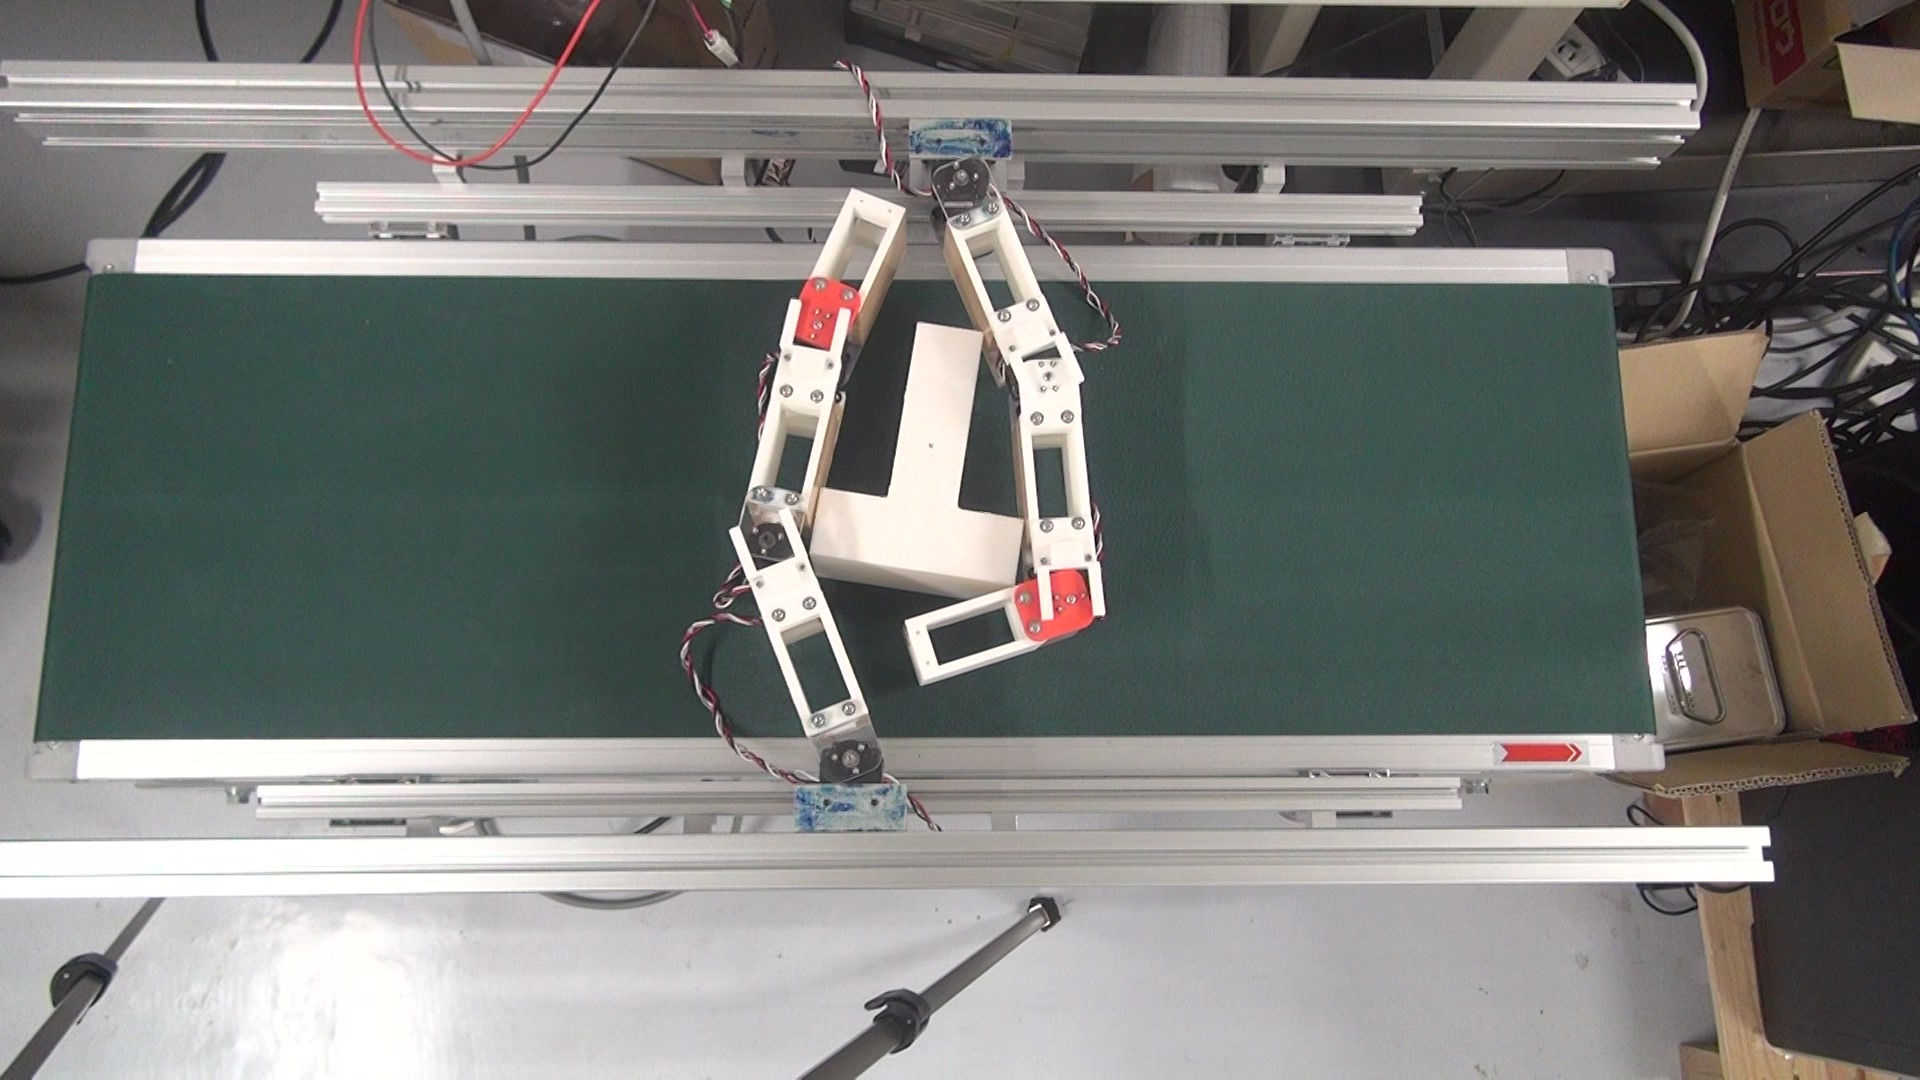
\includegraphics[width=0.98\hsize]{fig/4-manipulation-result/TShape/2-4.jpg}
\subcaption{}\label{}
\end{minipage}
\caption{TShape manipulation result \#2}\label{fig::result::tm2}
\end{figure}

\figref{fig::result::tm1}のマニピュレーション後の対象物位置・姿勢は,$(x, y, \phi) = (-5 \mathrm{[mm]}, 198 \mathrm{[mm]}, 3 \mathrm{[deg]})$であり,目標位置・姿勢から$\Delta y = -2 \mathrm{[mm]}$,$\Delta \phi = +3\mathrm{[deg]}$の誤差があった.また,\figref{fig::result::tm2}のマニピュレーション後の対象物位置・姿勢は,$(x, y, \phi) = (-10 \mathrm{[mm]}, 193 \mathrm{[mm]}, -6 \mathrm{[deg]})$であり,目標位置・姿勢から$\Delta y = -7 \mathrm{[mm]}$,$\Delta \phi = -6 \mathrm{[deg]}$の誤差があった.\par

次に,パーツフィーダとしての動作結果を\figref{fig::result::tp}に示す.これより,L字形物体に対してキャッチ,整列,リリースの一連のタスクを行えることを確認した.
\begin{figure}[hb]
\centering
\begin{minipage}{0.49\hsize}
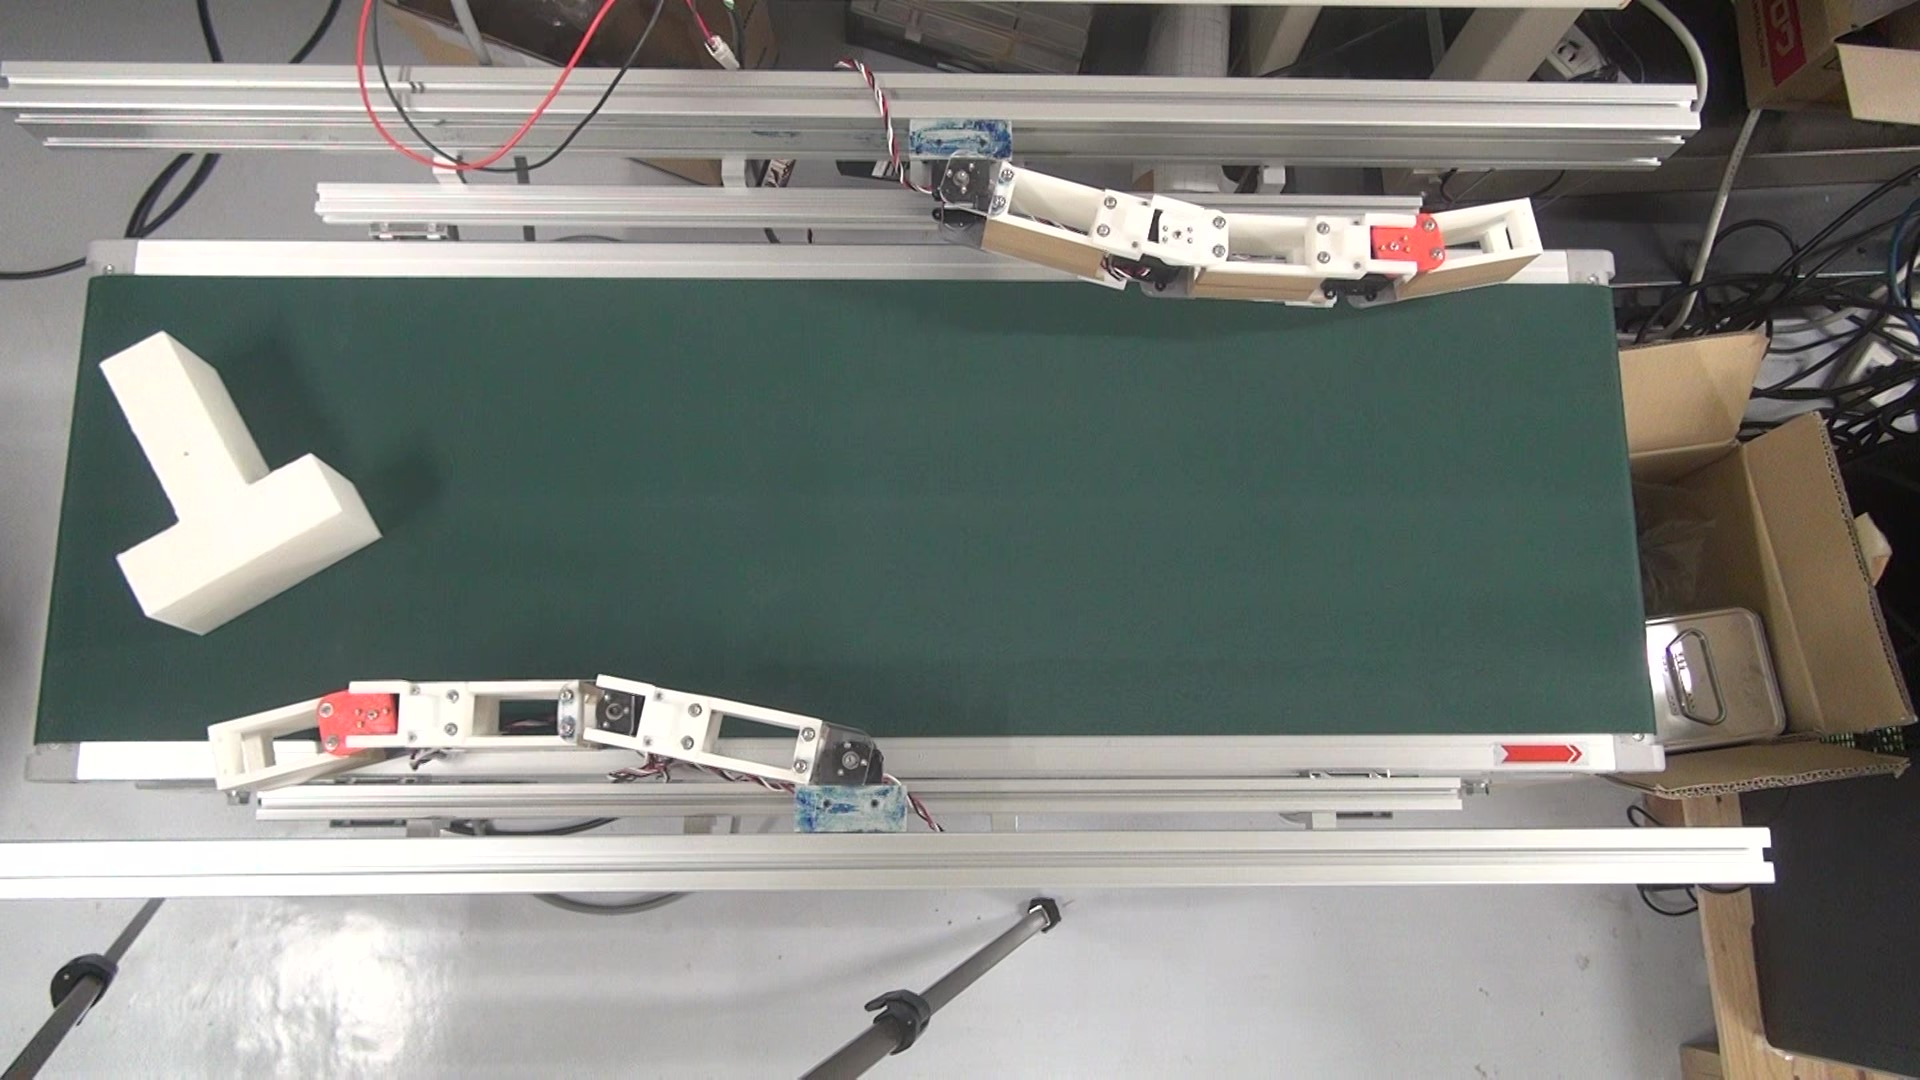
\includegraphics[width=0.98\hsize]{fig/4-manipulation-result/TShape/3-1.jpg}
\subcaption{}
\end{minipage}\hfill
\begin{minipage}{0.49\hsize}
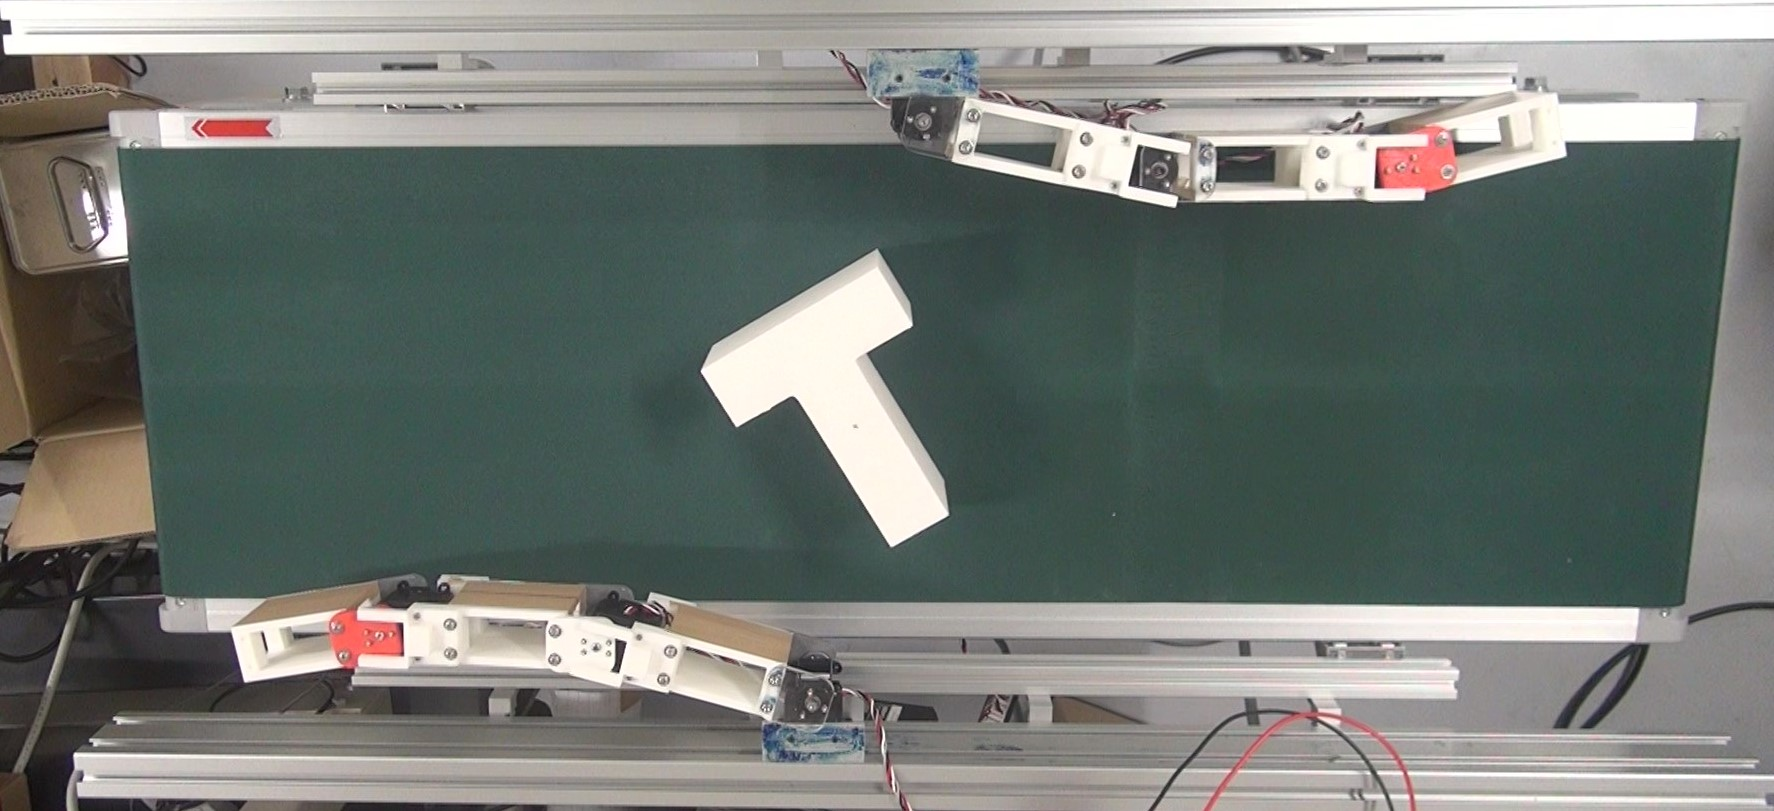
\includegraphics[width=0.98\hsize]{fig/4-manipulation-result/TShape/3-2.jpg}
\subcaption{}
\end{minipage}\hfill
\begin{minipage}{0.49\hsize}
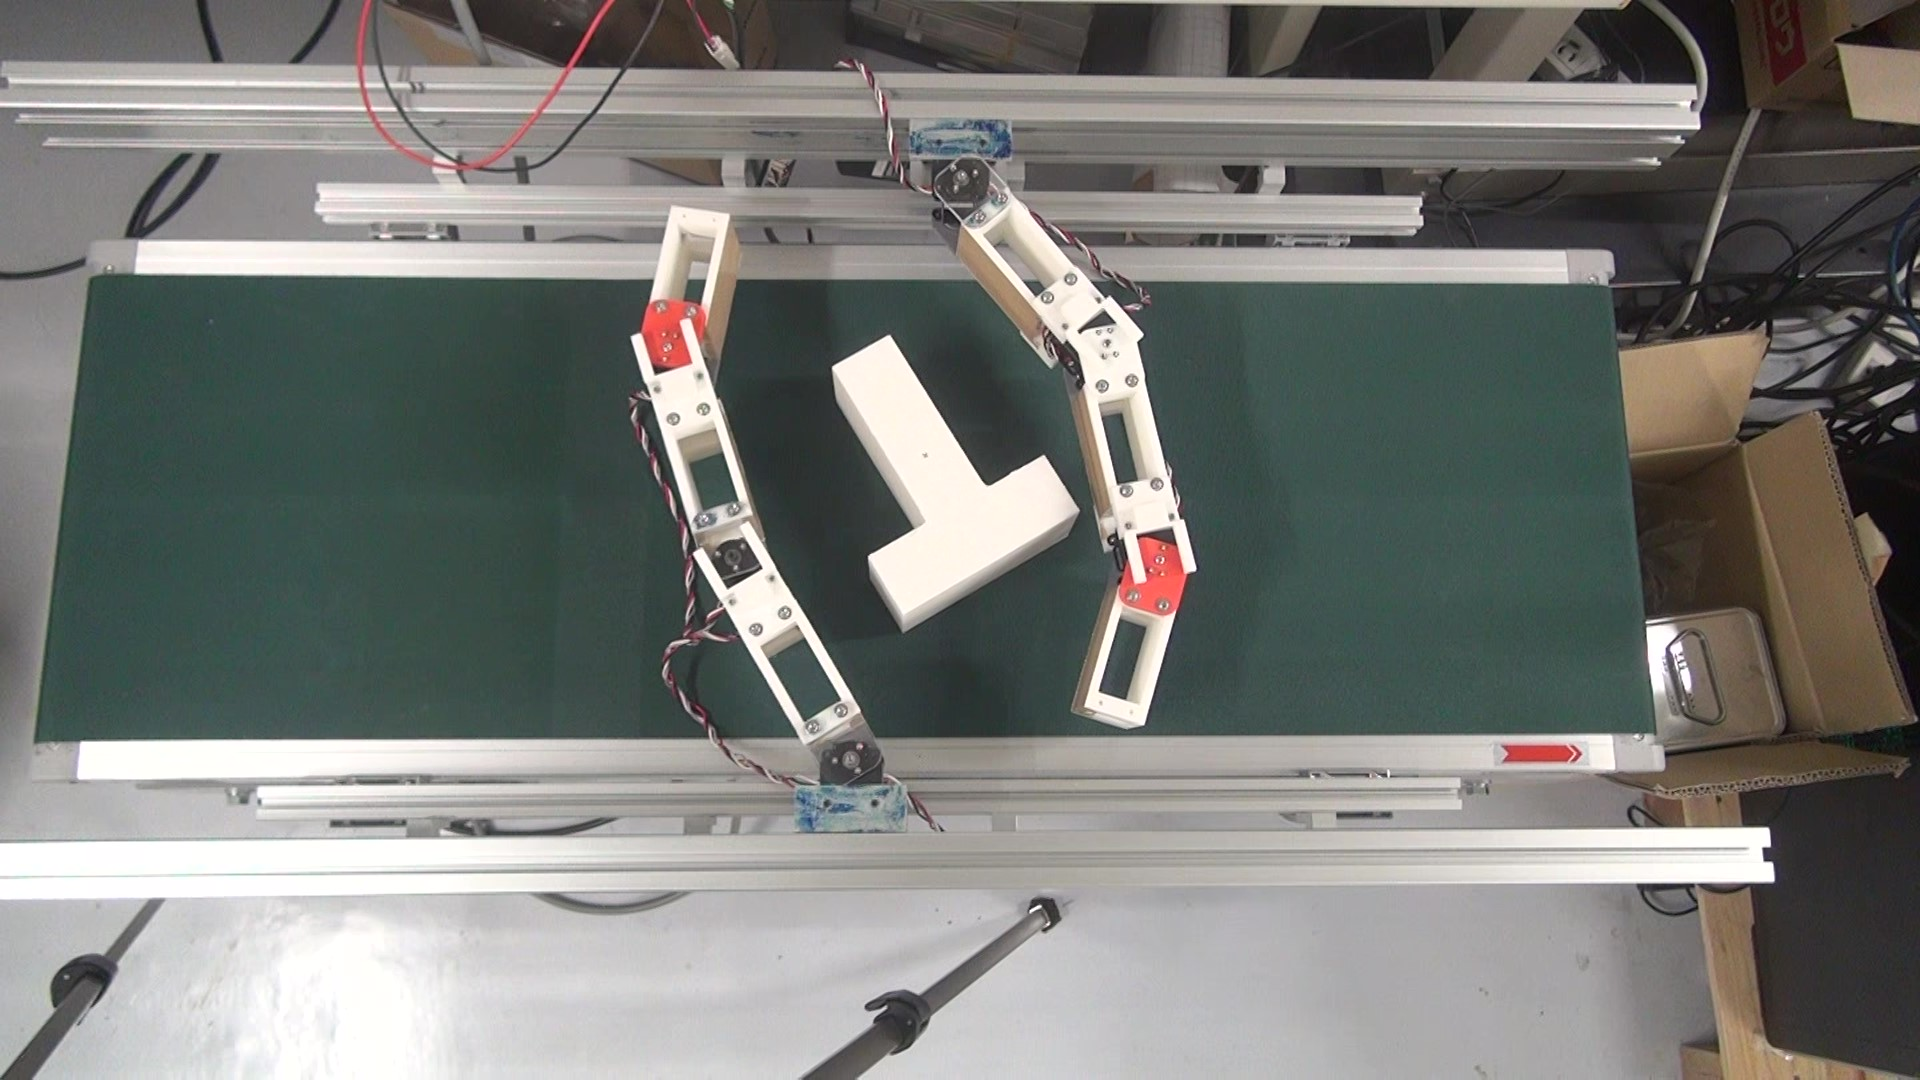
\includegraphics[width=0.98\hsize]{fig/4-manipulation-result/TShape/3-3.jpg}
\subcaption{}
\end{minipage}\hfill
\begin{minipage}{0.49\hsize}
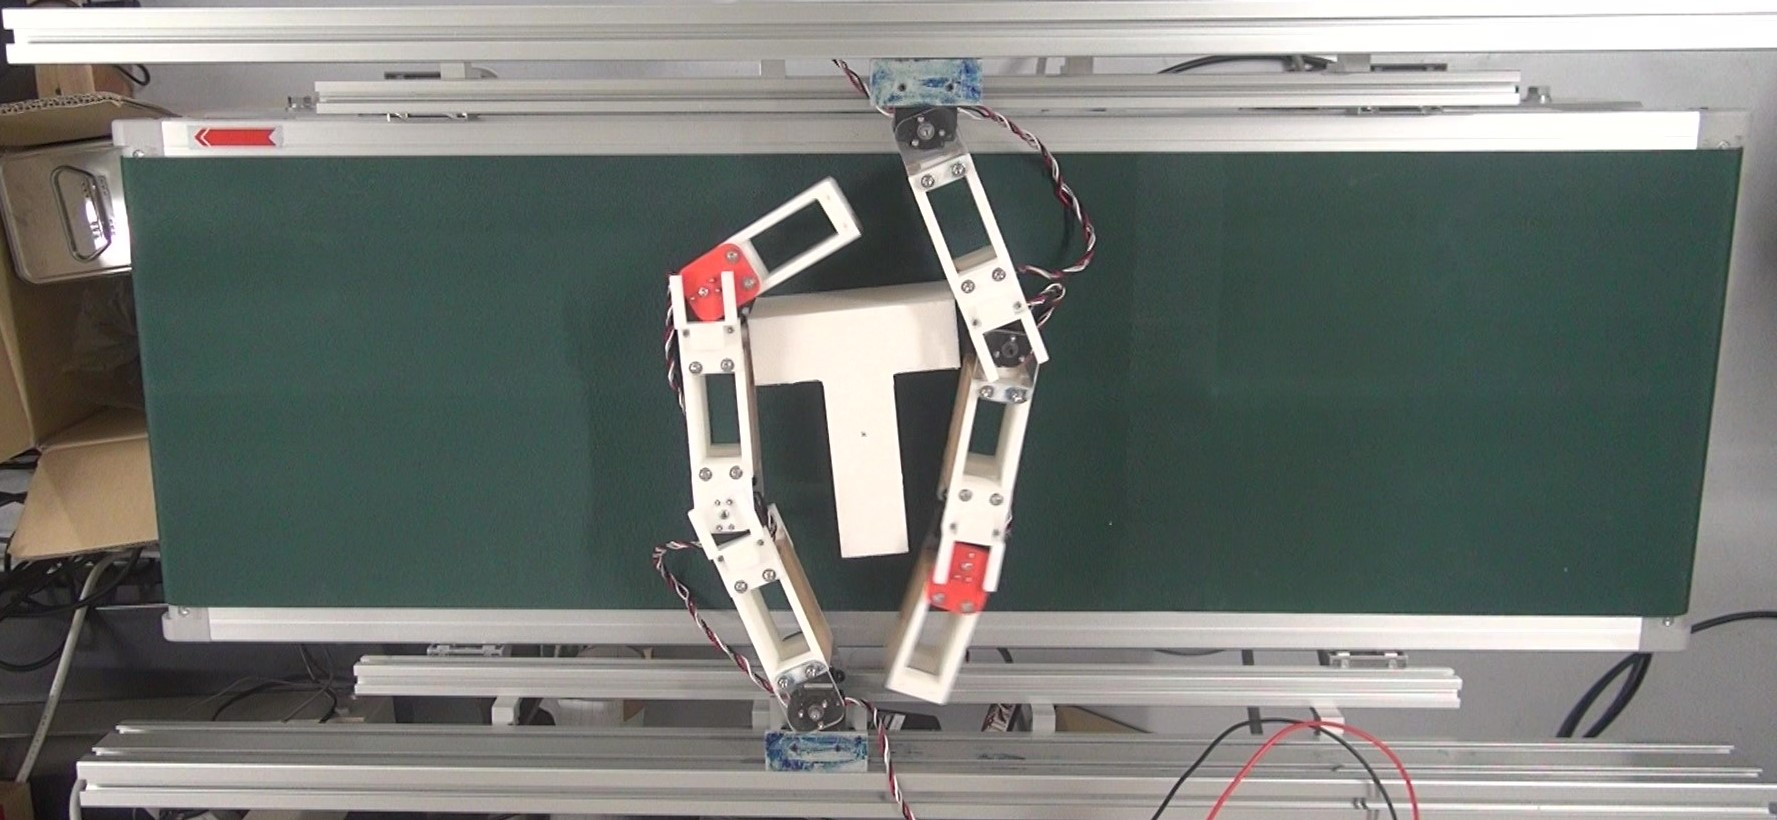
\includegraphics[width=0.98\hsize]{fig/4-manipulation-result/TShape/3-4.jpg}
\subcaption{}
\end{minipage}\hfill
\begin{minipage}{0.49\hsize}
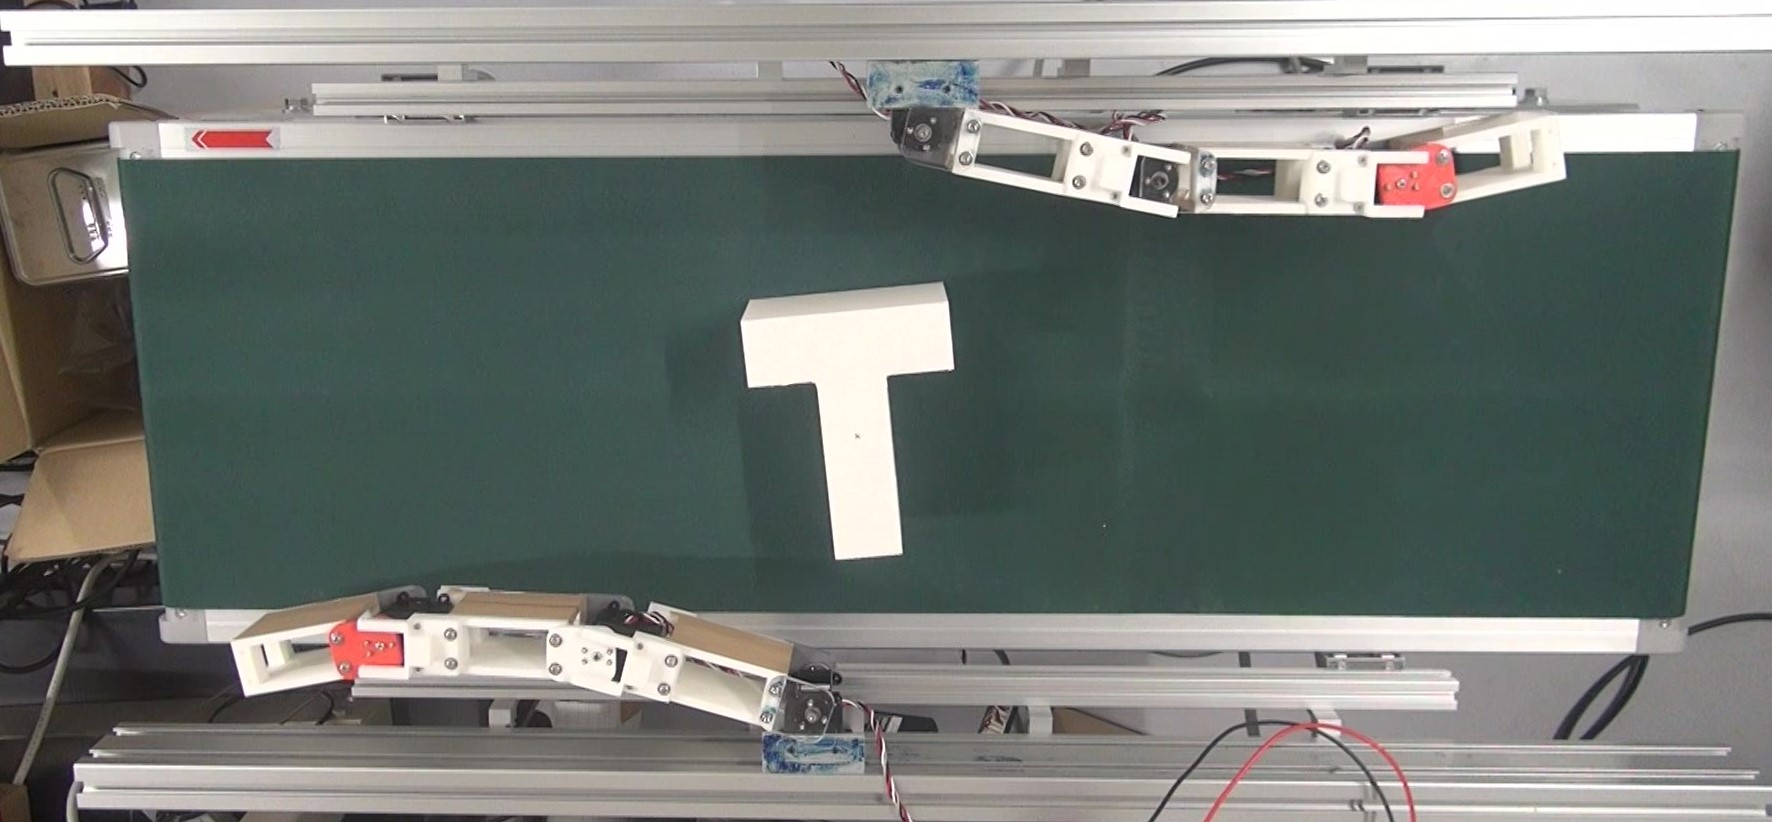
\includegraphics[width=0.98\hsize]{fig/4-manipulation-result/TShape/3-5.jpg}
\subcaption{}
\end{minipage}\hfill
\begin{minipage}{0.49\hsize}
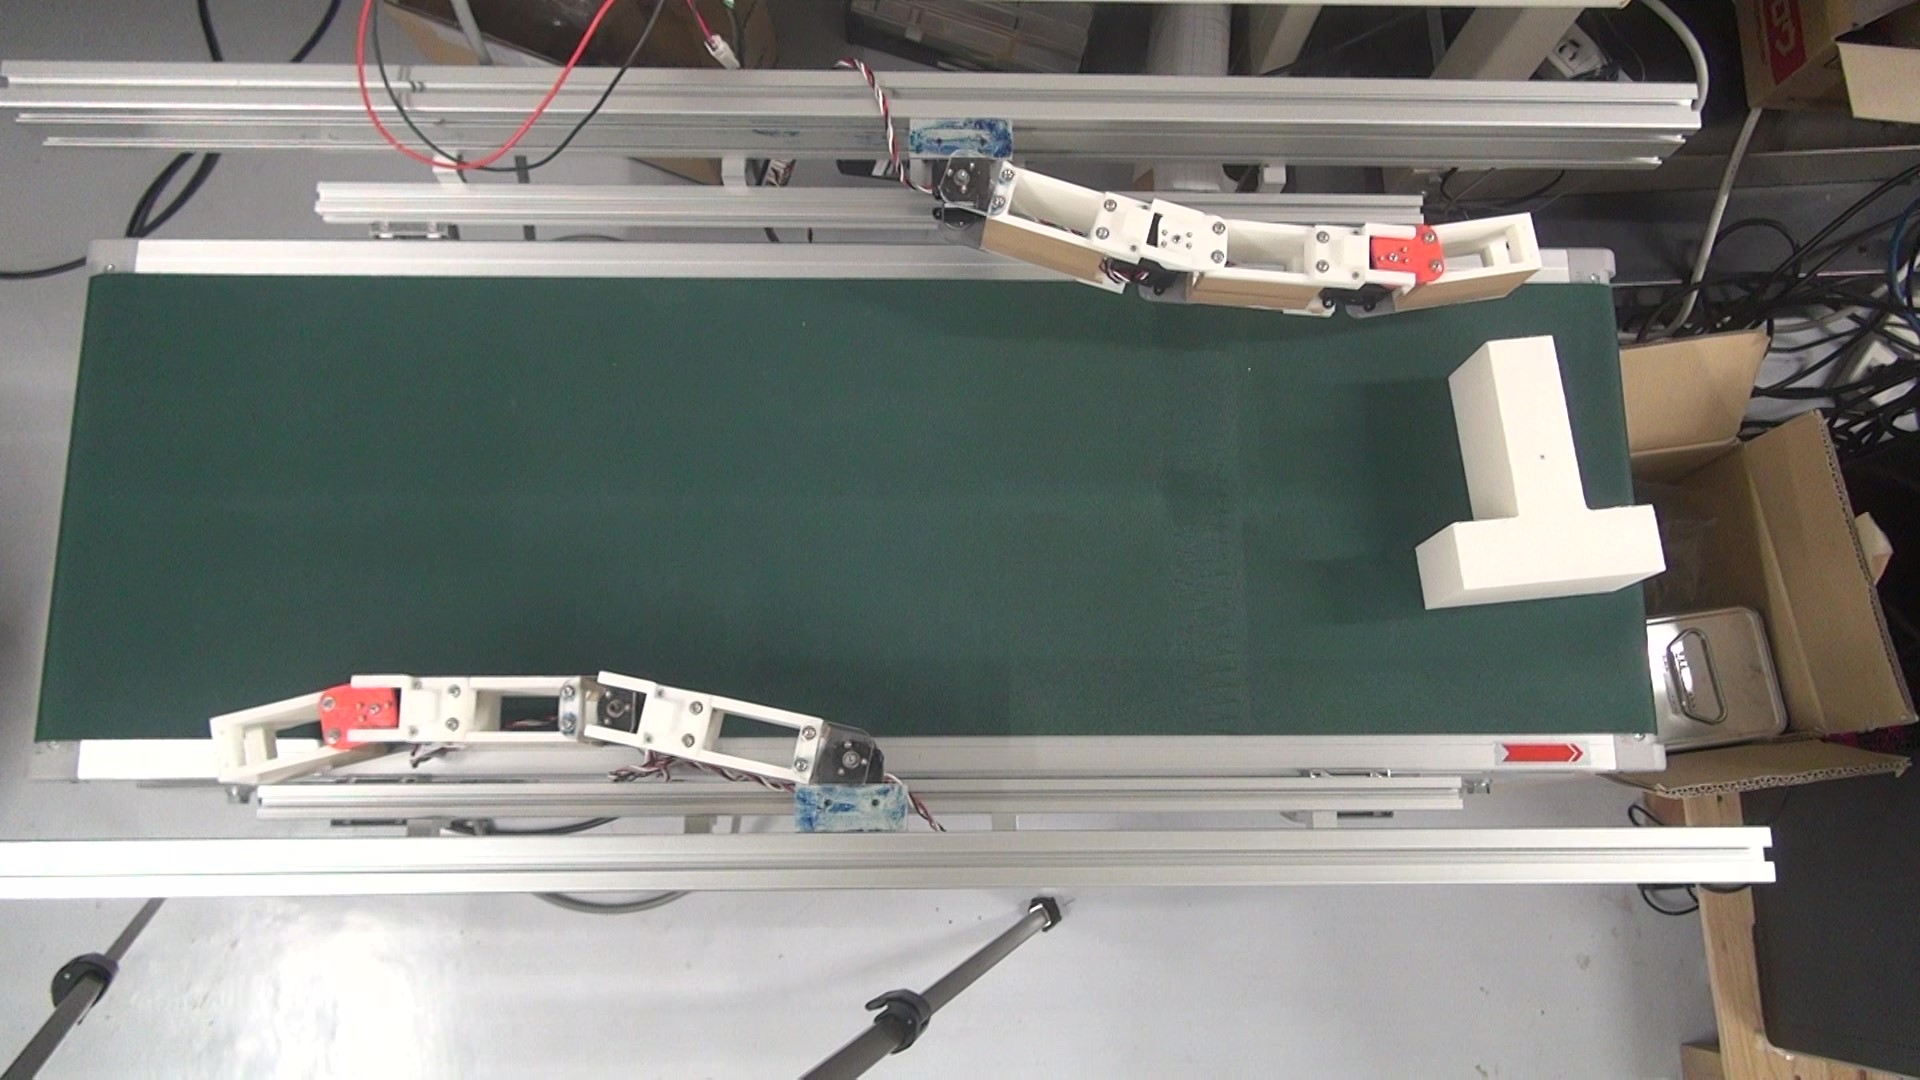
\includegraphics[width=0.98\hsize]{fig/4-manipulation-result/TShape/3-6.jpg}
\subcaption{}
\end{minipage}\hfill
\caption{TShape alignment as the parts feeder}\label{fig::result::tp}
\end{figure}



\section{考察} \label{sec::result::consideration}
順探索アルゴリズム,逆探索アルゴリズム,両側探索アルゴリズムのいずれのアルゴリズムで生成した経路でも,対象物をマニピュレーションできることを確認した.ここから,位置決め精度,ジャミングについて考察する.\par
位置決め精度には課題が残った.(例えば長方形物体では,動作計画でe=10だけれども実際はこれだけずれてた.)\par
原因は三つ考えられる.一つ目は,対象物のコンフィギュレーション離散空間の格子間距離である.前述の通り,現状は$(\Delta x, \Delta y, \Delta \phi) = (10 \mathrm{[mm]}, 10 \mathrm{[mm]}, 5 \mathrm{[deg]})$と設定している.そのため,実際には収束度$e$から$x$, $y$は$10 \mathrm{[mm]}$未満の,$\phi$は5 $\mathrm{[deg]}$未満のずれが生じうる.二つ目は,理論と実機の差異である.動作計画では,ハンドは指定された関節角度を取った状態で完全に固定されている.そのうえで対象物が取れる位置・姿勢を算出している.しかし実機では,対象物からの反力でハンドが指定姿勢から逸れうる.これによって,動作計画で想定されていない対象物位置・姿勢が取られ,最終的な位置決め精度にも影響を及ぼしている可能性がある.そのため,よりトルクの強いサーボモータを使うか,動作計画においてハンドのずれを補償するような処理を追加する必要がある.三つ目は,関節角が指定角度と異なることである.現在のハンドは3Dプリンタで生成したリンクにねじ穴をあけることで関節とリンクを固定しており,経年劣化で関節とリンクの間に遊びが生じてくる.また,\figref{}のようにハンドは片持ち状態となっているため,サーボモータにも負荷がかかり続け,指定角と実際の角度の間に誤差が生まれている可能性がある.後者の問題に関しては,各リンクにボールキャスタを取り付け,ベルトコンベア上を転がるようにすることで,片持ち状態を回避できサーボモータへの負荷も低減できると考えている.\par

次に,ジャミングに関して述べる.対向型ハンドの提案により,ジャミングの大部分は回避されたと考えている.実際,本章の検証実験ではジャミングの発生はなかった.しかし,稀にリンクとリンクの間隙に対象物の角が入り込み,ジャミングが発生する場合を確認している.これはハンドの設計に問題があり,例えば\figref{}のように角リンク間にリンク幅を直径とする円板を設置し,間隙を生じないようにすることで容易に解決できるジャミングであると考えている.従来の並列型ハンドで起きていたジャミングは,対象物とリンク間による摩擦によって発生していた場合が多く,こちらは回避が困難であった.対向型ハンドでは,このタイプのジャミングは確認されていないので,結論としてジャミングを解消できたと言える.




% 白魔術
\expandafter\ifx\csname ifdraft\endcsname\relax
    \end{document}
\fi
